% Generated by Sphinx.
\def\sphinxdocclass{report}
\documentclass[letterpaper,10pt,english]{sphinxmanual}
\usepackage[utf8]{inputenc}
\DeclareUnicodeCharacter{00A0}{\nobreakspace}
\usepackage{cmap}
\usepackage[T1]{fontenc}
\usepackage{babel}
\usepackage{times}
\usepackage[Bjarne]{fncychap}
\usepackage{longtable}
\usepackage{sphinx}
\usepackage{multirow}


\title{Zelig Documentation}
\date{August 25, 2014}
\release{5.0.1}
\author{The Zelig Team}
\newcommand{\sphinxlogo}{}
\renewcommand{\releasename}{Release}
\makeindex

\makeatletter
\def\PYG@reset{\let\PYG@it=\relax \let\PYG@bf=\relax%
    \let\PYG@ul=\relax \let\PYG@tc=\relax%
    \let\PYG@bc=\relax \let\PYG@ff=\relax}
\def\PYG@tok#1{\csname PYG@tok@#1\endcsname}
\def\PYG@toks#1+{\ifx\relax#1\empty\else%
    \PYG@tok{#1}\expandafter\PYG@toks\fi}
\def\PYG@do#1{\PYG@bc{\PYG@tc{\PYG@ul{%
    \PYG@it{\PYG@bf{\PYG@ff{#1}}}}}}}
\def\PYG#1#2{\PYG@reset\PYG@toks#1+\relax+\PYG@do{#2}}

\expandafter\def\csname PYG@tok@gd\endcsname{\def\PYG@tc##1{\textcolor[rgb]{0.63,0.00,0.00}{##1}}}
\expandafter\def\csname PYG@tok@gu\endcsname{\let\PYG@bf=\textbf\def\PYG@tc##1{\textcolor[rgb]{0.50,0.00,0.50}{##1}}}
\expandafter\def\csname PYG@tok@gt\endcsname{\def\PYG@tc##1{\textcolor[rgb]{0.00,0.27,0.87}{##1}}}
\expandafter\def\csname PYG@tok@gs\endcsname{\let\PYG@bf=\textbf}
\expandafter\def\csname PYG@tok@gr\endcsname{\def\PYG@tc##1{\textcolor[rgb]{1.00,0.00,0.00}{##1}}}
\expandafter\def\csname PYG@tok@cm\endcsname{\let\PYG@it=\textit\def\PYG@tc##1{\textcolor[rgb]{0.25,0.50,0.56}{##1}}}
\expandafter\def\csname PYG@tok@vg\endcsname{\def\PYG@tc##1{\textcolor[rgb]{0.73,0.38,0.84}{##1}}}
\expandafter\def\csname PYG@tok@m\endcsname{\def\PYG@tc##1{\textcolor[rgb]{0.13,0.50,0.31}{##1}}}
\expandafter\def\csname PYG@tok@mh\endcsname{\def\PYG@tc##1{\textcolor[rgb]{0.13,0.50,0.31}{##1}}}
\expandafter\def\csname PYG@tok@cs\endcsname{\def\PYG@tc##1{\textcolor[rgb]{0.25,0.50,0.56}{##1}}\def\PYG@bc##1{\setlength{\fboxsep}{0pt}\colorbox[rgb]{1.00,0.94,0.94}{\strut ##1}}}
\expandafter\def\csname PYG@tok@ge\endcsname{\let\PYG@it=\textit}
\expandafter\def\csname PYG@tok@vc\endcsname{\def\PYG@tc##1{\textcolor[rgb]{0.73,0.38,0.84}{##1}}}
\expandafter\def\csname PYG@tok@il\endcsname{\def\PYG@tc##1{\textcolor[rgb]{0.13,0.50,0.31}{##1}}}
\expandafter\def\csname PYG@tok@go\endcsname{\def\PYG@tc##1{\textcolor[rgb]{0.20,0.20,0.20}{##1}}}
\expandafter\def\csname PYG@tok@cp\endcsname{\def\PYG@tc##1{\textcolor[rgb]{0.00,0.44,0.13}{##1}}}
\expandafter\def\csname PYG@tok@gi\endcsname{\def\PYG@tc##1{\textcolor[rgb]{0.00,0.63,0.00}{##1}}}
\expandafter\def\csname PYG@tok@gh\endcsname{\let\PYG@bf=\textbf\def\PYG@tc##1{\textcolor[rgb]{0.00,0.00,0.50}{##1}}}
\expandafter\def\csname PYG@tok@ni\endcsname{\let\PYG@bf=\textbf\def\PYG@tc##1{\textcolor[rgb]{0.84,0.33,0.22}{##1}}}
\expandafter\def\csname PYG@tok@nl\endcsname{\let\PYG@bf=\textbf\def\PYG@tc##1{\textcolor[rgb]{0.00,0.13,0.44}{##1}}}
\expandafter\def\csname PYG@tok@nn\endcsname{\let\PYG@bf=\textbf\def\PYG@tc##1{\textcolor[rgb]{0.05,0.52,0.71}{##1}}}
\expandafter\def\csname PYG@tok@no\endcsname{\def\PYG@tc##1{\textcolor[rgb]{0.38,0.68,0.84}{##1}}}
\expandafter\def\csname PYG@tok@na\endcsname{\def\PYG@tc##1{\textcolor[rgb]{0.25,0.44,0.63}{##1}}}
\expandafter\def\csname PYG@tok@nb\endcsname{\def\PYG@tc##1{\textcolor[rgb]{0.00,0.44,0.13}{##1}}}
\expandafter\def\csname PYG@tok@nc\endcsname{\let\PYG@bf=\textbf\def\PYG@tc##1{\textcolor[rgb]{0.05,0.52,0.71}{##1}}}
\expandafter\def\csname PYG@tok@nd\endcsname{\let\PYG@bf=\textbf\def\PYG@tc##1{\textcolor[rgb]{0.33,0.33,0.33}{##1}}}
\expandafter\def\csname PYG@tok@ne\endcsname{\def\PYG@tc##1{\textcolor[rgb]{0.00,0.44,0.13}{##1}}}
\expandafter\def\csname PYG@tok@nf\endcsname{\def\PYG@tc##1{\textcolor[rgb]{0.02,0.16,0.49}{##1}}}
\expandafter\def\csname PYG@tok@si\endcsname{\let\PYG@it=\textit\def\PYG@tc##1{\textcolor[rgb]{0.44,0.63,0.82}{##1}}}
\expandafter\def\csname PYG@tok@s2\endcsname{\def\PYG@tc##1{\textcolor[rgb]{0.25,0.44,0.63}{##1}}}
\expandafter\def\csname PYG@tok@vi\endcsname{\def\PYG@tc##1{\textcolor[rgb]{0.73,0.38,0.84}{##1}}}
\expandafter\def\csname PYG@tok@nt\endcsname{\let\PYG@bf=\textbf\def\PYG@tc##1{\textcolor[rgb]{0.02,0.16,0.45}{##1}}}
\expandafter\def\csname PYG@tok@nv\endcsname{\def\PYG@tc##1{\textcolor[rgb]{0.73,0.38,0.84}{##1}}}
\expandafter\def\csname PYG@tok@s1\endcsname{\def\PYG@tc##1{\textcolor[rgb]{0.25,0.44,0.63}{##1}}}
\expandafter\def\csname PYG@tok@gp\endcsname{\let\PYG@bf=\textbf\def\PYG@tc##1{\textcolor[rgb]{0.78,0.36,0.04}{##1}}}
\expandafter\def\csname PYG@tok@sh\endcsname{\def\PYG@tc##1{\textcolor[rgb]{0.25,0.44,0.63}{##1}}}
\expandafter\def\csname PYG@tok@ow\endcsname{\let\PYG@bf=\textbf\def\PYG@tc##1{\textcolor[rgb]{0.00,0.44,0.13}{##1}}}
\expandafter\def\csname PYG@tok@sx\endcsname{\def\PYG@tc##1{\textcolor[rgb]{0.78,0.36,0.04}{##1}}}
\expandafter\def\csname PYG@tok@bp\endcsname{\def\PYG@tc##1{\textcolor[rgb]{0.00,0.44,0.13}{##1}}}
\expandafter\def\csname PYG@tok@c1\endcsname{\let\PYG@it=\textit\def\PYG@tc##1{\textcolor[rgb]{0.25,0.50,0.56}{##1}}}
\expandafter\def\csname PYG@tok@kc\endcsname{\let\PYG@bf=\textbf\def\PYG@tc##1{\textcolor[rgb]{0.00,0.44,0.13}{##1}}}
\expandafter\def\csname PYG@tok@c\endcsname{\let\PYG@it=\textit\def\PYG@tc##1{\textcolor[rgb]{0.25,0.50,0.56}{##1}}}
\expandafter\def\csname PYG@tok@mf\endcsname{\def\PYG@tc##1{\textcolor[rgb]{0.13,0.50,0.31}{##1}}}
\expandafter\def\csname PYG@tok@err\endcsname{\def\PYG@bc##1{\setlength{\fboxsep}{0pt}\fcolorbox[rgb]{1.00,0.00,0.00}{1,1,1}{\strut ##1}}}
\expandafter\def\csname PYG@tok@kd\endcsname{\let\PYG@bf=\textbf\def\PYG@tc##1{\textcolor[rgb]{0.00,0.44,0.13}{##1}}}
\expandafter\def\csname PYG@tok@ss\endcsname{\def\PYG@tc##1{\textcolor[rgb]{0.32,0.47,0.09}{##1}}}
\expandafter\def\csname PYG@tok@sr\endcsname{\def\PYG@tc##1{\textcolor[rgb]{0.14,0.33,0.53}{##1}}}
\expandafter\def\csname PYG@tok@mo\endcsname{\def\PYG@tc##1{\textcolor[rgb]{0.13,0.50,0.31}{##1}}}
\expandafter\def\csname PYG@tok@mi\endcsname{\def\PYG@tc##1{\textcolor[rgb]{0.13,0.50,0.31}{##1}}}
\expandafter\def\csname PYG@tok@kn\endcsname{\let\PYG@bf=\textbf\def\PYG@tc##1{\textcolor[rgb]{0.00,0.44,0.13}{##1}}}
\expandafter\def\csname PYG@tok@o\endcsname{\def\PYG@tc##1{\textcolor[rgb]{0.40,0.40,0.40}{##1}}}
\expandafter\def\csname PYG@tok@kr\endcsname{\let\PYG@bf=\textbf\def\PYG@tc##1{\textcolor[rgb]{0.00,0.44,0.13}{##1}}}
\expandafter\def\csname PYG@tok@s\endcsname{\def\PYG@tc##1{\textcolor[rgb]{0.25,0.44,0.63}{##1}}}
\expandafter\def\csname PYG@tok@kp\endcsname{\def\PYG@tc##1{\textcolor[rgb]{0.00,0.44,0.13}{##1}}}
\expandafter\def\csname PYG@tok@w\endcsname{\def\PYG@tc##1{\textcolor[rgb]{0.73,0.73,0.73}{##1}}}
\expandafter\def\csname PYG@tok@kt\endcsname{\def\PYG@tc##1{\textcolor[rgb]{0.56,0.13,0.00}{##1}}}
\expandafter\def\csname PYG@tok@sc\endcsname{\def\PYG@tc##1{\textcolor[rgb]{0.25,0.44,0.63}{##1}}}
\expandafter\def\csname PYG@tok@sb\endcsname{\def\PYG@tc##1{\textcolor[rgb]{0.25,0.44,0.63}{##1}}}
\expandafter\def\csname PYG@tok@k\endcsname{\let\PYG@bf=\textbf\def\PYG@tc##1{\textcolor[rgb]{0.00,0.44,0.13}{##1}}}
\expandafter\def\csname PYG@tok@se\endcsname{\let\PYG@bf=\textbf\def\PYG@tc##1{\textcolor[rgb]{0.25,0.44,0.63}{##1}}}
\expandafter\def\csname PYG@tok@sd\endcsname{\let\PYG@it=\textit\def\PYG@tc##1{\textcolor[rgb]{0.25,0.44,0.63}{##1}}}

\def\PYGZbs{\char`\\}
\def\PYGZus{\char`\_}
\def\PYGZob{\char`\{}
\def\PYGZcb{\char`\}}
\def\PYGZca{\char`\^}
\def\PYGZam{\char`\&}
\def\PYGZlt{\char`\<}
\def\PYGZgt{\char`\>}
\def\PYGZsh{\char`\#}
\def\PYGZpc{\char`\%}
\def\PYGZdl{\char`\$}
\def\PYGZhy{\char`\-}
\def\PYGZsq{\char`\'}
\def\PYGZdq{\char`\"}
\def\PYGZti{\char`\~}
% for compatibility with earlier versions
\def\PYGZat{@}
\def\PYGZlb{[}
\def\PYGZrb{]}
\makeatother

\begin{document}

\maketitle
\tableofcontents
\phantomsection\label{index::doc}


\textbf{Zelig} is a framework for interfacing with a wide range of statistical models and analytic methods in a common and simple way. Above and beyond estimation, it adds considerable infrastructure to existing heterogeneous R implementations by translating coefficient estimates into interpretable quantities of interest and automating statistical procedures (e.g., bootstrapping) though an intelligible call structure.

To get started, we recommend following the {\hyperref[installation_quickstart:installation-quickstart]{\emph{Installation and Quickstart}}} guide. More information about the software, including our technical vision and goals for the project, can be found at the {\hyperref[about:about]{\emph{About Zelig}}} page.

To view the code-base, visit the source repository at \href{https://github.com/IQSS/Zelig}{https://github.com/IQSS/Zelig} and for regular updates  and release information be sure to follow us on twitter at \href{https://twitter.com/IQSS}{@IQSS}. We also recommend joining the \href{https://groups.google.com/forum/\#!forum/zelig-statistical-software}{Zelig Google Group}, where we are encouraging users to ask questions, report bugs, and help others.

We can also get the \href{http://zeligproject.org/build/latex/Zelig.pdf}{PDF}
of the documentation.


\chapter{Installation and Quickstart}
\label{installation_quickstart::doc}\label{installation_quickstart:welcome-to-zelig}\label{installation_quickstart:installation-and-quickstart}\label{installation_quickstart:installation-quickstart}
This guide is designed to get you up and running with the current \emph{beta} release of Zelig (5.0.1).


\bigskip\hrule{}\bigskip



\section{Installing R and Zelig}
\label{installation_quickstart:installing-r-and-zelig}
Before using Zelig, you will need to download and install both the R statistical program and the Zelig package:

\textbf{Installing R}

To install R, go to \href{http://www.r-project.org/}{http://www.r-project.org/}  Select the \code{CRAN} option from the left-hand menu (CRAN is the Comprehensive R Archive Network where all files related to R can be found). Pick a CRAN mirror closest to your current geographic location (there are multiple mirrors of this database in various locations, selecting the one closest to you will be sure to maximize your the speed of your download).  Follow the instructions for downloading R for Linux, Mac OS X, or Windows.


\bigskip\hrule{}\bigskip


\textbf{Installing Zelig}

Because Zelig 5 is still a \emph{beta} release and is not yet available on \code{CRAN} (with other R software packages), it must be downloaded from Github using the \code{devtools} package.

Once you've successfully installed R, open it, and at the terminal prompt, type in the following commands verbatim:

\begin{Verbatim}[commandchars=\\\{\}]
\PYG{c+c1}{\PYGZsh{} This installs devtools package, if not already installed}
install.packages\PYG{p}{(}\PYG{l+s}{\PYGZdq{}}\PYG{l+s}{devtools\PYGZdq{}}\PYG{p}{)}
\PYG{c+c1}{\PYGZsh{} This loads devtools}
library\PYG{p}{(}devtools\PYG{p}{)}
\PYG{c+c1}{\PYGZsh{} This downloads Zelig 5.0.1 from the IQSS Github repo}
install\PYGZus{}github\PYG{p}{(}\PYG{l+s}{\PYGZsq{}}\PYG{l+s}{IQSS/Zelig\PYGZsq{}}\PYG{p}{)}
\end{Verbatim}

If you have successfully installed the program, you will see a the following message: \emph{``DONE (Zelig5)''}.


\bigskip\hrule{}\bigskip



\section{Quickstart Guide}
\label{installation_quickstart:quickstart-guide}
Now that we have successfully downloaded and installed Zelig from Github, we will load the package and walk through am example. The scenario is a simple one: imagine you want to estimate the distance a car has traveled given it's speed and you have a dataset of cars, distance and speed. Throughout the rest of this guide, we will walk you through building a statistical model from this data using Zelig.

\textbf{Loading Zelig}

First, we have to load Zelig into R. After installing both R and
Zelig, open R and type:

\begin{Verbatim}[commandchars=\\\{\}]
library\PYG{p}{(}Zelig5\PYG{p}{)}
\end{Verbatim}


\bigskip\hrule{}\bigskip


\textbf{Building Models}

Now, lets build a statistical model that captures the relationship a cars distance and speed, where distance is the outcome (dependent) variable and speed is the only explanatory (independent) variable. Given that distance (the DV) is a continuous variable, we should use a least squares regression.

To do so, we must first create Zelig least squares object, then specify our model, and finally regress distance on speed to estimate the relationship between speed and distance:

\begin{Verbatim}[commandchars=\\\{\}]
\PYG{c+c1}{\PYGZsh{} load toy dataset (when you install R, example datasets are also installed)}
data\PYG{p}{(}cars\PYG{p}{)}
\PYG{c+c1}{\PYGZsh{} initialize Zelig5 least squares object}
z5 \PYG{o}{\PYGZlt{}\PYGZhy{}} zls\PYG{o}{\PYGZdl{}}new\PYG{p}{(}\PYG{p}{)}
\PYG{c+c1}{\PYGZsh{} estimate ls model}
z5\PYG{o}{\PYGZdl{}}zelig\PYG{p}{(}dist \PYG{o}{\PYGZti{}} speed\PYG{p}{,} data \PYG{o}{=} cars\PYG{p}{)}
\PYG{c+c1}{\PYGZsh{} you can now get model summary estimates}
z5
\end{Verbatim}

\begin{Verbatim}[commandchars=\\\{\}]
\PYG{c}{\PYGZsh{}\PYGZsh{} Model: 1}
\PYG{c}{\PYGZsh{}\PYGZsh{} Call:}
\PYG{c}{\PYGZsh{}\PYGZsh{} stats::lm(formula = dist \PYGZti{} speed, data = .)}
\PYG{c}{\PYGZsh{}\PYGZsh{}}
\PYG{c}{\PYGZsh{}\PYGZsh{} Coefficients:}
\PYG{c}{\PYGZsh{}\PYGZsh{} (Intercept)        speed}
\PYG{c}{\PYGZsh{}\PYGZsh{}      \PYGZhy{}17.58         3.93}
\PYG{c}{\PYGZsh{}\PYGZsh{}}
\PYG{c}{\PYGZsh{}\PYGZsh{} Next step: Use \PYGZsq{}setx\PYGZsq{} method}
\end{Verbatim}

So what do our model estimates tell us? First, off we can see that the positive 3.93 estimate for speed suggests a positive relationship between speed and distance. In particular, we would interpret this coefficient as a one unit increase in speed (e.g., mph) leads to a 3 unit increase in distance (e.g., miles). This interpretation is not very intuitive. Perhaps, we want to know how the distance a car can travel changes over a range of speed (e.g., 10 to 20 mph).

Zelig makes this simple, by automating the translation of model estimates in interpretable quantities of interest (more on this below) using Monte Carlo simulations. To get this process started we need to set explanatory variables in our model (i.e., speed) using the \code{\$setx()} or \code{\$setrange()} method:

\begin{Verbatim}[commandchars=\\\{\}]
\PYG{c+c1}{\PYGZsh{} simulate over a range of speed between 10 and 20 mph}
z5\PYG{o}{\PYGZdl{}}setrange\PYG{p}{(}speed \PYG{o}{=} \PYG{l+m}{10}\PYG{o}{:}\PYG{l+m}{20}\PYG{p}{)}

\PYG{c+c1}{\PYGZsh{} you can also set covariates at particular value using \PYGZdl{}setx()}
z5\PYG{o}{\PYGZdl{}}setx\PYG{p}{(}speed \PYG{o}{=} \PYG{l+m}{30}\PYG{p}{)}
\end{Verbatim}

Now that we've set our variables, all we have to do is run our simulations:

\begin{Verbatim}[commandchars=\\\{\}]
\PYG{c+c1}{\PYGZsh{}run 10 simulations and estimate quantities of interest}
z5\PYG{o}{\PYGZdl{}}sim\PYG{p}{(}num \PYG{o}{=} \PYG{l+m}{10}\PYG{p}{)}
\PYG{c+c1}{\PYGZsh{} default is 1,000 simulations}
\end{Verbatim}

Now we've estimated a model and calculated interpretable estimates across a range of speed (e.g., 10 - 20 mph). What can we do with them? Zelig gives you access to estimated quantities of interest and makes plotting and presenting them particularly easy.


\bigskip\hrule{}\bigskip


\textbf{Quantities of Interest}

As mentioned earlier, a major feature of Zelig is the translation of model estimates into easy to interpret quantities of interest (QIs). These QIs (e.g., expected and predicted values) can be accessed via the \code{\$sim.out} field:

\begin{Verbatim}[commandchars=\\\{\}]
z5\PYG{o}{\PYGZdl{}}sim.out\PYG{o}{\PYGZdl{}}range
\end{Verbatim}

\begin{Verbatim}[commandchars=\\\{\}]
\PYG{c}{\PYGZsh{}\PYGZsh{} [[1]]}
\PYG{c}{\PYGZsh{}\PYGZsh{} Source: local data frame [1 x 2]}
\PYG{c}{\PYGZsh{}\PYGZsh{} Groups: \PYGZlt{}by row\PYGZgt{}}
\PYG{c}{\PYGZsh{}\PYGZsh{}}
\PYG{c}{\PYGZsh{}\PYGZsh{}            ev          pv}
\PYG{c}{\PYGZsh{}\PYGZsh{} 1 \PYGZlt{}dbl[10,1]\PYGZgt{} \PYGZlt{}dbl[10,1]\PYGZgt{}}
\PYG{c}{\PYGZsh{}\PYGZsh{}}
\PYG{c}{\PYGZsh{}\PYGZsh{} [[2]]}
\PYG{c}{\PYGZsh{}\PYGZsh{} Source: local data frame [1 x 2]}
\PYG{c}{\PYGZsh{}\PYGZsh{} Groups: \PYGZlt{}by row\PYGZgt{}}
\PYG{c}{\PYGZsh{}\PYGZsh{}}
\PYG{c}{\PYGZsh{}\PYGZsh{}            ev          pv}
\PYG{c}{\PYGZsh{}\PYGZsh{} 1 \PYGZlt{}dbl[10,1]\PYGZgt{} \PYGZlt{}dbl[10,1]\PYGZgt{}}
\PYG{c}{\PYGZsh{}\PYGZsh{}}
\PYG{c}{\PYGZsh{}\PYGZsh{} [[3]]}
\PYG{c}{\PYGZsh{}\PYGZsh{} Source: local data frame [1 x 2]}
\PYG{c}{\PYGZsh{}\PYGZsh{} Groups: \PYGZlt{}by row\PYGZgt{}}
\PYG{c}{\PYGZsh{}\PYGZsh{}}
\PYG{c}{\PYGZsh{}\PYGZsh{}            ev          pv}
\PYG{c}{\PYGZsh{}\PYGZsh{} 1 \PYGZlt{}dbl[10,1]\PYGZgt{} \PYGZlt{}dbl[10,1]\PYGZgt{}}
\PYG{c}{\PYGZsh{}\PYGZsh{}}
\PYG{c}{\PYGZsh{}\PYGZsh{} [[4]]}
\PYG{c}{\PYGZsh{}\PYGZsh{} Source: local data frame [1 x 2]}
\PYG{c}{\PYGZsh{}\PYGZsh{} Groups: \PYGZlt{}by row\PYGZgt{}}
\PYG{c}{\PYGZsh{}\PYGZsh{}}
\PYG{c}{\PYGZsh{}\PYGZsh{}            ev          pv}
\PYG{c}{\PYGZsh{}\PYGZsh{} 1 \PYGZlt{}dbl[10,1]\PYGZgt{} \PYGZlt{}dbl[10,1]\PYGZgt{}}
\PYG{c}{\PYGZsh{}\PYGZsh{}}
\PYG{c}{\PYGZsh{}\PYGZsh{} [[5]]}
\PYG{c}{\PYGZsh{}\PYGZsh{} Source: local data frame [1 x 2]}
\PYG{c}{\PYGZsh{}\PYGZsh{} Groups: \PYGZlt{}by row\PYGZgt{}}
\PYG{c}{\PYGZsh{}\PYGZsh{}}
\PYG{c}{\PYGZsh{}\PYGZsh{}            ev          pv}
\PYG{c}{\PYGZsh{}\PYGZsh{} 1 \PYGZlt{}dbl[10,1]\PYGZgt{} \PYGZlt{}dbl[10,1]\PYGZgt{}}
\PYG{c}{\PYGZsh{}\PYGZsh{}}
\PYG{c}{\PYGZsh{}\PYGZsh{} [[6]]}
\PYG{c}{\PYGZsh{}\PYGZsh{} Source: local data frame [1 x 2]}
\PYG{c}{\PYGZsh{}\PYGZsh{} Groups: \PYGZlt{}by row\PYGZgt{}}
\PYG{c}{\PYGZsh{}\PYGZsh{}}
\PYG{c}{\PYGZsh{}\PYGZsh{}            ev          pv}
\PYG{c}{\PYGZsh{}\PYGZsh{} 1 \PYGZlt{}dbl[10,1]\PYGZgt{} \PYGZlt{}dbl[10,1]\PYGZgt{}}
\PYG{c}{\PYGZsh{}\PYGZsh{}}
\PYG{c}{\PYGZsh{}\PYGZsh{} [[7]]}
\PYG{c}{\PYGZsh{}\PYGZsh{} Source: local data frame [1 x 2]}
\PYG{c}{\PYGZsh{}\PYGZsh{} Groups: \PYGZlt{}by row\PYGZgt{}}
\PYG{c}{\PYGZsh{}\PYGZsh{}}
\PYG{c}{\PYGZsh{}\PYGZsh{}            ev          pv}
\PYG{c}{\PYGZsh{}\PYGZsh{} 1 \PYGZlt{}dbl[10,1]\PYGZgt{} \PYGZlt{}dbl[10,1]\PYGZgt{}}
\PYG{c}{\PYGZsh{}\PYGZsh{}}
\PYG{c}{\PYGZsh{}\PYGZsh{} [[8]]}
\PYG{c}{\PYGZsh{}\PYGZsh{} Source: local data frame [1 x 2]}
\PYG{c}{\PYGZsh{}\PYGZsh{} Groups: \PYGZlt{}by row\PYGZgt{}}
\PYG{c}{\PYGZsh{}\PYGZsh{}}
\PYG{c}{\PYGZsh{}\PYGZsh{}            ev          pv}
\PYG{c}{\PYGZsh{}\PYGZsh{} 1 \PYGZlt{}dbl[10,1]\PYGZgt{} \PYGZlt{}dbl[10,1]\PYGZgt{}}
\PYG{c}{\PYGZsh{}\PYGZsh{}}
\PYG{c}{\PYGZsh{}\PYGZsh{} [[9]]}
\PYG{c}{\PYGZsh{}\PYGZsh{} Source: local data frame [1 x 2]}
\PYG{c}{\PYGZsh{}\PYGZsh{} Groups: \PYGZlt{}by row\PYGZgt{}}
\PYG{c}{\PYGZsh{}\PYGZsh{}}
\PYG{c}{\PYGZsh{}\PYGZsh{}            ev          pv}
\PYG{c}{\PYGZsh{}\PYGZsh{} 1 \PYGZlt{}dbl[10,1]\PYGZgt{} \PYGZlt{}dbl[10,1]\PYGZgt{}}
\PYG{c}{\PYGZsh{}\PYGZsh{}}
\PYG{c}{\PYGZsh{}\PYGZsh{} [[10]]}
\PYG{c}{\PYGZsh{}\PYGZsh{} Source: local data frame [1 x 2]}
\PYG{c}{\PYGZsh{}\PYGZsh{} Groups: \PYGZlt{}by row\PYGZgt{}}
\PYG{c}{\PYGZsh{}\PYGZsh{}}
\PYG{c}{\PYGZsh{}\PYGZsh{}            ev          pv}
\PYG{c}{\PYGZsh{}\PYGZsh{} 1 \PYGZlt{}dbl[10,1]\PYGZgt{} \PYGZlt{}dbl[10,1]\PYGZgt{}}
\PYG{c}{\PYGZsh{}\PYGZsh{}}
\PYG{c}{\PYGZsh{}\PYGZsh{} [[11]]}
\PYG{c}{\PYGZsh{}\PYGZsh{} Source: local data frame [1 x 2]}
\PYG{c}{\PYGZsh{}\PYGZsh{} Groups: \PYGZlt{}by row\PYGZgt{}}
\PYG{c}{\PYGZsh{}\PYGZsh{}}
\PYG{c}{\PYGZsh{}\PYGZsh{}            ev          pv}
\PYG{c}{\PYGZsh{}\PYGZsh{} 1 \PYGZlt{}dbl[10,1]\PYGZgt{} \PYGZlt{}dbl[10,1]\PYGZgt{}}
\end{Verbatim}


\bigskip\hrule{}\bigskip


\textbf{Plots}

A second major Zelig feature is how easy it is to plot QIs for presentation in slides or an article. Using the \code{plot()} function on the \code{z5\$s.out} will produce ready-to-use plots with labels and confidence intervals.

\emph{Plots of QI's:}

\begin{Verbatim}[commandchars=\\\{\}]
z5\PYG{o}{\PYGZdl{}}graph\PYG{p}{(}\PYG{p}{)}
\end{Verbatim}
\begin{figure}[htbp]
\centering
\capstart

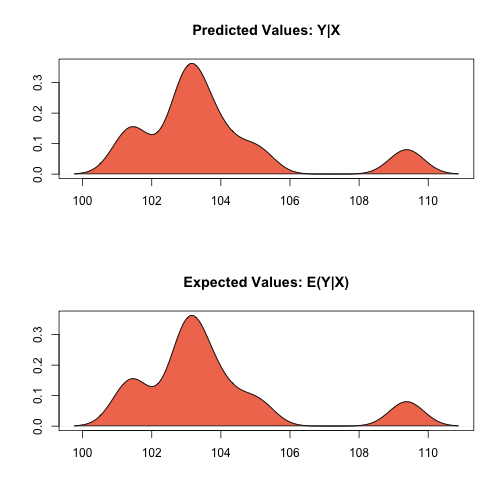
\includegraphics{QIs.png}
\caption{QIs}\end{figure}


\bigskip\hrule{}\bigskip


\emph{Plot of expected values across range of simulations:}


\chapter{Model Reference and Vignettes}
\label{vignette:vignettes}\label{vignette:model-reference-and-vignettes}\label{vignette::doc}
This section includes technical information on the models currently implemented in Zelig (5.0.1). This includes a reference with a list of supported models as well as individual model vignettes with detailed information on the model, quantities of interest and syntax.


\bigskip\hrule{}\bigskip



\section{Reference}
\label{vignette:reference}
The following models are currently supported in Zelig 5.0.1:
\begin{itemize}
\item {} 
\href{http://zeligproject.org/vignette.html\#zelig-exp}{Exponential Regression}: \code{zexp\$new()}

\item {} 
\href{http://zeligproject.org/vignette.html\#zelig-gamma}{Gamma Regression}: \code{zgamma()}

\item {} 
\href{http://zeligproject.org/vignette.html\#zelig-logit}{Logistic Regression}: \code{zlogit\$new()}

\item {} 
\href{http://zeligproject.org/vignette.html\#zelig-lognorm}{Log Normal Regression}: \code{zlognorm\$new()}

\item {} 
\href{http://zeligproject.org/vignette.html\#zelig-ls}{Least Squares Regression}: \code{zls\$new()}

\item {} 
\href{http://zeligproject.org/vignette.html\#zelig-exp}{Negative Binomial Regression}: \code{zbinom\$new()}

\item {} 
\href{http://zeligproject.org/vignette.html\#zelig-normal}{Normal Regression}: \code{znormal\$new()}

\item {} 
\href{http://zeligproject.org/vignette.html\#zelig-poisson}{Poisson Regression}: \code{zpoisson\$new()}

\item {} 
\href{http://zeligproject.org/vignette.html\#zelig-probit}{Probit Regression}: \code{zprobit\$new()}

\item {} 
\href{http://zeligproject.org/vignette.html\#zelig-relogit}{Rare Events Logistic Regression}: \code{zrelogit\$new()}

\item {} 
\href{http://zeligproject.org/vignette.html\#zelig-tobit}{Tobit Regression}: \code{ztobit\$new()}

\end{itemize}


\bigskip\hrule{}\bigskip



\section{zelig-exp}
\label{vignette:zelig-exp}
Exponential Regression for Duration Dependent Variables

Use the exponential duration regression model if you have a dependent
variable representing a duration (time until an event). The model
assumes a constant hazard rate for all events. The dependent variable
may be censored (for observations have not yet been completed when data
were collected).


\subsection{Syntax}
\label{vignette:syntax}
With reference classes:

\begin{Verbatim}[commandchars=\\\{\}]
z5 \PYG{o}{\PYGZlt{}\PYGZhy{}} zexp\PYG{o}{\PYGZdl{}}new\PYG{p}{(}\PYG{p}{)}
z5\PYG{o}{\PYGZdl{}}zelig\PYG{p}{(}Surv\PYG{p}{(}Y\PYG{p}{,} C\PYG{p}{)} \PYG{o}{\PYGZti{}} X\PYG{p}{,} data \PYG{o}{=} mydata\PYG{p}{)}
z5\PYG{o}{\PYGZdl{}}setx\PYG{p}{(}\PYG{p}{)}
z5\PYG{o}{\PYGZdl{}}sim\PYG{p}{(}\PYG{p}{)}
\end{Verbatim}

With the Zelig 4 compatibility wrappers:

\begin{Verbatim}[commandchars=\\\{\}]
z.out \PYG{o}{\PYGZlt{}\PYGZhy{}} zelig\PYG{p}{(}Surv\PYG{p}{(}Y\PYG{p}{,} C\PYG{p}{)} \PYG{o}{\PYGZti{}} X\PYG{p}{,} model \PYG{o}{=} \PYG{l+s}{\PYGZdq{}}\PYG{l+s}{exp\PYGZdq{}}\PYG{p}{,} data \PYG{o}{=} mydata\PYG{p}{)}
x.out \PYG{o}{\PYGZlt{}\PYGZhy{}} setx\PYG{p}{(}z.out\PYG{p}{)}
s.out \PYG{o}{\PYGZlt{}\PYGZhy{}} sim\PYG{p}{(}z.out\PYG{p}{,} x \PYG{o}{=} x.out\PYG{p}{)}
\end{Verbatim}

Exponential models require that the dependent variable be in the form
Surv(Y, C), where Y and C are vectors of length \(n\). For each
observation \(i\) in 1, …, \(n\), the value \(y_i\) is the
duration (lifetime, for example), and the associated \(c_i\) is a
binary variable such that \(c_i = 1\) if the duration is not
censored (\emph{e.g.}, the subject dies during the study) or \(c_i = 0\)
if the duration is censored (\emph{e.g.}, the subject is still alive at the
end of the study and is know to live at least as long as \(y_i\)).
If \(c_i\) is omitted, all Y are assumed to be completed; that is,
time defaults to 1 for all observations.


\subsection{Input Values}
\label{vignette:input-values}
In addition to the standard inputs, zelig() takes the following
additional options for exponential regression:
\begin{itemize}
\item {} 
robust: defaults to FALSE. If TRUE, zelig() computes robust standard
errors based on sandwich estimators (see and ) and the options
selected in cluster.

\item {} 
cluster: if robust = TRUE, you may select a variable to define groups
of correlated observations. Let x3 be a variable that consists of
either discrete numeric values, character strings, or factors that
define strata. Then

\end{itemize}

\begin{Verbatim}[commandchars=\\\{\}]
z.out \PYG{o}{\PYGZlt{}\PYGZhy{}} zelig\PYG{p}{(}y \PYG{o}{\PYGZti{}} x1 \PYG{o}{+} x2\PYG{p}{,} robust \PYG{o}{=} \PYG{k+kc}{TRUE}\PYG{p}{,} cluster \PYG{o}{=} \PYG{l+s}{\PYGZdq{}}\PYG{l+s}{x3\PYGZdq{}}\PYG{p}{,}
                        model \PYG{o}{=} \PYG{l+s}{\PYGZdq{}}\PYG{l+s}{exp\PYGZdq{}}\PYG{p}{,} data \PYG{o}{=} mydata\PYG{p}{)}
\end{Verbatim}

means that the observations can be correlated within the strata
defined by the variable x3, and that robust standard errors should be
calculated according to those clusters. If robust = TRUE but cluster
is not specified, zelig() assumes that each observation falls into
its own cluster.


\subsection{Example}
\label{vignette:example}
Attach the sample data:

\begin{Verbatim}[commandchars=\\\{\}]
data\PYG{p}{(}coalition\PYG{p}{)}
\end{Verbatim}

Estimate the model:

\begin{Verbatim}[commandchars=\\\{\}]
z.out \PYG{o}{\PYGZlt{}\PYGZhy{}} zelig\PYG{p}{(}Surv\PYG{p}{(}duration\PYG{p}{,} ciep12\PYG{p}{)} \PYG{o}{\PYGZti{}} fract \PYG{o}{+} numst2\PYG{p}{,} model \PYG{o}{=} \PYG{l+s}{\PYGZdq{}}\PYG{l+s}{exp\PYGZdq{}}\PYG{p}{,} data \PYG{o}{=} coalition\PYG{p}{)}
\end{Verbatim}

\begin{Verbatim}[commandchars=\\\{\}]
\PYG{c}{\PYGZsh{}\PYGZsh{} How to cite this model in Zelig:}
\PYG{c}{\PYGZsh{}\PYGZsh{}   Olivia Lau, Kosuke Imai, Gary King. 2011.}
\PYG{c}{\PYGZsh{}\PYGZsh{}   exp: Exponential Regression for Duration Dependent Variables}
\PYG{c}{\PYGZsh{}\PYGZsh{}   in Kosuke Imai, Gary King, and Olivia Lau, \PYGZdq{}Zelig: Everyone\PYGZsq{}s Statistical Software,\PYGZdq{}}
\PYG{c}{\PYGZsh{}\PYGZsh{}   http://datascience.iq.harvard.edu/zelig}
\end{Verbatim}

View the regression output:

\begin{Verbatim}[commandchars=\\\{\}]
summary\PYG{p}{(}z.out\PYG{p}{)}
\end{Verbatim}

\begin{Verbatim}[commandchars=\\\{\}]
\PYG{c}{\PYGZsh{}\PYGZsh{} Model: 1Call:}
\PYG{c}{\PYGZsh{}\PYGZsh{} survival::survreg(formula = Surv(duration, ciep12) \PYGZti{} fract +}
\PYG{c}{\PYGZsh{}\PYGZsh{}     numst2, data = ., dist = \PYGZdq{}exponential\PYGZdq{}, model = FALSE)}
\PYG{c}{\PYGZsh{}\PYGZsh{}}
\PYG{c}{\PYGZsh{}\PYGZsh{} Coefficients:}
\PYG{c}{\PYGZsh{}\PYGZsh{} (Intercept)       fract      numst2}
\PYG{c}{\PYGZsh{}\PYGZsh{}    5.535873   \PYGZhy{}0.003909    0.461179}
\PYG{c}{\PYGZsh{}\PYGZsh{}}
\PYG{c}{\PYGZsh{}\PYGZsh{} Scale fixed at 1}
\PYG{c}{\PYGZsh{}\PYGZsh{}}
\PYG{c}{\PYGZsh{}\PYGZsh{} Loglik(model)= \PYGZhy{}1077   Loglik(intercept only)= \PYGZhy{}1101}
\PYG{c}{\PYGZsh{}\PYGZsh{}  Chisq= 46.66 on 2 degrees of freedom, p= 7.4e\PYGZhy{}11}
\PYG{c}{\PYGZsh{}\PYGZsh{} n= 314}
\PYG{c}{\PYGZsh{}\PYGZsh{} Next step: Use \PYGZsq{}setx\PYGZsq{} method}
\end{Verbatim}

Set the baseline values (with the ruling coalition in the minority) and
the alternative values (with the ruling coalition in the majority) for
X:

\begin{Verbatim}[commandchars=\\\{\}]
x.low \PYG{o}{\PYGZlt{}\PYGZhy{}} setx\PYG{p}{(}z.out\PYG{p}{,} numst2 \PYG{o}{=} \PYG{l+m}{0}\PYG{p}{)}
x.high \PYG{o}{\PYGZlt{}\PYGZhy{}} setx\PYG{p}{(}z.out\PYG{p}{,} numst2 \PYG{o}{=} \PYG{l+m}{1}\PYG{p}{)}
\end{Verbatim}

Simulate expected values and first differences:

\begin{Verbatim}[commandchars=\\\{\}]
s.out \PYG{o}{\PYGZlt{}\PYGZhy{}} sim\PYG{p}{(}z.out\PYG{p}{,} x \PYG{o}{=} x.low\PYG{p}{,} x1 \PYG{o}{=} x.high\PYG{p}{)}
\end{Verbatim}

Summarize quantities of interest and produce some plots:

\begin{Verbatim}[commandchars=\\\{\}]
summary\PYG{p}{(}s.out\PYG{p}{)}
\end{Verbatim}

\begin{Verbatim}[commandchars=\\\{\}]
\PYG{c}{\PYGZsh{}\PYGZsh{}}
\PYG{c}{\PYGZsh{}\PYGZsh{}  sim x :}
\PYG{c}{\PYGZsh{}\PYGZsh{}  \PYGZhy{}\PYGZhy{}\PYGZhy{}\PYGZhy{}\PYGZhy{}}
\PYG{c}{\PYGZsh{}\PYGZsh{} ev}
\PYG{c}{\PYGZsh{}\PYGZsh{}    mean    sd   50\PYGZpc{}  2.5\PYGZpc{} 97.5\PYGZpc{}}
\PYG{c}{\PYGZsh{}\PYGZsh{} 1 15.32 1.451 15.26 12.74 18.47}
\PYG{c}{\PYGZsh{}\PYGZsh{} pv}
\PYG{c}{\PYGZsh{}\PYGZsh{}       mean    sd   50\PYGZpc{}  2.5\PYGZpc{} 97.5\PYGZpc{}}
\PYG{c}{\PYGZsh{}\PYGZsh{} [1,] 14.45 13.54 11.23 0.369 50.85}
\PYG{c}{\PYGZsh{}\PYGZsh{}}
\PYG{c}{\PYGZsh{}\PYGZsh{}  sim x1 :}
\PYG{c}{\PYGZsh{}\PYGZsh{}  \PYGZhy{}\PYGZhy{}\PYGZhy{}\PYGZhy{}\PYGZhy{}}
\PYG{c}{\PYGZsh{}\PYGZsh{} ev}
\PYG{c}{\PYGZsh{}\PYGZsh{}    mean    sd   50\PYGZpc{}  2.5\PYGZpc{} 97.5\PYGZpc{}}
\PYG{c}{\PYGZsh{}\PYGZsh{} 1 24.29 1.883 24.27 20.77 28.19}
\PYG{c}{\PYGZsh{}\PYGZsh{} pv}
\PYG{c}{\PYGZsh{}\PYGZsh{}       mean    sd   50\PYGZpc{}   2.5\PYGZpc{} 97.5\PYGZpc{}}
\PYG{c}{\PYGZsh{}\PYGZsh{} [1,] 25.29 23.86 18.05 0.6137 88.22}
\PYG{c}{\PYGZsh{}\PYGZsh{} fd}
\PYG{c}{\PYGZsh{}\PYGZsh{}    mean    sd   50\PYGZpc{} 2.5\PYGZpc{} 97.5\PYGZpc{}}
\PYG{c}{\PYGZsh{}\PYGZsh{} 1 8.971 2.405 8.952  4.4 13.88}
\end{Verbatim}

\begin{Verbatim}[commandchars=\\\{\}]
plot\PYG{p}{(}s.out\PYG{p}{)}
\end{Verbatim}
\begin{figure}[htbp]
\centering
\capstart

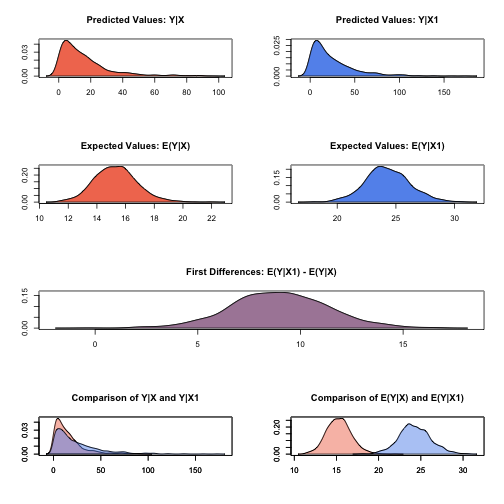
\includegraphics{Zelig-exp.png}
\caption{Zelig-exp}\end{figure}


\subsection{Model}
\label{vignette:model}
Let \(Y_i^*\) be the survival time for observation \(i\). This
variable might be censored for some observations at a fixed time
\(y_c\) such that the fully observed dependent variable,
\(Y_i\), is defined as
\begin{gather}
\begin{split}Y_i = \left\{ \begin{array}{ll}
      Y_i^* & \textrm{if }Y_i^* \leq y_c \\
      y_c & \textrm{if }Y_i^* > y_c \\
    \end{array} \right.\end{split}\notag
\end{gather}\begin{itemize}
\item {} 
The \emph{stochastic component} is described by the distribution of the
partially observed variable \(Y^*\). We assume \(Y_i^*\)
follows the exponential distribution whose density function is given
by
\begin{gather}
\begin{split}f(y_i^*\mid \lambda_i) = \frac{1}{\lambda_i} \exp\left(-\frac{y_i^*}{\lambda_i}\right)\end{split}\notag
\end{gather}
for \(y_i^*\ge 0\) and \(\lambda_i>0\). The mean of this
distribution is \(\lambda_i\).

In addition, survival models like the exponential have three
additional properties. The hazard function \(h(t)\) measures the
probability of not surviving past time \(t\) given survival up to
\(t\). In general, the hazard function is equal to
\(f(t)/S(t)\) where the survival function
\(S(t) = 1 - \int_{0}^t f(s) ds\) represents the fraction still
surviving at time \(t\). The cumulative hazard function
\(H(t)\) describes the probability of dying before time
\(t\). In general,
\(H(t)= \int_{0}^{t} h(s) ds = -\log S(t)\). In the case of the
exponential model,
\begin{gather}
\begin{split}\begin{aligned}
h(t) &=& \frac{1}{\lambda_i} \\
S(t) &=& \exp\left( -\frac{t}{\lambda_i} \right) \\
H(t) &=& \frac{t}{\lambda_i}\end{aligned}\end{split}\notag
\end{gather}
For the exponential model, the hazard function \(h(t)\) is
constant over time. The Weibull model and lognormal models allow the
hazard function to vary as a function of elapsed time (see and
respectively).

\item {} 
The \emph{systematic component} \(\lambda_i\) is modeled as
\begin{gather}
\begin{split}\lambda_i = \exp(x_i \beta),\end{split}\notag
\end{gather}
where \(x_i\) is the vector of explanatory variables, and
\(\beta\) is the vector of coefficients.

\end{itemize}


\subsection{Quantities of Interest}
\label{vignette:quantities-of-interest}\begin{itemize}
\item {} 
The expected values (qi\$ev) for the exponential model are simulations
of the expected duration given \(x_i\) and draws of \(\beta\)
from its posterior,
\begin{gather}
\begin{split}E(Y) = \lambda_i = \exp(x_i \beta).\end{split}\notag
\end{gather}
\item {} 
The predicted values (qi\$pr) are draws from the exponential
distribution with rate equal to the expected value.

\item {} 
The first difference (or difference in expected values, qi\$ev.diff),
is
\begin{gather}
\begin{split}\textrm{FD} \; = \; E(Y \mid x_1) - E(Y \mid x),\end{split}\notag
\end{gather}
where \(x\) and \(x_1\) are different vectors of values for
the explanatory variables.

\item {} 
In conditional prediction models, the average expected treatment
effect (att.ev) for the treatment group is
\begin{gather}
\begin{split}\frac{1}{\sum_{i=1}^n t_i}\sum_{i:t_i=1}^n \left\{ Y_i(t_i=1) - E[Y_i(t_i=0)]
  \right\},\end{split}\notag
\end{gather}
where \(t_i\) is a binary explanatory variable defining the
treatment (\(t_i=1\)) and control (\(t_i=0\)) groups. When
\(Y_i(t_i=1)\) is censored rather than observed, we replace it
with a simulation from the model given available knowledge of the
censoring process. Variation in the simulations is due to two
factors: uncertainty in the imputation process for censored
\(y_i^*\) and uncertainty in simulating \(E[Y_i(t_i=0)]\),
the counterfactual expected value of \(Y_i\) for observations in
the treatment group, under the assumption that everything stays the
same except that the treatment indicator is switched to
\(t_i=0\).

\item {} 
In conditional prediction models, the average predicted treatment
effect (att.pr) for the treatment group is
\begin{gather}
\begin{split}\frac{1}{\sum_{i=1}^n t_i}\sum_{i:t_i=1}^n \left\{ Y_i(t_i=1) -
  \widehat{Y_i(t_i=0)} \right\},\end{split}\notag
\end{gather}
where \(t_i\) is a binary explanatory variable defining the
treatment (\(t_i=1\)) and control (\(t_i=0\)) groups. When
\(Y_i(t_i=1)\) is censored rather than observed, we replace it
with a simulation from the model given available knowledge of the
censoring process. Variation in the simulations is due to two
factors: uncertainty in the imputation process for censored
\(y_i^*\) and uncertainty in simulating
\(\widehat{Y_i(t_i=0)}\), the counterfactual predicted value of
\(Y_i\) for observations in the treatment group, under the
assumption that everything stays the same except that the treatment
indicator is switched to \(t_i=0\).

\end{itemize}


\subsection{Output Values}
\label{vignette:output-values}
The output of each Zelig command contains useful information which you
may view. For example, if you run
\code{z.out \textless{}- zelig(Surv(Y, C) \textasciitilde{} X, model = exp, data)}, then you may
examine the available information in \code{z.out} by using
\code{names(z.out)}, see the coefficients by using z.out\$coefficients, and
a default summary of information through \code{summary(z.out)}.


\subsection{See also}
\label{vignette:see-also}
The exponential function is part of the survival library by Terry
Therneau, ported to R by Thomas Lumley. Advanced users may wish to refer
to \code{help(survfit)} in the survival library.


\bigskip\hrule{}\bigskip



\section{zelig-gamma}
\label{vignette:zelig-gamma}
Gamma Regression for Continuous, Positive Dependent Variables

Use the gamma regression model if you have a positive-valued dependent
variable such as the number of years a parliamentary cabinet endures, or
the seconds you can stay airborne while jumping. The gamma distribution
assumes that all waiting times are complete by the end of the study
(censoring is not allowed).


\subsection{Syntax}
\label{vignette:id1}
With reference classes:

\begin{Verbatim}[commandchars=\\\{\}]
z5 \PYG{o}{\PYGZlt{}\PYGZhy{}} zgamma\PYG{o}{\PYGZdl{}}new\PYG{p}{(}\PYG{p}{)}
z5\PYG{o}{\PYGZdl{}}zelig\PYG{p}{(}Y \PYG{o}{\PYGZti{}} X1 \PYG{o}{+} X \PYG{o}{\PYGZti{}} X\PYG{p}{,} data \PYG{o}{=} mydata\PYG{p}{)}
z5\PYG{o}{\PYGZdl{}}setx\PYG{p}{(}\PYG{p}{)}
z5\PYG{o}{\PYGZdl{}}sim\PYG{p}{(}\PYG{p}{)}
\end{Verbatim}

With the Zelig 4 compatibility wrappers:

\begin{Verbatim}[commandchars=\\\{\}]
z.out \PYG{o}{\PYGZlt{}\PYGZhy{}} zelig\PYG{p}{(}Y \PYG{o}{\PYGZti{}} X1 \PYG{o}{+} X2\PYG{p}{,} model \PYG{o}{=} \PYG{l+s}{\PYGZdq{}}\PYG{l+s}{gamma\PYGZdq{}}\PYG{p}{,} data \PYG{o}{=} mydata\PYG{p}{)}
x.out \PYG{o}{\PYGZlt{}\PYGZhy{}} setx\PYG{p}{(}z.out\PYG{p}{)}
s.out \PYG{o}{\PYGZlt{}\PYGZhy{}} sim\PYG{p}{(}z.out\PYG{p}{,} x \PYG{o}{=} x.out\PYG{p}{,} x1 \PYG{o}{=} \PYG{k+kc}{NULL}\PYG{p}{)}
\end{Verbatim}


\subsection{Example}
\label{vignette:id2}
Attach the sample data:

\begin{Verbatim}[commandchars=\\\{\}]
data\PYG{p}{(}coalition\PYG{p}{)}
\end{Verbatim}

Estimate the model:

\begin{Verbatim}[commandchars=\\\{\}]
z.out \PYG{o}{\PYGZlt{}\PYGZhy{}} zelig\PYG{p}{(}duration \PYG{o}{\PYGZti{}} fract \PYG{o}{+} numst2\PYG{p}{,} model \PYG{o}{=} \PYG{l+s}{\PYGZdq{}}\PYG{l+s}{gamma\PYGZdq{}}\PYG{p}{,} data \PYG{o}{=} coalition\PYG{p}{)}
\end{Verbatim}

\begin{Verbatim}[commandchars=\\\{\}]
\PYG{c}{\PYGZsh{}\PYGZsh{} How to cite this model in Zelig:}
\PYG{c}{\PYGZsh{}\PYGZsh{}   Kosuke Imai, Gary King, Olivia Lau. 2007.}
\PYG{c}{\PYGZsh{}\PYGZsh{}   gamma: Gamma Regression for Continuous, Positive Dependent Variables}
\PYG{c}{\PYGZsh{}\PYGZsh{}   in Kosuke Imai, Gary King, and Olivia Lau, \PYGZdq{}Zelig: Everyone\PYGZsq{}s Statistical Software,\PYGZdq{}}
\PYG{c}{\PYGZsh{}\PYGZsh{}   http://datascience.iq.harvard.edu/zelig}
\end{Verbatim}

View the regression output:

\begin{Verbatim}[commandchars=\\\{\}]
summary\PYG{p}{(}z.out\PYG{p}{)}
\end{Verbatim}

\begin{Verbatim}[commandchars=\\\{\}]
\PYG{c}{\PYGZsh{}\PYGZsh{} Model: 1}
\PYG{c}{\PYGZsh{}\PYGZsh{} Call:  stats::glm(formula = duration \PYGZti{} fract + numst2, family = Gamma(\PYGZdq{}inverse\PYGZdq{}),}
\PYG{c}{\PYGZsh{}\PYGZsh{}     data = .)}
\PYG{c}{\PYGZsh{}\PYGZsh{}}
\PYG{c}{\PYGZsh{}\PYGZsh{} Coefficients:}
\PYG{c}{\PYGZsh{}\PYGZsh{} (Intercept)        fract       numst2}
\PYG{c}{\PYGZsh{}\PYGZsh{}   \PYGZhy{}0.012960     0.000115    \PYGZhy{}0.017387}
\PYG{c}{\PYGZsh{}\PYGZsh{}}
\PYG{c}{\PYGZsh{}\PYGZsh{} Degrees of Freedom: 313 Total (i.e. Null);  311 Residual}
\PYG{c}{\PYGZsh{}\PYGZsh{} Null Deviance:       301}
\PYG{c}{\PYGZsh{}\PYGZsh{} Residual Deviance: 272   AIC: 2430}
\PYG{c}{\PYGZsh{}\PYGZsh{} Next step: Use \PYGZsq{}setx\PYGZsq{} method}
\end{Verbatim}

Set the baseline values (with the ruling coalition in the minority) and
the alternative values (with the ruling coalition in the majority) for
X:

\begin{Verbatim}[commandchars=\\\{\}]
x.low \PYG{o}{\PYGZlt{}\PYGZhy{}} setx\PYG{p}{(}z.out\PYG{p}{,} numst2 \PYG{o}{=} \PYG{l+m}{0}\PYG{p}{)}
x.high \PYG{o}{\PYGZlt{}\PYGZhy{}} setx\PYG{p}{(}z.out\PYG{p}{,} numst2 \PYG{o}{=} \PYG{l+m}{1}\PYG{p}{)}
\end{Verbatim}

Simulate expected values (qi\$ev) and first differences (qi\$fd):

\begin{Verbatim}[commandchars=\\\{\}]
s.out \PYG{o}{\PYGZlt{}\PYGZhy{}} sim\PYG{p}{(}z.out\PYG{p}{,} x \PYG{o}{=} x.low\PYG{p}{,} x1 \PYG{o}{=} x.high\PYG{p}{)}
\end{Verbatim}

\begin{Verbatim}[commandchars=\\\{\}]
summary\PYG{p}{(}s.out\PYG{p}{)}
\end{Verbatim}

\begin{Verbatim}[commandchars=\\\{\}]
\PYG{c}{\PYGZsh{}\PYGZsh{}}
\PYG{c}{\PYGZsh{}\PYGZsh{}  sim x :}
\PYG{c}{\PYGZsh{}\PYGZsh{}  \PYGZhy{}\PYGZhy{}\PYGZhy{}\PYGZhy{}\PYGZhy{}}
\PYG{c}{\PYGZsh{}\PYGZsh{} ev}
\PYG{c}{\PYGZsh{}\PYGZsh{}       mean    sd   50\PYGZpc{}  2.5\PYGZpc{} 97.5\PYGZpc{}}
\PYG{c}{\PYGZsh{}\PYGZsh{} [1,] 14.45 1.074 14.37 12.64 16.88}
\PYG{c}{\PYGZsh{}\PYGZsh{} pv}
\PYG{c}{\PYGZsh{}\PYGZsh{}       mean    sd   50\PYGZpc{}   2.5\PYGZpc{} 97.5\PYGZpc{}}
\PYG{c}{\PYGZsh{}\PYGZsh{} [1,] 14.02 12.68 10.72 0.6749 46.73}
\PYG{c}{\PYGZsh{}\PYGZsh{}}
\PYG{c}{\PYGZsh{}\PYGZsh{}  sim x1 :}
\PYG{c}{\PYGZsh{}\PYGZsh{}  \PYGZhy{}\PYGZhy{}\PYGZhy{}\PYGZhy{}\PYGZhy{}}
\PYG{c}{\PYGZsh{}\PYGZsh{} ev}
\PYG{c}{\PYGZsh{}\PYGZsh{}       mean    sd   50\PYGZpc{}  2.5\PYGZpc{} 97.5\PYGZpc{}}
\PYG{c}{\PYGZsh{}\PYGZsh{} [1,] 19.21 1.096 19.13 17.32 21.51}
\PYG{c}{\PYGZsh{}\PYGZsh{} pv}
\PYG{c}{\PYGZsh{}\PYGZsh{}       mean    sd   50\PYGZpc{}  2.5\PYGZpc{} 97.5\PYGZpc{}}
\PYG{c}{\PYGZsh{}\PYGZsh{} [1,] 19.35 17.51 14.95 1.229 65.31}
\PYG{c}{\PYGZsh{}\PYGZsh{} fd}
\PYG{c}{\PYGZsh{}\PYGZsh{}       mean    sd   50\PYGZpc{}  2.5\PYGZpc{} 97.5\PYGZpc{}}
\PYG{c}{\PYGZsh{}\PYGZsh{} [1,] 4.761 1.539 4.714 1.732 7.879}
\end{Verbatim}

\begin{Verbatim}[commandchars=\\\{\}]
plot\PYG{p}{(}s.out\PYG{p}{)}
\end{Verbatim}
\begin{figure}[htbp]
\centering
\capstart

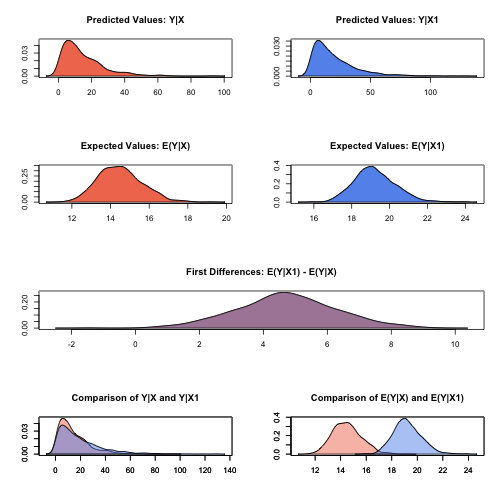
\includegraphics{Zelig-gamma.png}
\caption{Zelig-gamma}\end{figure}


\subsection{Model}
\label{vignette:id3}\begin{itemize}
\item {} 
The Gamma distribution with scale parameter \(\alpha\) has a
\emph{stochastic component}:
\begin{gather}
\begin{split}\begin{aligned}
Y &\sim& \textrm{Gamma}(y_i \mid \lambda_i, \alpha) \\
f(y)  &=& \frac{1}{\alpha^{\lambda_i} \, \Gamma \lambda_i} \, y_i^{\lambda_i
  - 1} \exp -\left\{ \frac{y_i}{\alpha} \right\}\end{aligned}\end{split}\notag
\end{gather}
\begin{DUlineblock}{0em}
\item[] for \(\alpha, \lambda_i, y_i > 0\).
\end{DUlineblock}

\item {} 
The \emph{systematic component} is given by
\begin{gather}
\begin{split}\lambda_i = \frac{1}{x_i \beta}\end{split}\notag
\end{gather}
\end{itemize}


\subsection{Quantities of Interest}
\label{vignette:id4}\begin{itemize}
\item {} 
The expected values (qi\$ev) are simulations of the mean of the
stochastic component given draws of \(\alpha\) and \(\beta\)
from their posteriors:
\begin{gather}
\begin{split}E(Y) = \alpha \lambda_i.\end{split}\notag
\end{gather}
\item {} 
The predicted values (qi\$pr) are draws from the gamma distribution
for each given set of parameters \((\alpha, \lambda_i)\).

\item {} 
If x1 is specified, sim() also returns the differences in the
expected values (qi\$fd),
\begin{gather}
\begin{split}E(Y \mid x_1) -
  E(Y \mid x)\end{split}\notag
\end{gather}
.

\item {} 
In conditional prediction models, the average expected treatment
effect (att.ev) for the treatment group is
\begin{gather}
\begin{split}\frac{1}{\sum_{i=1}^n t_i}\sum_{i:t_i=1}^n \left\{ Y_i(t_i=1) -
      E[Y_i(t_i=0)] \right\},\end{split}\notag
\end{gather}
where \(t_i\) is a binary explanatory variable defining the
treatment (\(t_i=1\)) and control (\(t_i=0\)) groups.
Variation in the simulations are due to uncertainty in simulating
\(E[Y_i(t_i=0)]\), the counterfactual expected value of
\(Y_i\) for observations in the treatment group, under the
assumption that everything stays the same except that the treatment
indicator is switched to \(t_i=0\).

\item {} 
In conditional prediction models, the average predicted treatment
effect (att.pr) for the treatment group is
\begin{gather}
\begin{split}\frac{1}{\sum_{i=1}^n t_i}\sum_{i:t_i=1}^n \left\{ Y_i(t_i=1) -
      \widehat{Y_i(t_i=0)} \right\},\end{split}\notag
\end{gather}
where \(t_i\) is a binary explanatory variable defining the
treatment (\(t_i=1\)) and control (\(t_i=0\)) groups.
Variation in the simulations are due to uncertainty in simulating
\(\widehat{Y_i(t_i=0)}\), the counterfactual predicted value of
\(Y_i\) for observations in the treatment group, under the
assumption that everything stays the same except that the treatment
indicator is switched to \(t_i=0\).

\end{itemize}


\subsection{Output Values}
\label{vignette:id5}
The output of each Zelig command contains useful information which you
may view. For example, if you run
\code{z.out \textless{}- zelig(y \textasciitilde{} x, model = gamma, data)}, then you may examine the
available information in \code{z.out} by using \code{names(z.out)}, see the
coefficients by using z.out\$coefficients, and a default summary of
information through \code{summary(z.out)}.


\subsection{See also}
\label{vignette:id6}
The gamma model is part of the stats package. Advanced users may
wish to refer to \code{help(glm)} and \code{help(family)}.


\bigskip\hrule{}\bigskip



\section{zelig-logit}
\label{vignette:zelig-logit}
Logistic Regression for Dichotomous Dependent Variables

Logistic regression specifies a dichotomous dependent variable as a
function of a set of explanatory variables.


\subsection{Syntax}
\label{vignette:id7}
With reference classes:

\begin{Verbatim}[commandchars=\\\{\}]
z5 \PYG{o}{\PYGZlt{}\PYGZhy{}} zlogit\PYG{o}{\PYGZdl{}}new\PYG{p}{(}\PYG{p}{)}
z5\PYG{o}{\PYGZdl{}}zelig\PYG{p}{(}Y \PYG{o}{\PYGZti{}} X1 \PYG{o}{+} X \PYG{o}{\PYGZti{}} X\PYG{p}{,} data \PYG{o}{=} mydata\PYG{p}{)}
z5\PYG{o}{\PYGZdl{}}setx\PYG{p}{(}\PYG{p}{)}
z5\PYG{o}{\PYGZdl{}}sim\PYG{p}{(}\PYG{p}{)}
\end{Verbatim}

With the Zelig 4 compatibility wrappers:

\begin{Verbatim}[commandchars=\\\{\}]
z.out \PYG{o}{\PYGZlt{}\PYGZhy{}} zelig\PYG{p}{(}Y \PYG{o}{\PYGZti{}} X1 \PYG{o}{+} X2\PYG{p}{,} model \PYG{o}{=} \PYG{l+s}{\PYGZdq{}}\PYG{l+s}{logit\PYGZdq{}}\PYG{p}{,} data \PYG{o}{=} mydata\PYG{p}{)}
x.out \PYG{o}{\PYGZlt{}\PYGZhy{}} setx\PYG{p}{(}z.out\PYG{p}{)}
s.out \PYG{o}{\PYGZlt{}\PYGZhy{}} sim\PYG{p}{(}z.out\PYG{p}{,} x \PYG{o}{=} x.out\PYG{p}{,} x1 \PYG{o}{=} \PYG{k+kc}{NULL}\PYG{p}{)}
\end{Verbatim}


\subsection{Examples}
\label{vignette:examples}

\subsubsection{Basic Example}
\label{vignette:basic-example}
Attaching the sample turnout dataset:

\begin{Verbatim}[commandchars=\\\{\}]
data\PYG{p}{(}turnout\PYG{p}{)}
\end{Verbatim}

Estimating parameter values for the logistic regression:

\begin{Verbatim}[commandchars=\\\{\}]
z.out1 \PYG{o}{\PYGZlt{}\PYGZhy{}} zelig\PYG{p}{(}vote \PYG{o}{\PYGZti{}} age \PYG{o}{+} race\PYG{p}{,} model \PYG{o}{=} \PYG{l+s}{\PYGZdq{}}\PYG{l+s}{logit\PYGZdq{}}\PYG{p}{,} data \PYG{o}{=} turnout\PYG{p}{)}
\end{Verbatim}

\begin{Verbatim}[commandchars=\\\{\}]
\PYG{c}{\PYGZsh{}\PYGZsh{} How to cite this model in Zelig:}
\PYG{c}{\PYGZsh{}\PYGZsh{}   Kosuke Imai, Gary King, Olivia Lau. 2007.}
\PYG{c}{\PYGZsh{}\PYGZsh{}   logit: Logistic Regression for Dichotomous Dependent Variables}
\PYG{c}{\PYGZsh{}\PYGZsh{}   in Kosuke Imai, Gary King, and Olivia Lau, \PYGZdq{}Zelig: Everyone\PYGZsq{}s Statistical Software,\PYGZdq{}}
\PYG{c}{\PYGZsh{}\PYGZsh{}   http://datascience.iq.harvard.edu/zelig}
\end{Verbatim}

Setting values for the explanatory variables:

\begin{Verbatim}[commandchars=\\\{\}]
x.out1 \PYG{o}{\PYGZlt{}\PYGZhy{}} setx\PYG{p}{(}z.out1\PYG{p}{,} age \PYG{o}{=} \PYG{l+m}{36}\PYG{p}{,} race \PYG{o}{=} \PYG{l+s}{\PYGZdq{}}\PYG{l+s}{white\PYGZdq{}}\PYG{p}{)}
\end{Verbatim}

Simulating quantities of interest from the posterior distribution.

\begin{Verbatim}[commandchars=\\\{\}]
s.out1 \PYG{o}{\PYGZlt{}\PYGZhy{}} sim\PYG{p}{(}z.out1\PYG{p}{,} x \PYG{o}{=} x.out1\PYG{p}{)}
\end{Verbatim}

\begin{Verbatim}[commandchars=\\\{\}]
summary\PYG{p}{(}s.out1\PYG{p}{)}
\end{Verbatim}

\begin{Verbatim}[commandchars=\\\{\}]
\PYG{c}{\PYGZsh{}\PYGZsh{}}
\PYG{c}{\PYGZsh{}\PYGZsh{}  sim x :}
\PYG{c}{\PYGZsh{}\PYGZsh{}  \PYGZhy{}\PYGZhy{}\PYGZhy{}\PYGZhy{}\PYGZhy{}}
\PYG{c}{\PYGZsh{}\PYGZsh{} ev}
\PYG{c}{\PYGZsh{}\PYGZsh{}        mean      sd    50\PYGZpc{}   2.5\PYGZpc{} 97.5\PYGZpc{}}
\PYG{c}{\PYGZsh{}\PYGZsh{} [1,] 0.7484 0.01172 0.7491 0.7249  0.77}
\PYG{c}{\PYGZsh{}\PYGZsh{} pv}
\PYG{c}{\PYGZsh{}\PYGZsh{}          0     1}
\PYG{c}{\PYGZsh{}\PYGZsh{} [1,] 0.225 0.775}
\end{Verbatim}

\begin{Verbatim}[commandchars=\\\{\}]
plot\PYG{p}{(}s.out1\PYG{p}{)}
\end{Verbatim}
\begin{figure}[htbp]
\centering
\capstart

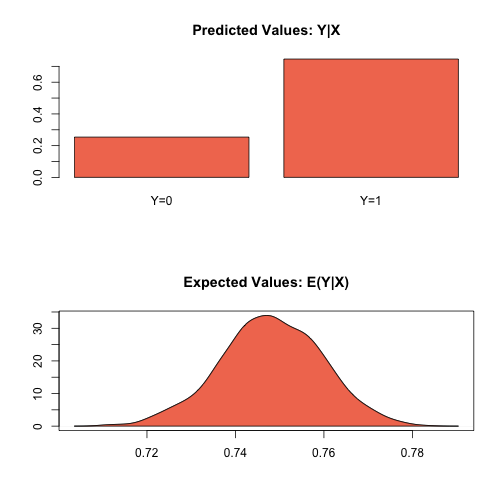
\includegraphics{Zelig-logit-1.png}
\caption{Zelig-logit-1}\end{figure}


\subsubsection{Simulating First Differences}
\label{vignette:simulating-first-differences}
Estimating the risk difference (and risk ratio) between low education
(25th percentile) and high education (75th percentile) while all the
other variables held at their default values.

\begin{Verbatim}[commandchars=\\\{\}]
z.out2 \PYG{o}{\PYGZlt{}\PYGZhy{}} zelig\PYG{p}{(}vote \PYG{o}{\PYGZti{}} race \PYG{o}{+} educate\PYG{p}{,} model \PYG{o}{=} \PYG{l+s}{\PYGZdq{}}\PYG{l+s}{logit\PYGZdq{}}\PYG{p}{,} data \PYG{o}{=} turnout\PYG{p}{)}
\end{Verbatim}

\begin{Verbatim}[commandchars=\\\{\}]
\PYG{c}{\PYGZsh{}\PYGZsh{} How to cite this model in Zelig:}
\PYG{c}{\PYGZsh{}\PYGZsh{}   Kosuke Imai, Gary King, Olivia Lau. 2007.}
\PYG{c}{\PYGZsh{}\PYGZsh{}   logit: Logistic Regression for Dichotomous Dependent Variables}
\PYG{c}{\PYGZsh{}\PYGZsh{}   in Kosuke Imai, Gary King, and Olivia Lau, \PYGZdq{}Zelig: Everyone\PYGZsq{}s Statistical Software,\PYGZdq{}}
\PYG{c}{\PYGZsh{}\PYGZsh{}   http://datascience.iq.harvard.edu/zelig}
\end{Verbatim}

\begin{Verbatim}[commandchars=\\\{\}]
x.high \PYG{o}{\PYGZlt{}\PYGZhy{}} setx\PYG{p}{(}z.out2\PYG{p}{,} educate \PYG{o}{=} quantile\PYG{p}{(}turnout\PYG{o}{\PYGZdl{}}educate\PYG{p}{,} prob \PYG{o}{=} \PYG{l+m}{0.75}\PYG{p}{)}\PYG{p}{)}
x.low \PYG{o}{\PYGZlt{}\PYGZhy{}} setx\PYG{p}{(}z.out2\PYG{p}{,} educate \PYG{o}{=} quantile\PYG{p}{(}turnout\PYG{o}{\PYGZdl{}}educate\PYG{p}{,} prob \PYG{o}{=} \PYG{l+m}{0.25}\PYG{p}{)}\PYG{p}{)}
s.out2 \PYG{o}{\PYGZlt{}\PYGZhy{}} sim\PYG{p}{(}z.out2\PYG{p}{,} x \PYG{o}{=} x.high\PYG{p}{,} x1 \PYG{o}{=} x.low\PYG{p}{)}
summary\PYG{p}{(}s.out2\PYG{p}{)}
\end{Verbatim}

\begin{Verbatim}[commandchars=\\\{\}]
\PYG{c}{\PYGZsh{}\PYGZsh{}}
\PYG{c}{\PYGZsh{}\PYGZsh{}  sim x :}
\PYG{c}{\PYGZsh{}\PYGZsh{}  \PYGZhy{}\PYGZhy{}\PYGZhy{}\PYGZhy{}\PYGZhy{}}
\PYG{c}{\PYGZsh{}\PYGZsh{} ev}
\PYG{c}{\PYGZsh{}\PYGZsh{}       mean      sd    50\PYGZpc{}   2.5\PYGZpc{}  97.5\PYGZpc{}}
\PYG{c}{\PYGZsh{}\PYGZsh{} [1,] 0.823 0.01053 0.8235 0.8011 0.8434}
\PYG{c}{\PYGZsh{}\PYGZsh{} pv}
\PYG{c}{\PYGZsh{}\PYGZsh{}         0    1}
\PYG{c}{\PYGZsh{}\PYGZsh{} [1,] 0.18 0.82}
\PYG{c}{\PYGZsh{}\PYGZsh{}}
\PYG{c}{\PYGZsh{}\PYGZsh{}  sim x1 :}
\PYG{c}{\PYGZsh{}\PYGZsh{}  \PYGZhy{}\PYGZhy{}\PYGZhy{}\PYGZhy{}\PYGZhy{}}
\PYG{c}{\PYGZsh{}\PYGZsh{} ev}
\PYG{c}{\PYGZsh{}\PYGZsh{}        mean      sd    50\PYGZpc{}   2.5\PYGZpc{}  97.5\PYGZpc{}}
\PYG{c}{\PYGZsh{}\PYGZsh{} [1,] 0.7095 0.01314 0.7096 0.6836 0.7337}
\PYG{c}{\PYGZsh{}\PYGZsh{} pv}
\PYG{c}{\PYGZsh{}\PYGZsh{}          0     1}
\PYG{c}{\PYGZsh{}\PYGZsh{} [1,] 0.295 0.705}
\PYG{c}{\PYGZsh{}\PYGZsh{} fd}
\PYG{c}{\PYGZsh{}\PYGZsh{}         mean      sd     50\PYGZpc{}    2.5\PYGZpc{}    97.5\PYGZpc{}}
\PYG{c}{\PYGZsh{}\PYGZsh{} [1,] \PYGZhy{}0.1134 0.01184 \PYGZhy{}0.1139 \PYGZhy{}0.1355 \PYGZhy{}0.09111}
\end{Verbatim}

\begin{Verbatim}[commandchars=\\\{\}]
plot\PYG{p}{(}s.out2\PYG{p}{)}
\end{Verbatim}
\begin{figure}[htbp]
\centering
\capstart

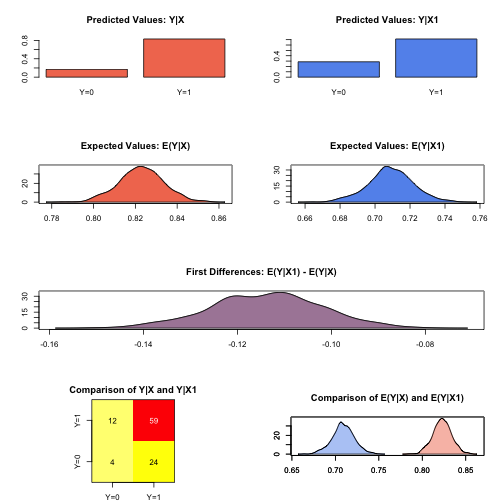
\includegraphics{Zelig-logit-2.png}
\caption{Zelig-logit-2}\end{figure}


\subsection{Model}
\label{vignette:id8}
Let \(Y_i\) be the binary dependent variable for observation
\(i\) which takes the value of either 0 or 1.
\begin{itemize}
\item {} 
The \emph{stochastic component} is given by
\begin{gather}
\begin{split}\begin{aligned}
Y_i &\sim& \textrm{Bernoulli}(y_i \mid \pi_i) \\
    &=& \pi_i^{y_i} (1-\pi_i)^{1-y_i}\end{aligned}\end{split}\notag
\end{gather}
where \(\pi_i=\Pr(Y_i=1)\).

\item {} 
The \emph{systematic component} is given by:
\begin{gather}
\begin{split}\pi_i \; = \; \frac{1}{1 + \exp(-x_i \beta)}.\end{split}\notag
\end{gather}
where \(x_i\) is the vector of \(k\) explanatory variables
for observation \(i\) and \(\beta\) is the vector of
coefficients.

\end{itemize}


\subsection{Quantities of Interest}
\label{vignette:id9}\begin{itemize}
\item {} 
The expected values (qi\$ev) for the logit model are simulations of
the predicted probability of a success:
\begin{gather}
\begin{split}E(Y) =
  \pi_i= \frac{1}{1 + \exp(-x_i \beta)},\end{split}\notag
\end{gather}
given draws of \(\beta\) from its sampling distribution.

\item {} 
The predicted values (qi\$pr) are draws from the Binomial distribution
with mean equal to the simulated expected value \(\pi_i\).

\item {} 
The first difference (qi\$fd) for the logit model is defined as
\begin{gather}
\begin{split}\textrm{FD} = \Pr(Y = 1 \mid x_1) - \Pr(Y = 1 \mid x).\end{split}\notag
\end{gather}
\item {} 
The risk ratio (qi\$rr) is defined as
\begin{gather}
\begin{split}\textrm{RR} = \Pr(Y = 1 \mid x_1) \ / \ \Pr(Y = 1 \mid x).\end{split}\notag
\end{gather}
\item {} 
In conditional prediction models, the average expected treatment
effect (att.ev) for the treatment group is
\begin{gather}
\begin{split}\frac{1}{\sum_{i=1}^n t_i}\sum_{i:t_i=1}^n \left\{ Y_i(t_i=1) -
      E[Y_i(t_i=0)] \right\},\end{split}\notag
\end{gather}
where \(t_i\) is a binary explanatory variable defining the
treatment (\(t_i=1\)) and control (\(t_i=0\)) groups.
Variation in the simulations are due to uncertainty in simulating
\(E[Y_i(t_i=0)]\), the counterfactual expected value of
\(Y_i\) for observations in the treatment group, under the
assumption that everything stays the same except that the treatment
indicator is switched to \(t_i=0\).

\item {} 
In conditional prediction models, the average predicted treatment
effect (att.pr) for the treatment group is
\begin{gather}
\begin{split}\frac{1}{\sum_{i=1}^n t_i}\sum_{i:t_i=1}^n \left\{ Y_i(t_i=1) -
      \widehat{Y_i(t_i=0)}\right\},\end{split}\notag
\end{gather}
where \(t_i\) is a binary explanatory variable defining the
treatment (\(t_i=1\)) and control (\(t_i=0\)) groups.
Variation in the simulations are due to uncertainty in simulating
\(\widehat{Y_i(t_i=0)}\), the counterfactual predicted value of
\(Y_i\) for observations in the treatment group, under the
assumption that everything stays the same except that the treatment
indicator is switched to \(t_i=0\).

\end{itemize}


\subsection{Output Values}
\label{vignette:id10}
The output of each Zelig command contains useful information which you
may view. For example, if you run
\code{z.out \textless{}- zelig(y \textasciitilde{} x, model = logit, data)}, then you may examine the
available information in \code{z.out} by using \code{names(z.out)}, see the
coefficients by using z.out\$coefficients, and a default summary of
information through \code{summary(z.out)}.


\subsection{See also}
\label{vignette:id11}
The logit model is part of the stats package. Advanced users may
wish to refer to \code{help(glm)} and \code{help(family)}.


\bigskip\hrule{}\bigskip



\section{zelig-lognorm}
\label{vignette:zelig-lognorm}
Log-Normal Regression for Duration Dependent Variables

The log-normal model describes an event’s duration, the dependent
variable, as a function of a set of explanatory variables. The
log-normal model may take time censored dependent variables, and allows
the hazard rate to increase and decrease.


\subsection{Syntax}
\label{vignette:id12}
With reference classes:

\begin{Verbatim}[commandchars=\\\{\}]
z5 \PYG{o}{\PYGZlt{}\PYGZhy{}} zlognorm\PYG{o}{\PYGZdl{}}new\PYG{p}{(}\PYG{p}{)}
z5\PYG{o}{\PYGZdl{}}zelig\PYG{p}{(}Surv\PYG{p}{(}Y\PYG{p}{,} C\PYG{p}{)} \PYG{o}{\PYGZti{}} X\PYG{p}{,} data \PYG{o}{=} mydata\PYG{p}{)}
z5\PYG{o}{\PYGZdl{}}setx\PYG{p}{(}\PYG{p}{)}
z5\PYG{o}{\PYGZdl{}}sim\PYG{p}{(}\PYG{p}{)}
\end{Verbatim}

With reference classes:

\begin{Verbatim}[commandchars=\\\{\}]
z5 \PYG{o}{\PYGZlt{}\PYGZhy{}} zlognorm\PYG{o}{\PYGZdl{}}new\PYG{p}{(}\PYG{p}{)}
z5\PYG{o}{\PYGZdl{}}zelig\PYG{p}{(}Surv\PYG{p}{(}Y\PYG{p}{,} C\PYG{p}{)} \PYG{o}{\PYGZti{}} X\PYG{p}{,} data \PYG{o}{=} mydata\PYG{p}{)}
z5\PYG{o}{\PYGZdl{}}setx\PYG{p}{(}\PYG{p}{)}
z5\PYG{o}{\PYGZdl{}}sim\PYG{p}{(}\PYG{p}{)}
\end{Verbatim}

With the Zelig 4 compatibility wrappers:

\begin{Verbatim}[commandchars=\\\{\}]
z.out \PYG{o}{\PYGZlt{}\PYGZhy{}} zelig\PYG{p}{(}Surv\PYG{p}{(}Y\PYG{p}{,} C\PYG{p}{)} \PYG{o}{\PYGZti{}} X\PYG{p}{,} model \PYG{o}{=} \PYG{l+s}{\PYGZdq{}}\PYG{l+s}{lognorm\PYGZdq{}}\PYG{p}{,} data \PYG{o}{=} mydata\PYG{p}{)}
x.out \PYG{o}{\PYGZlt{}\PYGZhy{}} setx\PYG{p}{(}z.out\PYG{p}{)}
s.out \PYG{o}{\PYGZlt{}\PYGZhy{}} sim\PYG{p}{(}z.out\PYG{p}{,} x \PYG{o}{=} x.out\PYG{p}{)}
\end{Verbatim}

Log-normal models require that the dependent variable be in the form
Surv(Y, C), where Y and C are vectors of length \(n\). For each
observation \(i\) in 1, …, \(n\), the value \(y_i\) is the
duration (lifetime, for example) of each subject, and the associated
\(c_i\) is a binary variable such that \(c_i = 1\) if the
duration is not censored (\emph{e.g.}, the subject dies during the study) or
\(c_i = 0\) if the duration is censored (\emph{e.g.}, the subject is
still alive at the end of the study). If \(c_i\) is omitted, all Y
are assumed to be completed; that is, time defaults to 1 for all
observations.


\subsection{Input Values}
\label{vignette:id13}
In addition to the standard inputs, zelig() takes the following
additional options for lognormal regression:
\begin{itemize}
\item {} 
robust: defaults to FALSE. If TRUE, zelig() computes robust standard
errors based on sandwich estimators (see and ) based on the options
in cluster.

\item {} 
cluster: if robust = TRUE, you may select a variable to define groups
of correlated observations. Let x3 be a variable that consists of
either discrete numeric values, character strings, or factors that
define strata. Then

\end{itemize}

\begin{Verbatim}[commandchars=\\\{\}]
z.out \PYG{o}{\PYGZlt{}\PYGZhy{}} zelig\PYG{p}{(}y \PYG{o}{\PYGZti{}} x1 \PYG{o}{+} x2\PYG{p}{,} robust \PYG{o}{=} \PYG{k+kc}{TRUE}\PYG{p}{,} cluster \PYG{o}{=} \PYG{l+s}{\PYGZdq{}}\PYG{l+s}{x3\PYGZdq{}}\PYG{p}{,} model \PYG{o}{=} \PYG{l+s}{\PYGZdq{}}\PYG{l+s}{exp\PYGZdq{}}\PYG{p}{,} data \PYG{o}{=} mydata\PYG{p}{)}
\end{Verbatim}

means that the observations can be correlated within the strata
defined by the variable x3, and that robust standard errors should be
calculated according to those clusters. If robust = TRUE but cluster
is not specified, zelig() assumes that each observation falls into
its own cluster.


\subsection{Example}
\label{vignette:id14}
Attach the sample data:

\begin{Verbatim}[commandchars=\\\{\}]
data\PYG{p}{(}coalition\PYG{p}{)}
\end{Verbatim}

Estimate the model:

\begin{Verbatim}[commandchars=\\\{\}]
z.out \PYG{o}{\PYGZlt{}\PYGZhy{}} zelig\PYG{p}{(}Surv\PYG{p}{(}duration\PYG{p}{,} ciep12\PYG{p}{)} \PYG{o}{\PYGZti{}} fract \PYG{o}{+} numst2\PYG{p}{,} model \PYG{o}{=}\PYG{l+s}{\PYGZdq{}}\PYG{l+s}{lognorm\PYGZdq{}}\PYG{p}{,}  data \PYG{o}{=} coalition\PYG{p}{)}
\end{Verbatim}

\begin{Verbatim}[commandchars=\\\{\}]
\PYG{c}{\PYGZsh{}\PYGZsh{} How to cite this model in Zelig:}
\PYG{c}{\PYGZsh{}\PYGZsh{}   Matthew Owen, Olivia Lau, Kosuke Imai, Gary King. 2007.}
\PYG{c}{\PYGZsh{}\PYGZsh{}   lognorm: Log\PYGZhy{}Normal Regression for Duration Dependent Variables}
\PYG{c}{\PYGZsh{}\PYGZsh{}   in Kosuke Imai, Gary King, and Olivia Lau, \PYGZdq{}Zelig: Everyone\PYGZsq{}s Statistical Software,\PYGZdq{}}
\PYG{c}{\PYGZsh{}\PYGZsh{}   http://datascience.iq.harvard.edu/zelig}
\end{Verbatim}

View the regression output:

\begin{Verbatim}[commandchars=\\\{\}]
summary\PYG{p}{(}z.out\PYG{p}{)}
\end{Verbatim}

\begin{Verbatim}[commandchars=\\\{\}]
\PYG{c}{\PYGZsh{}\PYGZsh{} Model: 1Call:}
\PYG{c}{\PYGZsh{}\PYGZsh{} survival::survreg(formula = Surv(duration, ciep12) \PYGZti{} fract +}
\PYG{c}{\PYGZsh{}\PYGZsh{}     numst2, data = ., dist = \PYGZdq{}lognormal\PYGZdq{}, model = FALSE)}
\PYG{c}{\PYGZsh{}\PYGZsh{}}
\PYG{c}{\PYGZsh{}\PYGZsh{} Coefficients:}
\PYG{c}{\PYGZsh{}\PYGZsh{} (Intercept)       fract      numst2}
\PYG{c}{\PYGZsh{}\PYGZsh{}    5.366670   \PYGZhy{}0.004438    0.559833}
\PYG{c}{\PYGZsh{}\PYGZsh{}}
\PYG{c}{\PYGZsh{}\PYGZsh{} Scale= 1.2}
\PYG{c}{\PYGZsh{}\PYGZsh{}}
\PYG{c}{\PYGZsh{}\PYGZsh{} Loglik(model)= \PYGZhy{}1078   Loglik(intercept only)= \PYGZhy{}1101}
\PYG{c}{\PYGZsh{}\PYGZsh{}  Chisq= 46.58 on 2 degrees of freedom, p= 7.7e\PYGZhy{}11}
\PYG{c}{\PYGZsh{}\PYGZsh{} n= 314}
\PYG{c}{\PYGZsh{}\PYGZsh{} Next step: Use \PYGZsq{}setx\PYGZsq{} method}
\end{Verbatim}

Set the baseline values (with the ruling coalition in the minority) and
the alternative values (with the ruling coalition in the majority) for
X:

\begin{Verbatim}[commandchars=\\\{\}]
x.low \PYG{o}{\PYGZlt{}\PYGZhy{}} setx\PYG{p}{(}z.out\PYG{p}{,} numst2 \PYG{o}{=} \PYG{l+m}{0}\PYG{p}{)}
x.high \PYG{o}{\PYGZlt{}\PYGZhy{}} setx\PYG{p}{(}z.out\PYG{p}{,} numst2\PYG{o}{=} \PYG{l+m}{1}\PYG{p}{)}
\end{Verbatim}

Simulate expected values (qi\$ev) and first differences (qi\$fd):

\begin{Verbatim}[commandchars=\\\{\}]
s.out \PYG{o}{\PYGZlt{}\PYGZhy{}} sim\PYG{p}{(}z.out\PYG{p}{,} x \PYG{o}{=} x.low\PYG{p}{,} x1 \PYG{o}{=} x.high\PYG{p}{)}
\end{Verbatim}

\begin{Verbatim}[commandchars=\\\{\}]
summary\PYG{p}{(}s.out\PYG{p}{)}
\end{Verbatim}

\begin{Verbatim}[commandchars=\\\{\}]
\PYG{c}{\PYGZsh{}\PYGZsh{}}
\PYG{c}{\PYGZsh{}\PYGZsh{}  sim x :}
\PYG{c}{\PYGZsh{}\PYGZsh{}  \PYGZhy{}\PYGZhy{}\PYGZhy{}\PYGZhy{}\PYGZhy{}}
\PYG{c}{\PYGZsh{}\PYGZsh{} ev}
\PYG{c}{\PYGZsh{}\PYGZsh{}    mean   sd   50\PYGZpc{}  2.5\PYGZpc{} 97.5\PYGZpc{}}
\PYG{c}{\PYGZsh{}\PYGZsh{} 1 18.39 2.39 18.14 14.34 23.38}
\PYG{c}{\PYGZsh{}\PYGZsh{} pv}
\PYG{c}{\PYGZsh{}\PYGZsh{}    mean   sd   50\PYGZpc{}  2.5\PYGZpc{} 97.5\PYGZpc{}}
\PYG{c}{\PYGZsh{}\PYGZsh{} 1 18.39 2.39 18.14 14.34 23.38}
\PYG{c}{\PYGZsh{}\PYGZsh{}}
\PYG{c}{\PYGZsh{}\PYGZsh{}  sim x1 :}
\PYG{c}{\PYGZsh{}\PYGZsh{}  \PYGZhy{}\PYGZhy{}\PYGZhy{}\PYGZhy{}\PYGZhy{}}
\PYG{c}{\PYGZsh{}\PYGZsh{} ev}
\PYG{c}{\PYGZsh{}\PYGZsh{}    mean    sd   50\PYGZpc{}  2.5\PYGZpc{} 97.5\PYGZpc{}}
\PYG{c}{\PYGZsh{}\PYGZsh{} 1 32.14 3.682 31.78 26.02 40.36}
\PYG{c}{\PYGZsh{}\PYGZsh{} pv}
\PYG{c}{\PYGZsh{}\PYGZsh{}    mean    sd   50\PYGZpc{}  2.5\PYGZpc{} 97.5\PYGZpc{}}
\PYG{c}{\PYGZsh{}\PYGZsh{} 1 32.14 3.682 31.78 26.02 40.36}
\PYG{c}{\PYGZsh{}\PYGZsh{} fd}
\PYG{c}{\PYGZsh{}\PYGZsh{}    mean  sd   50\PYGZpc{}  2.5\PYGZpc{} 97.5\PYGZpc{}}
\PYG{c}{\PYGZsh{}\PYGZsh{} 1 13.76 3.7 13.59 6.989 21.73}
\end{Verbatim}

\begin{Verbatim}[commandchars=\\\{\}]
plot\PYG{p}{(}s.out\PYG{p}{)}
\end{Verbatim}
\begin{figure}[htbp]
\centering
\capstart

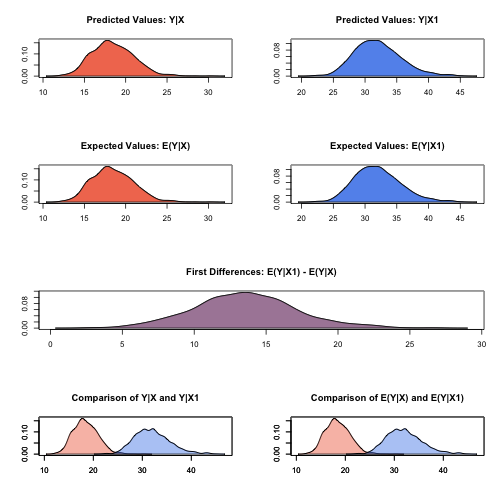
\includegraphics{Zelig-lognorm.png}
\caption{Zelig-lognorm}\end{figure}


\subsection{Model}
\label{vignette:id15}
Let \(Y_i^*\) be the survival time for observation \(i\) with
the density function \(f(y)\) and the corresponding distribution
function \(F(t)=\int_{0}^t f(y) dy\). This variable might be
censored for some observations at a fixed time \(y_c\) such that the
fully observed dependent variable, \(Y_i\), is defined as
\begin{gather}
\begin{split}Y_i = \left\{ \begin{array}{ll}
      Y_i^* & \textrm{if }Y_i^* \leq y_c \\
      y_c & \textrm{if }Y_i^* > y_c \\
    \end{array} \right.\end{split}\notag
\end{gather}\begin{itemize}
\item {} 
The \emph{stochastic component} is described by the distribution of the
partially observed variable, \(Y^*\). For the lognormal model,
there are two equivalent representations:
\begin{gather}
\begin{split}\begin{aligned}
    Y_i^* \; \sim \; \textrm{LogNormal}(\mu_i, \sigma^2) & \textrm{ or
} & \log(Y_i^*) \; \sim \; \textrm{Normal}(\mu_i, \sigma^2)\end{aligned}\end{split}\notag
\end{gather}
where the parameters \(\mu_i\) and \(\sigma^2\) are the mean
and variance of the Normal distribution. (Note that the output from
zelig() parameterizes scale:math:{}` = sigma{}`.)

In addition, survival models like the lognormal have three additional
properties. The hazard function \(h(t)\) measures the probability
of not surviving past time \(t\) given survival up to \(t\).
In general, the hazard function is equal to \(f(t)/S(t)\) where
the survival function \(S(t) =1 - \int_{0}^t f(s) ds\) represents the fraction still surviving at
time \(t\). The cumulative hazard function \(H(t)\) describes
the probability of dying before time \(t\). In general,
\(H(t)=
\int_{0}^{t} h(s) ds = -\log S(t)\). In the case of the lognormal
model,
\begin{gather}
\begin{split}\begin{aligned}
h(t) &=& \frac{1}{\sqrt{2 \pi} \, \sigma t \, S(t)}
\exp\left\{-\frac{1}{2 \sigma^2} (\log \lambda t)^2\right\} \\
S(t) &=& 1 - \Phi\left(\frac{1}{\sigma} \log \lambda t\right) \\
H(t) &=& -\log \left\{ 1 - \Phi\left(\frac{1}{\sigma} \log \lambda t\right) \right\}\end{aligned}\end{split}\notag
\end{gather}
where \(\Phi(\cdot)\) is the cumulative density function for the
Normal distribution.

\item {} 
The \emph{systematic component} is described as:
\begin{gather}
\begin{split}\mu_i = x_i \beta .\end{split}\notag
\end{gather}
\end{itemize}


\subsection{Quantities of Interest}
\label{vignette:id16}\begin{itemize}
\item {} 
The expected values (qi\$ev) for the lognormal model are simulations
of the expected duration:
\begin{gather}
\begin{split}E(Y) =  \exp\left(\mu_i + \frac{1}{2}\sigma^2 \right),\end{split}\notag
\end{gather}
given draws of \(\beta\) and \(\sigma\) from their sampling
distributions.

\item {} 
The predicted value is a draw from the log-normal distribution given
simulations of the parameters \((\lambda_i, \sigma)\).

\item {} 
The first difference (qi\$fd) is
\begin{gather}
\begin{split}\textrm{FD} = E(Y \mid x_1) - E(Y \mid x).\end{split}\notag
\end{gather}
\item {} 
In conditional prediction models, the average expected treatment
effect (att.ev) for the treatment group is
\begin{gather}
\begin{split}\frac{1}{\sum_{i=1}^n t_i}\sum_{i:t_i=1}^n \{ Y_i(t_i=1) - E[Y_i(t_i=0)] \},\end{split}\notag
\end{gather}
where \(t_i\) is a binary explanatory variable defining the
treatment (\(t_i=1\)) and control (\(t_i=0\)) groups. When
\(Y_i(t_i=1)\) is censored rather than observed, we replace it
with a simulation from the model given available knowledge of the
censoring process. Variation in the simulations is due to two
factors: uncertainty in the imputation process for censored
\(y_i^*\) and uncertainty in simulating \(E[Y_i(t_i=0)]\),
the counterfactual expected value of \(Y_i\) for observations in
the treatment group, under the assumption that everything stays the
same except that the treatment indicator is switched to
\(t_i=0\).

\item {} 
In conditional prediction models, the average predicted treatment
effect (att.pr) for the treatment group is
\begin{gather}
\begin{split}\frac{1}{\sum_{i=1}^n t_i} \sum_{i:t_i=1}^n \{  Y_i(t_i=1) -
\widehat{Y_i(t_i=0)} \},\end{split}\notag
\end{gather}
where \(t_i\) is a binary explanatory variable defining the
treatment (\(t_i=1\)) and control (\(t_i=0\)) groups. When
\(Y_i(t_i=1)\) is censored rather than observed, we replace it
with a simulation from the model given available knowledge of the
censoring process. Variation in the simulations are due to two
factors: uncertainty in the imputation process for censored
\(y_i^*\) and uncertainty in simulating
\(\widehat{Y_i(t_i=0)}\), the counterfactual predicted value of
\(Y_i\) for observations in the treatment group, under the
assumption that everything stays the same except that the treatment
indicator is switched to \(t_i=0\).

\end{itemize}


\subsection{Output Values}
\label{vignette:id17}
The output of each Zelig command contains useful information which you
may view. For example, if you run
\code{z.out \textless{}- zelig(Surv(Y, C) \textasciitilde{} X, model = lognorm, data)}, then you may
examine the available information in \code{z.out} by using
\code{names(z.out)}, see the coefficients by using z.out\$coefficients, and
a default summary of information through \code{summary(z.out)}.


\subsection{See also}
\label{vignette:id18}
The exponential function is part of the survival library by by Terry
Therneau, ported to R by Thomas Lumley. Advanced users may wish to refer
to \code{help(survfit)} in the survival library.


\bigskip\hrule{}\bigskip



\section{zelig-ls}
\label{vignette:zelig-ls}
Least Squares Regression for Continuous Dependent Variables

Use least squares regression analysis to estimate the best linear
predictor for the specified dependent variables.


\subsection{Syntax}
\label{vignette:id19}
With reference classes:

\begin{Verbatim}[commandchars=\\\{\}]
z5 \PYG{o}{\PYGZlt{}\PYGZhy{}} zls\PYG{o}{\PYGZdl{}}new\PYG{p}{(}\PYG{p}{)}
z5\PYG{o}{\PYGZdl{}}zelig\PYG{p}{(}Y \PYG{o}{\PYGZti{}} X1 \PYG{o}{+} X \PYG{o}{\PYGZti{}} X\PYG{p}{,} data \PYG{o}{=} mydata\PYG{p}{)}
z5\PYG{o}{\PYGZdl{}}setx\PYG{p}{(}\PYG{p}{)}
z5\PYG{o}{\PYGZdl{}}sim\PYG{p}{(}\PYG{p}{)}
\end{Verbatim}

With the Zelig 4 compatibility wrappers:

\begin{Verbatim}[commandchars=\\\{\}]
z.out \PYG{o}{\PYGZlt{}\PYGZhy{}} zelig\PYG{p}{(}Y \PYG{o}{\PYGZti{}} X1 \PYG{o}{+} X2\PYG{p}{,} model \PYG{o}{=} \PYG{l+s}{\PYGZdq{}}\PYG{l+s}{ls\PYGZdq{}}\PYG{p}{,} data \PYG{o}{=} mydata\PYG{p}{)}
x.out \PYG{o}{\PYGZlt{}\PYGZhy{}} setx\PYG{p}{(}z.out\PYG{p}{)}
s.out \PYG{o}{\PYGZlt{}\PYGZhy{}} sim\PYG{p}{(}z.out\PYG{p}{,} x \PYG{o}{=} x.out\PYG{p}{)}
\end{Verbatim}


\subsection{Examples}
\label{vignette:id20}

\subsubsection{Basic Example with First Differences}
\label{vignette:basic-example-with-first-differences}
Attach sample data:

\begin{Verbatim}[commandchars=\\\{\}]
data\PYG{p}{(}macro\PYG{p}{)}
\end{Verbatim}

Estimate model:

\begin{Verbatim}[commandchars=\\\{\}]
z.out1 \PYG{o}{\PYGZlt{}\PYGZhy{}} zelig\PYG{p}{(}unem \PYG{o}{\PYGZti{}} gdp \PYG{o}{+} capmob \PYG{o}{+} trade\PYG{p}{,} model \PYG{o}{=} \PYG{l+s}{\PYGZdq{}}\PYG{l+s}{ls\PYGZdq{}}\PYG{p}{,} data \PYG{o}{=} macro\PYG{p}{)}
\end{Verbatim}

\begin{Verbatim}[commandchars=\\\{\}]
\PYG{c}{\PYGZsh{}\PYGZsh{} How to cite this model in Zelig:}
\PYG{c}{\PYGZsh{}\PYGZsh{}   Kosuke Imai, Gary King, and Olivia Lau. 2007.}
\PYG{c}{\PYGZsh{}\PYGZsh{}   ls: Least Squares Regression for Continuous Dependent Variables}
\PYG{c}{\PYGZsh{}\PYGZsh{}   in Kosuke Imai, Gary King, and Olivia Lau, \PYGZdq{}Zelig: Everyone\PYGZsq{}s Statistical Software,\PYGZdq{}}
\PYG{c}{\PYGZsh{}\PYGZsh{}   http://datascience.iq.harvard.edu/zelig}
\end{Verbatim}

Summarize regression coefficients:

\begin{Verbatim}[commandchars=\\\{\}]
summary\PYG{p}{(}z.out1\PYG{p}{)}
\end{Verbatim}

\begin{Verbatim}[commandchars=\\\{\}]
\PYG{c}{\PYGZsh{}\PYGZsh{} Model: 1}
\PYG{c}{\PYGZsh{}\PYGZsh{} Call:}
\PYG{c}{\PYGZsh{}\PYGZsh{} stats::lm(formula = unem \PYGZti{} gdp + capmob + trade, data = .)}
\PYG{c}{\PYGZsh{}\PYGZsh{}}
\PYG{c}{\PYGZsh{}\PYGZsh{} Coefficients:}
\PYG{c}{\PYGZsh{}\PYGZsh{} (Intercept)          gdp       capmob        trade}
\PYG{c}{\PYGZsh{}\PYGZsh{}      6.1813      \PYGZhy{}0.3236       1.4219       0.0199}
\PYG{c}{\PYGZsh{}\PYGZsh{}}
\PYG{c}{\PYGZsh{}\PYGZsh{} Next step: Use \PYGZsq{}setx\PYGZsq{} method}
\end{Verbatim}

Set explanatory variables to their default (mean/mode) values, with
high (80th percentile) and low (20th percentile) values for the trade
variable:

\begin{Verbatim}[commandchars=\\\{\}]
x.high \PYG{o}{\PYGZlt{}\PYGZhy{}} setx\PYG{p}{(}z.out1\PYG{p}{,} trade \PYG{o}{=} quantile\PYG{p}{(}macro\PYG{o}{\PYGZdl{}}trade\PYG{p}{,} \PYG{l+m}{0.8}\PYG{p}{)}\PYG{p}{)}
x.low \PYG{o}{\PYGZlt{}\PYGZhy{}} setx\PYG{p}{(}z.out1\PYG{p}{,} trade \PYG{o}{=} quantile\PYG{p}{(}macro\PYG{o}{\PYGZdl{}}trade\PYG{p}{,} \PYG{l+m}{0.2}\PYG{p}{)}\PYG{p}{)}
\end{Verbatim}

Generate first differences for the effect of high versus low trade on GDP:

\begin{Verbatim}[commandchars=\\\{\}]
s.out1 \PYG{o}{\PYGZlt{}\PYGZhy{}} sim\PYG{p}{(}z.out1\PYG{p}{,} x \PYG{o}{=} x.high\PYG{p}{,} x1 \PYG{o}{=} x.low\PYG{p}{)}
\end{Verbatim}

\begin{Verbatim}[commandchars=\\\{\}]
summary\PYG{p}{(}s.out1\PYG{p}{)}
\end{Verbatim}

\begin{Verbatim}[commandchars=\\\{\}]
\PYG{c}{\PYGZsh{}\PYGZsh{}}
\PYG{c}{\PYGZsh{}\PYGZsh{}  sim x :}
\PYG{c}{\PYGZsh{}\PYGZsh{}  \PYGZhy{}\PYGZhy{}\PYGZhy{}\PYGZhy{}\PYGZhy{}}
\PYG{c}{\PYGZsh{}\PYGZsh{} ev}
\PYG{c}{\PYGZsh{}\PYGZsh{}    mean     sd   50\PYGZpc{}  2.5\PYGZpc{} 97.5\PYGZpc{}}
\PYG{c}{\PYGZsh{}\PYGZsh{} 1 5.425 0.1942 5.427 5.017 5.798}
\PYG{c}{\PYGZsh{}\PYGZsh{} pv}
\PYG{c}{\PYGZsh{}\PYGZsh{}    mean     sd   50\PYGZpc{}  2.5\PYGZpc{} 97.5\PYGZpc{}}
\PYG{c}{\PYGZsh{}\PYGZsh{} 1 5.425 0.1942 5.427 5.017 5.798}
\PYG{c}{\PYGZsh{}\PYGZsh{}}
\PYG{c}{\PYGZsh{}\PYGZsh{}  sim x1 :}
\PYG{c}{\PYGZsh{}\PYGZsh{}  \PYGZhy{}\PYGZhy{}\PYGZhy{}\PYGZhy{}\PYGZhy{}}
\PYG{c}{\PYGZsh{}\PYGZsh{} ev}
\PYG{c}{\PYGZsh{}\PYGZsh{}    mean     sd   50\PYGZpc{}  2.5\PYGZpc{} 97.5\PYGZpc{}}
\PYG{c}{\PYGZsh{}\PYGZsh{} 1 4.595 0.1872 4.594 4.241 4.974}
\PYG{c}{\PYGZsh{}\PYGZsh{} pv}
\PYG{c}{\PYGZsh{}\PYGZsh{}    mean     sd   50\PYGZpc{}  2.5\PYGZpc{} 97.5\PYGZpc{}}
\PYG{c}{\PYGZsh{}\PYGZsh{} 1 4.595 0.1872 4.594 4.241 4.974}
\PYG{c}{\PYGZsh{}\PYGZsh{} fd}
\PYG{c}{\PYGZsh{}\PYGZsh{}      mean     sd     50\PYGZpc{}   2.5\PYGZpc{}   97.5\PYGZpc{}}
\PYG{c}{\PYGZsh{}\PYGZsh{} 1 \PYGZhy{}0.8301 0.2399 \PYGZhy{}0.8275 \PYGZhy{}1.321 \PYGZhy{}0.3987}
\end{Verbatim}

\begin{Verbatim}[commandchars=\\\{\}]
plot\PYG{p}{(}s.out1\PYG{p}{)}
\end{Verbatim}
\begin{figure}[htbp]
\centering

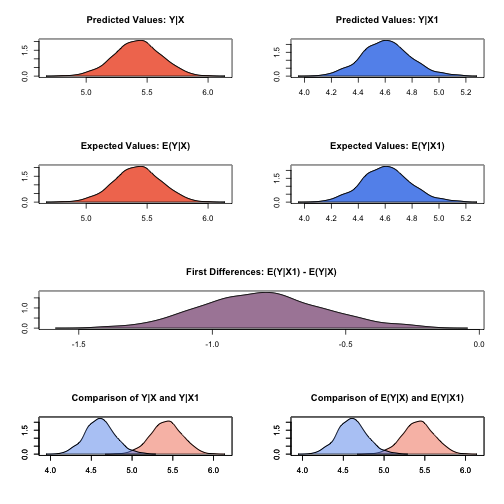
\includegraphics{unnamed-chunk-10.png}
\end{figure}


\subsubsection{Using Dummy Variables}
\label{vignette:using-dummy-variables}
Estimate a model with fixed effects for each country (see for help
with dummy variables). Note that you do not need to create dummy
variables, as the program will automatically parse the unique values
in the selected variable into discrete levels.

\begin{Verbatim}[commandchars=\\\{\}]
z.out2 \PYG{o}{\PYGZlt{}\PYGZhy{}} zelig\PYG{p}{(}unem \PYG{o}{\PYGZti{}} gdp \PYG{o}{+} trade \PYG{o}{+} capmob \PYG{o}{+} as.factor\PYG{p}{(}country\PYG{p}{)}\PYG{p}{,} model \PYG{o}{=} \PYG{l+s}{\PYGZdq{}}\PYG{l+s}{ls\PYGZdq{}}\PYG{p}{,} data \PYG{o}{=} macro\PYG{p}{)}
\end{Verbatim}

\begin{Verbatim}[commandchars=\\\{\}]
\PYG{c}{\PYGZsh{}\PYGZsh{} How to cite this model in Zelig:}
\PYG{c}{\PYGZsh{}\PYGZsh{}   Kosuke Imai, Gary King, and Olivia Lau. 2007.}
\PYG{c}{\PYGZsh{}\PYGZsh{}   ls: Least Squares Regression for Continuous Dependent Variables}
\PYG{c}{\PYGZsh{}\PYGZsh{}   in Kosuke Imai, Gary King, and Olivia Lau, \PYGZdq{}Zelig: Everyone\PYGZsq{}s Statistical Software,\PYGZdq{}}
\PYG{c}{\PYGZsh{}\PYGZsh{}   http://datascience.iq.harvard.edu/zelig}
\end{Verbatim}

Set values for the explanatory variables, using the default mean/mode
values, with country set to the United States and Japan,
respectively:

\begin{Verbatim}[commandchars=\\\{\}]
x.US \PYG{o}{\PYGZlt{}\PYGZhy{}} setx\PYG{p}{(}z.out2\PYG{p}{,} country \PYG{o}{=} \PYG{l+s}{\PYGZdq{}}\PYG{l+s}{United States\PYGZdq{}}\PYG{p}{)}
x.Japan \PYG{o}{\PYGZlt{}\PYGZhy{}} setx\PYG{p}{(}z.out2\PYG{p}{,} country \PYG{o}{=} \PYG{l+s}{\PYGZdq{}}\PYG{l+s}{Japan\PYGZdq{}}\PYG{p}{)}
\end{Verbatim}

Simulate quantities of interest:

\begin{Verbatim}[commandchars=\\\{\}]
s.out2 \PYG{o}{\PYGZlt{}\PYGZhy{}} sim\PYG{p}{(}z.out2\PYG{p}{,} x \PYG{o}{=} x.US\PYG{p}{,} x1 \PYG{o}{=} x.Japan\PYG{p}{)}
\end{Verbatim}

\begin{Verbatim}[commandchars=\\\{\}]
plot\PYG{p}{(}s.out2\PYG{p}{)}
\end{Verbatim}
\begin{figure}[htbp]
\centering

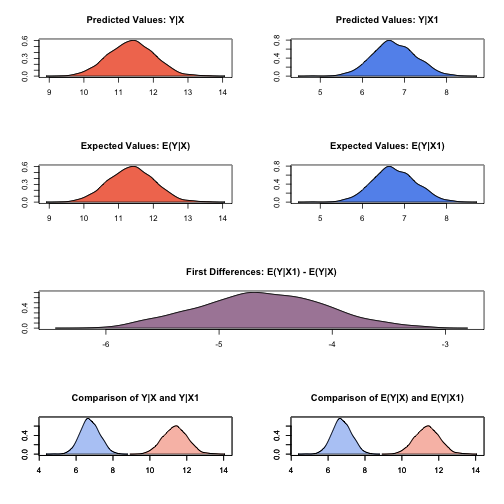
\includegraphics{unnamed-chunk-14.png}
\end{figure}


\subsection{Model}
\label{vignette:id21}\begin{itemize}
\item {} 
The \emph{stochastic component} is described by a density with mean
\(\mu_i\) and the common variance \(\sigma^2\)
\begin{gather}
\begin{split}Y_i \; \sim \; f(y_i \mid \mu_i, \sigma^2).\end{split}\notag
\end{gather}
\item {} 
The \emph{systematic component} models the conditional mean as
\begin{gather}
\begin{split}\mu_i =  x_i \beta\end{split}\notag
\end{gather}
where \(x_i\) is the vector of covariates, and \(\beta\) is
the vector of coefficients.

The least squares estimator is the best linear predictor of a
dependent variable given \(x_i\), and minimizes the sum of
squared residuals, \(\sum_{i=1}^n (Y_i-x_i \beta)^2\).

\end{itemize}


\subsection{Quantities of Interest}
\label{vignette:id22}\begin{itemize}
\item {} 
The expected value (qi\$ev) is the mean of simulations from the
stochastic component,
\begin{gather}
\begin{split}E(Y) = x_i \beta,\end{split}\notag
\end{gather}
given a draw of \(\beta\) from its sampling distribution.

\item {} 
In conditional prediction models, the average expected treatment
effect (att.ev) for the treatment group is
\begin{gather}
\begin{split}\frac{1}{\sum_{i=1}^n t_i}\sum_{i:t_i=1}^n \left\{ Y_i(t_i=1) -
      E[Y_i(t_i=0)] \right\},\end{split}\notag
\end{gather}
where \(t_i\) is a binary explanatory variable defining the
treatment (\(t_i=1\)) and control (\(t_i=0\)) groups.
Variation in the simulations are due to uncertainty in simulating
\(E[Y_i(t_i=0)]\), the counterfactual expected value of
\(Y_i\) for observations in the treatment group, under the
assumption that everything stays the same except that the treatment
indicator is switched to \(t_i=0\).

\end{itemize}


\subsection{Output Values}
\label{vignette:id23}
The output of each Zelig command contains useful information which you
may view. For example, if you run
\code{z.out \textless{}- zelig(y \textasciitilde{} x, model = ls, data)}, then you may examine the
available information in \code{z.out} by using \code{names(z.out)}, see the
coefficients by using z.out\$coefficients, and a default summary of
information through \code{summary(z.out)}. Other elements available through
the \$ operator are listed below.
\begin{itemize}
\item {} 
From the zelig() output object z.out, you may extract:
\begin{itemize}
\item {} 
coefficients: parameter estimates for the explanatory variables.

\item {} 
residuals: the working residuals in the final iteration of the
IWLS fit.

\item {} 
fitted.values: fitted values.

\item {} 
df.residual: the residual degrees of freedom.

\item {} 
zelig.data: the input data frame if save.data = TRUE.

\end{itemize}

\item {} 
From summary(z.out), you may extract:
\begin{itemize}
\item {} 
coefficients: the parameter estimates with their associated
standard errors, \(p\)-values, and \(t\)-statistics.
\begin{gather}
\begin{split}\hat{\beta} \; = \; \left(\sum_{i=1}^n x_i' x_i\right)^{-1} \sum x_i y_i\end{split}\notag
\end{gather}
\item {} 
sigma: the square root of the estimate variance of the random
error \(e\):
\begin{gather}
\begin{split}\hat{\sigma} \; = \; \frac{\sum (Y_i-x_i\hat{\beta})^2}{n-k}\end{split}\notag
\end{gather}
\item {} 
r.squared: the fraction of the variance explained by the model.
\begin{gather}
\begin{split}R^2 \; = \; 1 - \frac{\sum (Y_i-x_i\hat{\beta})^2}{\sum (y_i -
         \bar{y})^2}\end{split}\notag
\end{gather}
\item {} 
adj.r.squared: the above \(R^2\) statistic, penalizing for an
increased number of explanatory variables.

\item {} 
cov.unscaled: a \(k \times k\) matrix of unscaled covariances.

\end{itemize}

\end{itemize}


\subsection{See also}
\label{vignette:id24}
The least squares regression is part of the stats package by William N.
Venables and Brian D. Ripley .In addition, advanced users may wish to
refer to \code{help(lm)} and \code{help(lm.fit)}.


\bigskip\hrule{}\bigskip



\section{zelig-negbin}
\label{vignette:zelig-negbin}
Negative Binomial Regression for Event Count Dependent Variables

Use the negative binomial regression if you have a count of events for
each observation of your dependent variable. The negative binomial model
is frequently used to estimate over-dispersed event count models.


\subsection{Syntax}
\label{vignette:id25}
With reference classes:

\begin{Verbatim}[commandchars=\\\{\}]
z5 \PYG{o}{\PYGZlt{}\PYGZhy{}} znegbin\PYG{o}{\PYGZdl{}}new\PYG{p}{(}\PYG{p}{)}
z5\PYG{o}{\PYGZdl{}}zelig\PYG{p}{(}Y \PYG{o}{\PYGZti{}} X1 \PYG{o}{+} X \PYG{o}{\PYGZti{}} X\PYG{p}{,} data \PYG{o}{=} mydata\PYG{p}{)}
z5\PYG{o}{\PYGZdl{}}setx\PYG{p}{(}\PYG{p}{)}
z5\PYG{o}{\PYGZdl{}}sim\PYG{p}{(}\PYG{p}{)}
\end{Verbatim}

With the Zelig 4 compatibility wrappers:

\begin{Verbatim}[commandchars=\\\{\}]
z.out \PYG{o}{\PYGZlt{}\PYGZhy{}} zelig\PYG{p}{(}Y \PYG{o}{\PYGZti{}} X1 \PYG{o}{+} X2\PYG{p}{,} model \PYG{o}{=} \PYG{l+s}{\PYGZdq{}}\PYG{l+s}{negbin\PYGZdq{}}\PYG{p}{,} data \PYG{o}{=} mydata\PYG{p}{)}
x.out \PYG{o}{\PYGZlt{}\PYGZhy{}} setx\PYG{p}{(}z.out\PYG{p}{)}
s.out \PYG{o}{\PYGZlt{}\PYGZhy{}} sim\PYG{p}{(}z.out\PYG{p}{,} x \PYG{o}{=} x.out\PYG{p}{)}
\end{Verbatim}


\subsection{Example}
\label{vignette:id26}
Load sample data:

\begin{Verbatim}[commandchars=\\\{\}]
data\PYG{p}{(}sanction\PYG{p}{)}
\end{Verbatim}

Estimate the model:

\begin{Verbatim}[commandchars=\\\{\}]
z.out \PYG{o}{\PYGZlt{}\PYGZhy{}} zelig\PYG{p}{(}num \PYG{o}{\PYGZti{}} target \PYG{o}{+} coop\PYG{p}{,} model \PYG{o}{=} \PYG{l+s}{\PYGZdq{}}\PYG{l+s}{negbinom\PYGZdq{}}\PYG{p}{,} data \PYG{o}{=} sanction\PYG{p}{)}
\end{Verbatim}

\begin{Verbatim}[commandchars=\\\{\}]
\PYG{c}{\PYGZsh{}\PYGZsh{} Error: Model \PYGZsq{}negbinom\PYGZsq{} not found}
\end{Verbatim}

\begin{Verbatim}[commandchars=\\\{\}]
summary\PYG{p}{(}z.out\PYG{p}{)}
\end{Verbatim}

\begin{Verbatim}[commandchars=\\\{\}]
\PYG{c}{\PYGZsh{}\PYGZsh{} Model: 1Call:}
\PYG{c}{\PYGZsh{}\PYGZsh{} survival::survreg(formula = Surv(duration, ciep12) \PYGZti{} fract +}
\PYG{c}{\PYGZsh{}\PYGZsh{}     numst2, data = ., dist = \PYGZdq{}lognormal\PYGZdq{}, model = FALSE)}
\PYG{c}{\PYGZsh{}\PYGZsh{}}
\PYG{c}{\PYGZsh{}\PYGZsh{} Coefficients:}
\PYG{c}{\PYGZsh{}\PYGZsh{} (Intercept)       fract      numst2}
\PYG{c}{\PYGZsh{}\PYGZsh{}    5.366670   \PYGZhy{}0.004438    0.559833}
\PYG{c}{\PYGZsh{}\PYGZsh{}}
\PYG{c}{\PYGZsh{}\PYGZsh{} Scale= 1.2}
\PYG{c}{\PYGZsh{}\PYGZsh{}}
\PYG{c}{\PYGZsh{}\PYGZsh{} Loglik(model)= \PYGZhy{}1078   Loglik(intercept only)= \PYGZhy{}1101}
\PYG{c}{\PYGZsh{}\PYGZsh{}  Chisq= 46.58 on 2 degrees of freedom, p= 7.7e\PYGZhy{}11}
\PYG{c}{\PYGZsh{}\PYGZsh{} n= 314}
\PYG{c}{\PYGZsh{}\PYGZsh{} Next step: Use \PYGZsq{}setx\PYGZsq{} method}
\end{Verbatim}

Set values for the explanatory variables to their default mean values:

\begin{Verbatim}[commandchars=\\\{\}]
x.out \PYG{o}{\PYGZlt{}\PYGZhy{}} setx\PYG{p}{(}z.out\PYG{p}{)}
\end{Verbatim}

Simulate fitted values:

\begin{Verbatim}[commandchars=\\\{\}]
s.out \PYG{o}{\PYGZlt{}\PYGZhy{}} sim\PYG{p}{(}z.out\PYG{p}{,} x \PYG{o}{=} x.out\PYG{p}{)}
\end{Verbatim}

\begin{Verbatim}[commandchars=\\\{\}]
summary\PYG{p}{(}s.out\PYG{p}{)}
\end{Verbatim}

\begin{Verbatim}[commandchars=\\\{\}]
\PYG{c}{\PYGZsh{}\PYGZsh{}}
\PYG{c}{\PYGZsh{}\PYGZsh{}  sim x :}
\PYG{c}{\PYGZsh{}\PYGZsh{}  \PYGZhy{}\PYGZhy{}\PYGZhy{}\PYGZhy{}\PYGZhy{}}
\PYG{c}{\PYGZsh{}\PYGZsh{} ev}
\PYG{c}{\PYGZsh{}\PYGZsh{}    mean    sd   50\PYGZpc{}  2.5\PYGZpc{} 97.5\PYGZpc{}}
\PYG{c}{\PYGZsh{}\PYGZsh{} 1 25.94 2.521 25.78 21.25 31.33}
\PYG{c}{\PYGZsh{}\PYGZsh{} pv}
\PYG{c}{\PYGZsh{}\PYGZsh{}    mean    sd   50\PYGZpc{}  2.5\PYGZpc{} 97.5\PYGZpc{}}
\PYG{c}{\PYGZsh{}\PYGZsh{} 1 25.94 2.521 25.78 21.25 31.33}
\end{Verbatim}

\begin{Verbatim}[commandchars=\\\{\}]
plot\PYG{p}{(}s.out\PYG{p}{)}
\end{Verbatim}
\begin{figure}[htbp]
\centering
\capstart

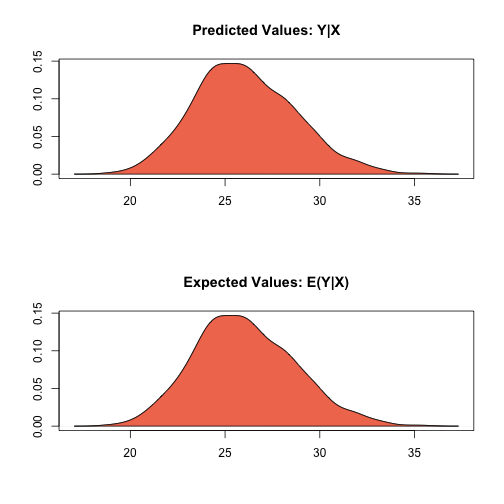
\includegraphics{Zelig-negbin.png}
\caption{Zelig-negbin}\end{figure}


\subsection{Model}
\label{vignette:id27}
Let \(Y_i\) be the number of independent events that occur during a
fixed time period. This variable can take any non-negative integer
value.
\begin{itemize}
\item {} 
The negative binomial distribution is derived by letting the mean of
the Poisson distribution vary according to a fixed parameter
\(\zeta\) given by the Gamma distribution. The \emph{stochastic
component} is given by
\begin{gather}
\begin{split}\begin{aligned}
     Y_i \mid \zeta_i & \sim & \textrm{Poisson}(\zeta_i \mu_i),\\
     \zeta_i & \sim & \frac{1}{\theta}\textrm{Gamma}(\theta).
   \end{aligned}\end{split}\notag
\end{gather}
The marginal distribution of \(Y_i\) is then the negative
binomial with mean \(\mu_i\) and variance
\(\mu_i + \mu_i^2/\theta\):
\begin{gather}
\begin{split}\begin{aligned}
   Y_i & \sim & \textrm{NegBin}(\mu_i, \theta), \\
       & = & \frac{\Gamma (\theta + y_i)}{y! \, \Gamma(\theta)}
             \frac{\mu_i^{y_i} \, \theta^{\theta}}{(\mu_i + \theta)^{\theta + y_i}},
   \end{aligned}\end{split}\notag
\end{gather}
where \(\theta\) is the systematic parameter of the Gamma
distribution modeling \(\zeta_i\).

\item {} 
The \emph{systematic component} is given by
\begin{gather}
\begin{split}\mu_i = \exp(x_i \beta)\end{split}\notag
\end{gather}
where \(x_i\) is the vector of \(k\) explanatory variables
and \(\beta\) is the vector of coefficients.

\end{itemize}


\subsection{Quantities of Interest}
\label{vignette:id28}\begin{itemize}
\item {} 
The expected values (qi\$ev) are simulations of the mean of the
stochastic component. Thus,
\begin{gather}
\begin{split}E(Y) = \mu_i = \exp(x_i
  \beta),\end{split}\notag
\end{gather}
given simulations of \(\beta\).

\item {} 
The predicted value (qi\$pr) drawn from the distribution defined by
the set of parameters \((\mu_i, \theta)\).

\item {} 
The first difference (qi\$fd) is
\begin{gather}
\begin{split}\textrm{FD} \; = \; E(Y | x_1) - E(Y \mid x)\end{split}\notag
\end{gather}
\item {} 
In conditional prediction models, the average expected treatment
effect (att.ev) for the treatment group is
\begin{gather}
\begin{split}\frac{1}{\sum_{i=1}^n t_i}\sum_{i:t_i=1}^n \left\{ Y_i(t_i=1) -
      E[Y_i(t_i=0)] \right\},\end{split}\notag
\end{gather}
where \(t_i\) is a binary explanatory variable defining the
treatment (\(t_i=1\)) and control (\(t_i=0\)) groups.
Variation in the simulations are due to uncertainty in simulating
\(E[Y_i(t_i=0)]\), the counterfactual expected value of
\(Y_i\) for observations in the treatment group, under the
assumption that everything stays the same except that the treatment
indicator is switched to \(t_i=0\).

\item {} 
In conditional prediction models, the average predicted treatment
effect (att.pr) for the treatment group is
\begin{gather}
\begin{split}\frac{1}{\sum_{i=1}^n t_i}\sum_{i:t_i=1}^n \left\{ Y_i(t_i=1) -
      \widehat{Y_i(t_i=0)} \right\},\end{split}\notag
\end{gather}
where \(t_i\) is a binary explanatory variable defining the
treatment (\(t_i=1\)) and control (\(t_i=0\)) groups.
Variation in the simulations are due to uncertainty in simulating
\(\widehat{Y_i(t_i=0)}\), the counterfactual predicted value of
\(Y_i\) for observations in the treatment group, under the
assumption that everything stays the same except that the treatment
indicator is switched to \(t_i=0\).

\end{itemize}


\subsection{Output Values}
\label{vignette:id29}
The output of each Zelig command contains useful information which you
may view. For example, if you run
\code{z.out \textless{}- zelig(y \textasciitilde{} x, model = negbin, data)}, then you may examine
the available information in \code{z.out} by using \code{names(z.out)}, see
the coefficients by using z.out\$coefficients, and a default summary of
information through \code{summary(z.out)}.


\subsection{See also}
\label{vignette:id30}
The negative binomial model is part of the MASS package by William N.
Venable and Brian D. Ripley . Advanced users may wish to refer to
{\color{red}\bfseries{}{}`{}`}help(glm.nb){}`.


\bigskip\hrule{}\bigskip



\section{zelig-normal}
\label{vignette:zelig-normal}
Normal Regression for Continuous Dependent Variables

The Normal regression model is a close variant of the more standard
least squares regression model (see ). Both models specify a continuous
dependent variable as a linear function of a set of explanatory
variables. The Normal model reports maximum likelihood (rather than
least squares) estimates. The two models differ only in their estimate
for the stochastic parameter \(\sigma\).


\subsection{Syntax}
\label{vignette:id33}
With reference classes:

\begin{Verbatim}[commandchars=\\\{\}]
z5 \PYG{o}{\PYGZlt{}\PYGZhy{}} znormal\PYG{o}{\PYGZdl{}}new\PYG{p}{(}\PYG{p}{)}
z5\PYG{o}{\PYGZdl{}}zelig\PYG{p}{(}Y \PYG{o}{\PYGZti{}} X1 \PYG{o}{+} X \PYG{o}{\PYGZti{}} X\PYG{p}{,} data \PYG{o}{=} mydata\PYG{p}{)}
z5\PYG{o}{\PYGZdl{}}setx\PYG{p}{(}\PYG{p}{)}
z5\PYG{o}{\PYGZdl{}}sim\PYG{p}{(}\PYG{p}{)}
\end{Verbatim}

With the Zelig 4 compatibility wrappers:

\begin{Verbatim}[commandchars=\\\{\}]
z.out \PYG{o}{\PYGZlt{}\PYGZhy{}} zelig\PYG{p}{(}Y \PYG{o}{\PYGZti{}} X1 \PYG{o}{+} X2\PYG{p}{,} model \PYG{o}{=} \PYG{l+s}{\PYGZdq{}}\PYG{l+s}{normal\PYGZdq{}}\PYG{p}{,} data \PYG{o}{=} mydata\PYG{p}{)}
x.out \PYG{o}{\PYGZlt{}\PYGZhy{}} setx\PYG{p}{(}z.out\PYG{p}{)}
s.out \PYG{o}{\PYGZlt{}\PYGZhy{}} sim\PYG{p}{(}z.out\PYG{p}{,} x \PYG{o}{=} x.out\PYG{p}{)}
\end{Verbatim}


\subsection{Examples}
\label{vignette:id34}

\subsubsection{Basic Example with First Differences}
\label{vignette:id35}
Attach sample data:

\begin{Verbatim}[commandchars=\\\{\}]
data\PYG{p}{(}macro\PYG{p}{)}
\end{Verbatim}

Estimate model:

\begin{Verbatim}[commandchars=\\\{\}]
z.out1 \PYG{o}{\PYGZlt{}\PYGZhy{}} zelig\PYG{p}{(}unem \PYG{o}{\PYGZti{}} gdp \PYG{o}{+} capmob \PYG{o}{+} trade\PYG{p}{,} model \PYG{o}{=} \PYG{l+s}{\PYGZdq{}}\PYG{l+s}{normal\PYGZdq{}}\PYG{p}{,} data \PYG{o}{=} macro\PYG{p}{)}
\end{Verbatim}

\begin{Verbatim}[commandchars=\\\{\}]
\PYG{c}{\PYGZsh{}\PYGZsh{} How to cite this model in Zelig:}
\PYG{c}{\PYGZsh{}\PYGZsh{}   Kosuke Imai, Gary King, Olivia Lau. 2008.}
\PYG{c}{\PYGZsh{}\PYGZsh{}   normal: Normal Regression for Continuous Dependent Variables}
\PYG{c}{\PYGZsh{}\PYGZsh{}   in Kosuke Imai, Gary King, and Olivia Lau, \PYGZdq{}Zelig: Everyone\PYGZsq{}s Statistical Software,\PYGZdq{}}
\PYG{c}{\PYGZsh{}\PYGZsh{}   http://datascience.iq.harvard.edu/zelig}
\end{Verbatim}

Summarize of regression coefficients:

\begin{Verbatim}[commandchars=\\\{\}]
summary\PYG{p}{(}z.out1\PYG{p}{)}
\end{Verbatim}

\begin{Verbatim}[commandchars=\\\{\}]
\PYG{c}{\PYGZsh{}\PYGZsh{} Model: 1}
\PYG{c}{\PYGZsh{}\PYGZsh{} Call:  stats::glm(formula = unem \PYGZti{} gdp + capmob + trade, family = gaussian(\PYGZdq{}identity\PYGZdq{}),}
\PYG{c}{\PYGZsh{}\PYGZsh{}     data = .)}
\PYG{c}{\PYGZsh{}\PYGZsh{}}
\PYG{c}{\PYGZsh{}\PYGZsh{} Coefficients:}
\PYG{c}{\PYGZsh{}\PYGZsh{} (Intercept)          gdp       capmob        trade}
\PYG{c}{\PYGZsh{}\PYGZsh{}      6.1813      \PYGZhy{}0.3236       1.4219       0.0199}
\PYG{c}{\PYGZsh{}\PYGZsh{}}
\PYG{c}{\PYGZsh{}\PYGZsh{} Degrees of Freedom: 349 Total (i.e. Null);  346 Residual}
\PYG{c}{\PYGZsh{}\PYGZsh{} Null Deviance:       3660}
\PYG{c}{\PYGZsh{}\PYGZsh{} Residual Deviance: 2610  AIC: 1710}
\PYG{c}{\PYGZsh{}\PYGZsh{} Next step: Use \PYGZsq{}setx\PYGZsq{} method}
\end{Verbatim}

Set explanatory variables to their default (mean/mode) values, with
high (80th percentile) and low (20th percentile) values for trade:

\begin{Verbatim}[commandchars=\\\{\}]
x.high \PYG{o}{\PYGZlt{}\PYGZhy{}} setx\PYG{p}{(}z.out1\PYG{p}{,} trade \PYG{o}{=} quantile\PYG{p}{(}macro\PYG{o}{\PYGZdl{}}trade\PYG{p}{,} \PYG{l+m}{0.8}\PYG{p}{)}\PYG{p}{)}
x.low \PYG{o}{\PYGZlt{}\PYGZhy{}} setx\PYG{p}{(}z.out1\PYG{p}{,} trade \PYG{o}{=} quantile\PYG{p}{(}macro\PYG{o}{\PYGZdl{}}trade\PYG{p}{,} \PYG{l+m}{0.2}\PYG{p}{)}\PYG{p}{)}
\end{Verbatim}

Generate first differences for the effect of high versus low trade on GDP:

\begin{Verbatim}[commandchars=\\\{\}]
s.out1 \PYG{o}{\PYGZlt{}\PYGZhy{}} sim\PYG{p}{(}z.out1\PYG{p}{,} x \PYG{o}{=} x.high\PYG{p}{,} x1 \PYG{o}{=} x.low\PYG{p}{)}
\end{Verbatim}

\begin{Verbatim}[commandchars=\\\{\}]
summary\PYG{p}{(}s.out1\PYG{p}{)}
\end{Verbatim}

\begin{Verbatim}[commandchars=\\\{\}]
\PYG{c}{\PYGZsh{}\PYGZsh{}}
\PYG{c}{\PYGZsh{}\PYGZsh{}  sim x :}
\PYG{c}{\PYGZsh{}\PYGZsh{}  \PYGZhy{}\PYGZhy{}\PYGZhy{}\PYGZhy{}\PYGZhy{}}
\PYG{c}{\PYGZsh{}\PYGZsh{} ev}
\PYG{c}{\PYGZsh{}\PYGZsh{}       mean     sd   50\PYGZpc{}  2.5\PYGZpc{} 97.5\PYGZpc{}}
\PYG{c}{\PYGZsh{}\PYGZsh{} [1,] 5.427 0.1956 5.426 5.035 5.804}
\PYG{c}{\PYGZsh{}\PYGZsh{} pv}
\PYG{c}{\PYGZsh{}\PYGZsh{}      mean    sd   50\PYGZpc{}   2.5\PYGZpc{} 97.5\PYGZpc{}}
\PYG{c}{\PYGZsh{}\PYGZsh{} [1,] 5.47 2.676 5.495 0.1705  10.7}
\PYG{c}{\PYGZsh{}\PYGZsh{}}
\PYG{c}{\PYGZsh{}\PYGZsh{}  sim x1 :}
\PYG{c}{\PYGZsh{}\PYGZsh{}  \PYGZhy{}\PYGZhy{}\PYGZhy{}\PYGZhy{}\PYGZhy{}}
\PYG{c}{\PYGZsh{}\PYGZsh{} ev}
\PYG{c}{\PYGZsh{}\PYGZsh{}       mean     sd   50\PYGZpc{}  2.5\PYGZpc{} 97.5\PYGZpc{}}
\PYG{c}{\PYGZsh{}\PYGZsh{} [1,] 4.602 0.1833 4.602 4.235 4.961}
\PYG{c}{\PYGZsh{}\PYGZsh{} pv}
\PYG{c}{\PYGZsh{}\PYGZsh{}       mean    sd  50\PYGZpc{}   2.5\PYGZpc{} 97.5\PYGZpc{}}
\PYG{c}{\PYGZsh{}\PYGZsh{} [1,] 4.637 2.811 4.68 \PYGZhy{}1.085 10.22}
\PYG{c}{\PYGZsh{}\PYGZsh{} fd}
\PYG{c}{\PYGZsh{}\PYGZsh{}         mean     sd     50\PYGZpc{}   2.5\PYGZpc{}   97.5\PYGZpc{}}
\PYG{c}{\PYGZsh{}\PYGZsh{} [1,] \PYGZhy{}0.8257 0.2403 \PYGZhy{}0.8271 \PYGZhy{}1.293 \PYGZhy{}0.3501}
\end{Verbatim}

A visual summary of quantities of interest:

\begin{Verbatim}[commandchars=\\\{\}]
plot\PYG{p}{(}s.out1\PYG{p}{)}
\end{Verbatim}
\begin{figure}[htbp]
\centering
\capstart

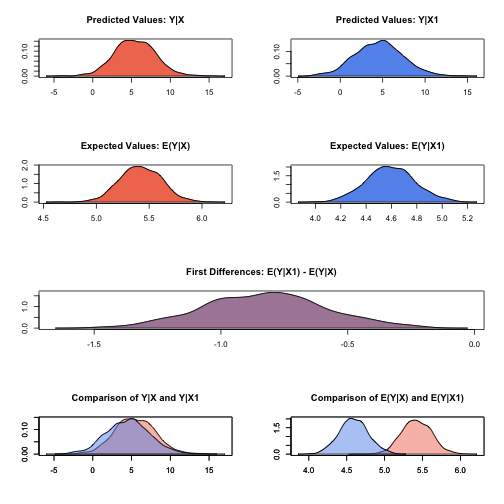
\includegraphics{Zelig-normal.png}
\caption{Zelig-normal}\end{figure}


\subsection{Model}
\label{vignette:id36}
Let \(Y_i\) be the continuous dependent variable for observation
\(i\).
\begin{itemize}
\item {} 
The \emph{stochastic component} is described by a univariate normal model
with a vector of means \(\mu_i\) and scalar variance
\(\sigma^2\):
\begin{gather}
\begin{split}Y_i \; \sim \; \textrm{Normal}(\mu_i, \sigma^2).\end{split}\notag
\end{gather}
\item {} 
The \emph{systematic component} is
\begin{gather}
\begin{split}\mu_i \;= \; x_i \beta,\end{split}\notag
\end{gather}
where \(x_i\) is the vector of \(k\) explanatory variables
and \(\beta\) is the vector of coefficients.

\end{itemize}


\subsection{Quantities of Interest}
\label{vignette:id37}\begin{itemize}
\item {} 
The expected value (qi\$ev) is the mean of simulations from the the
stochastic component,
\begin{gather}
\begin{split}E(Y) = \mu_i = x_i \beta,\end{split}\notag
\end{gather}
given a draw of \(\beta\) from its posterior.

\item {} 
The predicted value (qi\$pr) is drawn from the distribution defined by
the set of parameters \((\mu_i, \sigma)\).

\item {} 
The first difference (qi\$fd) is:
\begin{gather}
\begin{split}\textrm{FD}\; = \;E(Y \mid x_1) -  E(Y \mid x)\end{split}\notag
\end{gather}
\item {} 
In conditional prediction models, the average expected treatment
effect (att.ev) for the treatment group is
\begin{gather}
\begin{split}\frac{1}{\sum_{i=1}^n t_i}\sum_{i:t_i=1}^n \left\{ Y_i(t_i=1) -
      E[Y_i(t_i=0)] \right\},\end{split}\notag
\end{gather}
where \(t_i\) is a binary explanatory variable defining the
treatment (\(t_i=1\)) and control (\(t_i=0\)) groups.
Variation in the simulations are due to uncertainty in simulating
\(E[Y_i(t_i=0)]\), the counterfactual expected value of
\(Y_i\) for observations in the treatment group, under the
assumption that everything stays the same except that the treatment
indicator is switched to \(t_i=0\).

\item {} 
In conditional prediction models, the average predicted treatment
effect (att.pr) for the treatment group is
\begin{gather}
\begin{split}\frac{1}{\sum_{i=1}^n t_i}\sum_{i:t_i=1}^n \left\{ Y_i(t_i=1) -
      \widehat{Y_i(t_i=0)} \right\},\end{split}\notag
\end{gather}
where \(t_i\) is a binary explanatory variable defining the
treatment (\(t_i=1\)) and control (\(t_i=0\)) groups.
Variation in the simulations are due to uncertainty in simulating
\(\widehat{Y_i(t_i=0)}\), the counterfactual predicted value of
\(Y_i\) for observations in the treatment group, under the
assumption that everything stays the same except that the treatment
indicator is switched to \(t_i=0\).

\end{itemize}


\subsection{Output Values}
\label{vignette:id38}
The output of each Zelig command contains useful information which you
may view. For example, if you run
\code{z.out \textless{}- zelig(y \textasciitilde{} x, model = normal, data)}, then you may examine
the available information in \code{z.out} by using \code{names(z.out)}, see
the coefficients by using z.out\$coefficients, and a default summary of
information through \code{summary(z.out)}.


\subsection{See also}
\label{vignette:id39}
The normal model is part of the stats package by . Advanced users may
wish to refer to \code{help(glm)} and \code{help(family)}.


\bigskip\hrule{}\bigskip



\section{zelig-poisson}
\label{vignette:zelig-poisson}
Poisson Regression for Event Count Dependent Variables

Use the Poisson regression model if the observations of your dependent
variable represents the number of independent events that occur during a
fixed period of time (see the negative binomial model, , for
over-dispersed event counts.) For a Bayesian implementation of this
model, see .


\subsection{Syntax}
\label{vignette:id40}
With reference classes:

\begin{Verbatim}[commandchars=\\\{\}]
z5 \PYG{o}{\PYGZlt{}\PYGZhy{}} zpoisson\PYG{o}{\PYGZdl{}}new\PYG{p}{(}\PYG{p}{)}
z5\PYG{o}{\PYGZdl{}}zelig\PYG{p}{(}Y \PYG{o}{\PYGZti{}} X1 \PYG{o}{+} X \PYG{o}{\PYGZti{}} X\PYG{p}{,} data \PYG{o}{=} mydata\PYG{p}{)}
z5\PYG{o}{\PYGZdl{}}setx\PYG{p}{(}\PYG{p}{)}
z5\PYG{o}{\PYGZdl{}}sim\PYG{p}{(}\PYG{p}{)}
\end{Verbatim}

With the Zelig 4 compatibility wrappers:

\begin{Verbatim}[commandchars=\\\{\}]
z.out \PYG{o}{\PYGZlt{}\PYGZhy{}} zelig\PYG{p}{(}Y \PYG{o}{\PYGZti{}} X1 \PYG{o}{+} X2\PYG{p}{,} model \PYG{o}{=} \PYG{l+s}{\PYGZdq{}}\PYG{l+s}{poisson\PYGZdq{}}\PYG{p}{,} data \PYG{o}{=} mydata\PYG{p}{)}
x.out \PYG{o}{\PYGZlt{}\PYGZhy{}} setx\PYG{p}{(}z.out\PYG{p}{)}
s.out \PYG{o}{\PYGZlt{}\PYGZhy{}} sim\PYG{p}{(}z.out\PYG{p}{,} x \PYG{o}{=} x.out\PYG{p}{)}
\end{Verbatim}


\subsection{Example}
\label{vignette:id41}
Load sample data:

\begin{Verbatim}[commandchars=\\\{\}]
data\PYG{p}{(}sanction\PYG{p}{)}
\end{Verbatim}

Estimate Poisson model:

\begin{Verbatim}[commandchars=\\\{\}]
z.out \PYG{o}{\PYGZlt{}\PYGZhy{}} zelig\PYG{p}{(}num \PYG{o}{\PYGZti{}} target \PYG{o}{+} coop\PYG{p}{,} model \PYG{o}{=} \PYG{l+s}{\PYGZdq{}}\PYG{l+s}{poisson\PYGZdq{}}\PYG{p}{,} data \PYG{o}{=} sanction\PYG{p}{)}
\end{Verbatim}

\begin{Verbatim}[commandchars=\\\{\}]
\PYG{c}{\PYGZsh{}\PYGZsh{} How to cite this model in Zelig:}
\PYG{c}{\PYGZsh{}\PYGZsh{}   Kosuke Imai, Gary King, Olivia Lau. 2007.}
\PYG{c}{\PYGZsh{}\PYGZsh{}   poisson: Poisson Regression for Event Count Dependent Variables}
\PYG{c}{\PYGZsh{}\PYGZsh{}   in Kosuke Imai, Gary King, and Olivia Lau, \PYGZdq{}Zelig: Everyone\PYGZsq{}s Statistical Software,\PYGZdq{}}
\PYG{c}{\PYGZsh{}\PYGZsh{}   http://datascience.iq.harvard.edu/zelig}
\end{Verbatim}

\begin{Verbatim}[commandchars=\\\{\}]
summary\PYG{p}{(}z.out\PYG{p}{)}
\end{Verbatim}

\begin{Verbatim}[commandchars=\\\{\}]
\PYG{c}{\PYGZsh{}\PYGZsh{} Model: 1}
\PYG{c}{\PYGZsh{}\PYGZsh{} Call:  stats::glm(formula = num \PYGZti{} target + coop, family = poisson(\PYGZdq{}log\PYGZdq{}),}
\PYG{c}{\PYGZsh{}\PYGZsh{}     data = .)}
\PYG{c}{\PYGZsh{}\PYGZsh{}}
\PYG{c}{\PYGZsh{}\PYGZsh{} Coefficients:}
\PYG{c}{\PYGZsh{}\PYGZsh{} (Intercept)       target         coop}
\PYG{c}{\PYGZsh{}\PYGZsh{}      \PYGZhy{}0.968       \PYGZhy{}0.021        1.211}
\PYG{c}{\PYGZsh{}\PYGZsh{}}
\PYG{c}{\PYGZsh{}\PYGZsh{} Degrees of Freedom: 77 Total (i.e. Null);  75 Residual}
\PYG{c}{\PYGZsh{}\PYGZsh{} Null Deviance:       1580}
\PYG{c}{\PYGZsh{}\PYGZsh{} Residual Deviance: 721   AIC: 944}
\PYG{c}{\PYGZsh{}\PYGZsh{} Next step: Use \PYGZsq{}setx\PYGZsq{} method}
\end{Verbatim}

Set values for the explanatory variables to their default mean values:

\begin{Verbatim}[commandchars=\\\{\}]
x.out \PYG{o}{\PYGZlt{}\PYGZhy{}} setx\PYG{p}{(}z.out\PYG{p}{)}
\end{Verbatim}

Simulate fitted values:

\begin{Verbatim}[commandchars=\\\{\}]
s.out \PYG{o}{\PYGZlt{}\PYGZhy{}} sim\PYG{p}{(}z.out\PYG{p}{,} x \PYG{o}{=} x.out\PYG{p}{)}
summary\PYG{p}{(}s.out\PYG{p}{)}
\end{Verbatim}

\begin{Verbatim}[commandchars=\\\{\}]
\PYG{c}{\PYGZsh{}\PYGZsh{}}
\PYG{c}{\PYGZsh{}\PYGZsh{}  sim x :}
\PYG{c}{\PYGZsh{}\PYGZsh{}  \PYGZhy{}\PYGZhy{}\PYGZhy{}\PYGZhy{}\PYGZhy{}}
\PYG{c}{\PYGZsh{}\PYGZsh{} ev}
\PYG{c}{\PYGZsh{}\PYGZsh{}      mean     sd   50\PYGZpc{} 2.5\PYGZpc{} 97.5\PYGZpc{}}
\PYG{c}{\PYGZsh{}\PYGZsh{} [1,] 3.25 0.2333 3.247 2.82 3.758}
\PYG{c}{\PYGZsh{}\PYGZsh{} pv}
\PYG{c}{\PYGZsh{}\PYGZsh{}       mean    sd 50\PYGZpc{} 2.5\PYGZpc{} 97.5\PYGZpc{}}
\PYG{c}{\PYGZsh{}\PYGZsh{} [1,] 3.259 1.843   3    0     7}
\end{Verbatim}

\begin{Verbatim}[commandchars=\\\{\}]
plot\PYG{p}{(}s.out\PYG{p}{)}
\end{Verbatim}
\begin{figure}[htbp]
\centering
\capstart

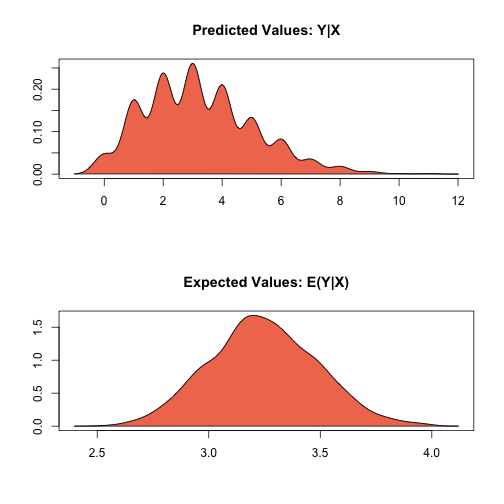
\includegraphics{Zelig-poisson.png}
\caption{Zelig-poisson}\end{figure}


\subsection{Model}
\label{vignette:id42}
Let \(Y_i\) be the number of independent events that occur during a
fixed time period. This variable can take any non-negative integer.
\begin{itemize}
\item {} 
The Poisson distribution has \emph{stochastic component}
\begin{gather}
\begin{split}Y_i \; \sim \; \textrm{Poisson}(\lambda_i),\end{split}\notag
\end{gather}
where \(\lambda_i\) is the mean and variance parameter.

\item {} 
The \emph{systematic component} is
\begin{gather}
\begin{split}\lambda_i \; = \; \exp(x_i \beta),\end{split}\notag
\end{gather}
where \(x_i\) is the vector of explanatory variables, and
\(\beta\) is the vector of coefficients.

\end{itemize}


\subsection{Quantities of Interest}
\label{vignette:id43}\begin{itemize}
\item {} 
The expected value (qi\$ev) is the mean of simulations from the
stochastic component,
\begin{gather}
\begin{split}E(Y) = \lambda_i =  \exp(x_i
  \beta),\end{split}\notag
\end{gather}
given draws of \(\beta\) from its sampling distribution.

\item {} 
The predicted value (qi\$pr) is a random draw from the poisson
distribution defined by mean \(\lambda_i\).

\item {} 
The first difference in the expected values (qi\$fd) is given by:
\begin{gather}
\begin{split}\textrm{FD} \; = \; E(Y | x_1) - E(Y \mid x)\end{split}\notag
\end{gather}
\item {} 
In conditional prediction models, the average expected treatment
effect (att.ev) for the treatment group is
\begin{gather}
\begin{split}\frac{1}{\sum_{i=1}^n t_i}\sum_{i:t_i=1}^n \left\{ Y_i(t_i=1) -
      E[Y_i(t_i=0)] \right\},\end{split}\notag
\end{gather}
where \(t_i\) is a binary explanatory variable defining the
treatment (\(t_i=1\)) and control (\(t_i=0\)) groups.
Variation in the simulations are due to uncertainty in simulating
\(E[Y_i(t_i=0)]\), the counterfactual expected value of
\(Y_i\) for observations in the treatment group, under the
assumption that everything stays the same except that the treatment
indicator is switched to \(t_i=0\).

\item {} 
In conditional prediction models, the average predicted treatment
effect (att.pr) for the treatment group is
\begin{gather}
\begin{split}\frac{1}{\sum_{i=1}^n t_i}\sum_{i:t_i=1}^n \left\{ Y_i(t_i=1) -
      \widehat{Y_i(t_i=0)} \right\},\end{split}\notag
\end{gather}
where \(t_i\) is a binary explanatory variable defining the
treatment (\(t_i=1\)) and control (\(t_i=0\)) groups.
Variation in the simulations are due to uncertainty in simulating
\(\widehat{Y_i(t_i=0)}\), the counterfactual predicted value of
\(Y_i\) for observations in the treatment group, under the
assumption that everything stays the same except that the treatment
indicator is switched to \(t_i=0\).

\end{itemize}


\subsection{Output Values}
\label{vignette:id44}
The output of each Zelig command contains useful information which you
may view. For example, if you run
\code{z.out \textless{}- zelig(y \textasciitilde{} x, model = poisson, data)}, then you may examine
the available information in \code{z.out} by using \code{names(z.out)}, see
the coefficients by using z.out\$coefficients, and a default summary of
information through \code{summary(z.out)}.


\subsection{See also}
\label{vignette:id45}
The poisson model is part of the stats package by . Advanced users may
wish to refer to \code{help(glm)} and \code{help(family)}.


\bigskip\hrule{}\bigskip



\section{zelig-probit}
\label{vignette:zelig-probit}
Probit Regression for Dichotomous Dependent Variables

Use probit regression to model binary dependent variables specified as a
function of a set of explanatory variables.


\subsection{Syntax}
\label{vignette:id46}
With reference classes:

\begin{Verbatim}[commandchars=\\\{\}]
z5 \PYG{o}{\PYGZlt{}\PYGZhy{}} zprobit\PYG{o}{\PYGZdl{}}new\PYG{p}{(}\PYG{p}{)}
z5\PYG{o}{\PYGZdl{}}zelig\PYG{p}{(}Y \PYG{o}{\PYGZti{}} X1 \PYG{o}{+} X \PYG{o}{\PYGZti{}} X\PYG{p}{,} data \PYG{o}{=} mydata\PYG{p}{)}
z5\PYG{o}{\PYGZdl{}}setx\PYG{p}{(}\PYG{p}{)}
z5\PYG{o}{\PYGZdl{}}sim\PYG{p}{(}\PYG{p}{)}
\end{Verbatim}

With the Zelig 4 compatibility wrappers:

\begin{Verbatim}[commandchars=\\\{\}]
z.out \PYG{o}{\PYGZlt{}\PYGZhy{}} zelig\PYG{p}{(}Y \PYG{o}{\PYGZti{}} X1 \PYG{o}{+} X2\PYG{p}{,} model \PYG{o}{=} \PYG{l+s}{\PYGZdq{}}\PYG{l+s}{probit\PYGZdq{}}\PYG{p}{,} data \PYG{o}{=} mydata\PYG{p}{)}
x.out \PYG{o}{\PYGZlt{}\PYGZhy{}} setx\PYG{p}{(}z.out\PYG{p}{)}
s.out \PYG{o}{\PYGZlt{}\PYGZhy{}} sim\PYG{p}{(}z.out\PYG{p}{,} x \PYG{o}{=} x.out\PYG{p}{,} x1 \PYG{o}{=} \PYG{k+kc}{NULL}\PYG{p}{)}
\end{Verbatim}


\subsection{Example}
\label{vignette:id47}
Attach the sample turnout dataset:

\begin{Verbatim}[commandchars=\\\{\}]
data\PYG{p}{(}turnout\PYG{p}{)}
\end{Verbatim}

Estimate parameter values for the probit regression:

\begin{Verbatim}[commandchars=\\\{\}]
z.out \PYG{o}{\PYGZlt{}\PYGZhy{}} zelig\PYG{p}{(}vote \PYG{o}{\PYGZti{}} race \PYG{o}{+} educate\PYG{p}{,} model \PYG{o}{=} \PYG{l+s}{\PYGZdq{}}\PYG{l+s}{probit\PYGZdq{}}\PYG{p}{,} data \PYG{o}{=} turnout\PYG{p}{)}
\end{Verbatim}

\begin{Verbatim}[commandchars=\\\{\}]
\PYG{c}{\PYGZsh{}\PYGZsh{} How to cite this model in Zelig:}
\PYG{c}{\PYGZsh{}\PYGZsh{}   Kosuke Imai, Gary King, Olivia Lau. 2007.}
\PYG{c}{\PYGZsh{}\PYGZsh{}   probit: Probit Regression for Dichotomous Dependent Variables}
\PYG{c}{\PYGZsh{}\PYGZsh{}   in Kosuke Imai, Gary King, and Olivia Lau, \PYGZdq{}Zelig: Everyone\PYGZsq{}s Statistical Software,\PYGZdq{}}
\PYG{c}{\PYGZsh{}\PYGZsh{}   http://datascience.iq.harvard.edu/zelig}
\end{Verbatim}

\begin{Verbatim}[commandchars=\\\{\}]
summary\PYG{p}{(}z.out\PYG{p}{)}
\end{Verbatim}

\begin{Verbatim}[commandchars=\\\{\}]
\PYG{c}{\PYGZsh{}\PYGZsh{} Model: 1}
\PYG{c}{\PYGZsh{}\PYGZsh{} Call:  stats::glm(formula = vote \PYGZti{} race + educate, family = binomial(\PYGZdq{}probit\PYGZdq{}),}
\PYG{c}{\PYGZsh{}\PYGZsh{}     data = .)}
\PYG{c}{\PYGZsh{}\PYGZsh{}}
\PYG{c}{\PYGZsh{}\PYGZsh{} Coefficients:}
\PYG{c}{\PYGZsh{}\PYGZsh{} (Intercept)    racewhite      educate}
\PYG{c}{\PYGZsh{}\PYGZsh{}     \PYGZhy{}0.7259       0.2991       0.0971}
\PYG{c}{\PYGZsh{}\PYGZsh{}}
\PYG{c}{\PYGZsh{}\PYGZsh{} Degrees of Freedom: 1999 Total (i.e. Null);  1997 Residual}
\PYG{c}{\PYGZsh{}\PYGZsh{} Null Deviance:       2270}
\PYG{c}{\PYGZsh{}\PYGZsh{} Residual Deviance: 2140  AIC: 2140}
\PYG{c}{\PYGZsh{}\PYGZsh{} Next step: Use \PYGZsq{}setx\PYGZsq{} method}
\end{Verbatim}

Set values for the explanatory variables to their default values.

\begin{Verbatim}[commandchars=\\\{\}]
x.out \PYG{o}{\PYGZlt{}\PYGZhy{}} setx\PYG{p}{(}z.out\PYG{p}{)}
\end{Verbatim}

Simulate quantities of interest from the posterior distribution.

\begin{Verbatim}[commandchars=\\\{\}]
s.out \PYG{o}{\PYGZlt{}\PYGZhy{}} sim\PYG{p}{(}z.out\PYG{p}{,} x \PYG{o}{=} x.out\PYG{p}{)}
\end{Verbatim}

\begin{Verbatim}[commandchars=\\\{\}]
summary\PYG{p}{(}s.out\PYG{p}{)}
\end{Verbatim}

\begin{Verbatim}[commandchars=\\\{\}]
plot\PYG{p}{(}s.out1\PYG{p}{)}
\end{Verbatim}
\begin{figure}[htbp]
\centering
\capstart

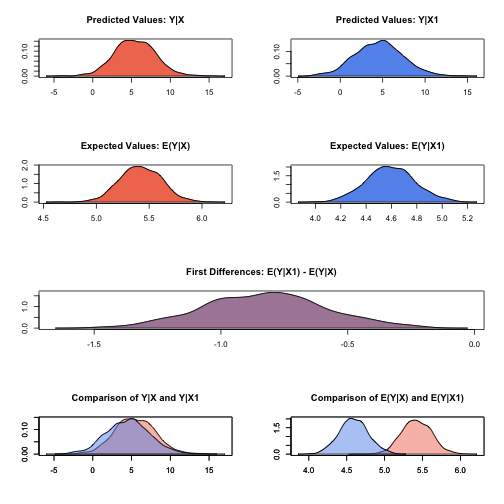
\includegraphics{Zelig-probit.png}
\caption{Zelig-probi}\end{figure}


\subsection{Model}
\label{vignette:id48}
Let \(Y_i\) be the observed binary dependent variable for
observation \(i\) which takes the value of either 0 or 1.
\begin{itemize}
\item {} 
The \emph{stochastic component} is given by
\begin{gather}
\begin{split}Y_i \; \sim \; \textrm{Bernoulli}(\pi_i),\end{split}\notag
\end{gather}
where \(\pi_i=\Pr(Y_i=1)\).

\item {} 
The \emph{systematic component} is
\begin{gather}
\begin{split}\pi_i \; = \; \Phi (x_i \beta)\end{split}\notag
\end{gather}
where \(\Phi(\mu)\) is the cumulative distribution function of
the Normal distribution with mean 0 and unit variance.

\end{itemize}


\subsection{Quantities of Interest}
\label{vignette:id49}\begin{itemize}
\item {} 
The expected value (qi\$ev) is a simulation of predicted probability
of success
\begin{gather}
\begin{split}E(Y) = \pi_i = \Phi(x_i
  \beta),\end{split}\notag
\end{gather}
given a draw of \(\beta\) from its sampling distribution.

\item {} 
The predicted value (qi\$pr) is a draw from a Bernoulli distribution
with mean \(\pi_i\).

\item {} 
The first difference (qi\$fd) in expected values is defined as
\begin{gather}
\begin{split}\textrm{FD} = \Pr(Y = 1 \mid x_1) - \Pr(Y = 1 \mid x).\end{split}\notag
\end{gather}
\item {} 
The risk ratio (qi\$rr) is defined as
\begin{gather}
\begin{split}\textrm{RR} = \Pr(Y = 1 \mid x_1) / \Pr(Y = 1 \mid x).\end{split}\notag
\end{gather}
\item {} 
In conditional prediction models, the average expected treatment
effect (att.ev) for the treatment group is
\begin{gather}
\begin{split}\frac{1}{\sum_{i=1}^n t_i}\sum_{i:t_i=1}^n \left\{ Y_i(t_i=1) -
      E[Y_i(t_i=0)] \right\},\end{split}\notag
\end{gather}
where \(t_i\) is a binary explanatory variable defining the
treatment (\(t_i=1\)) and control (\(t_i=0\)) groups.
Variation in the simulations are due to uncertainty in simulating
\(E[Y_i(t_i=0)]\), the counterfactual expected value of
\(Y_i\) for observations in the treatment group, under the
assumption that everything stays the same except that the treatment
indicator is switched to \(t_i=0\).

\item {} 
In conditional prediction models, the average predicted treatment
effect (att.pr) for the treatment group is
\begin{gather}
\begin{split}\frac{1}{\sum_{i=1}^n t_i}\sum_{i:t_i=1}^n \left\{ Y_i(t_i=1) -
      \widehat{Y_i(t_i=0)} \right\},\end{split}\notag
\end{gather}
where \(t_i\) is a binary explanatory variable defining the
treatment (\(t_i=1\)) and control (\(t_i=0\)) groups.
Variation in the simulations are due to uncertainty in simulating
\(\widehat{Y_i(t_i=0)}\), the counterfactual predicted value of
\(Y_i\) for observations in the treatment group, under the
assumption that everything stays the same except that the treatment
indicator is switched to \(t_i=0\).

\end{itemize}


\subsection{Output Values}
\label{vignette:id50}
The output of each Zelig command contains useful information which you
may view. For example, if you run
\code{z.out \textless{}- zelig(y \textasciitilde{} x, model = probit, data)}, then you may examine
the available information in \code{z.out} by using \code{names(z.out)}, see
the coefficients by using z.out\$coefficients, and a default summary of
information through \code{summary(z.out)}.


\subsection{See also}
\label{vignette:id51}
The probit model is part of the stats package by . Advanced users may
wish to refer to \code{help(glm)} and \code{help(family)}.


\bigskip\hrule{}\bigskip



\section{zelig-relogit}
\label{vignette:zelig-relogit}
Rare Events Logistic Regression for Dichotomous Dependent Variables

The relogit procedure estimates the same model as standard logistic
regression (appropriate when you have a dichotomous dependent variable
and a set of explanatory variables; see ), but the estimates are
corrected for the bias that occurs when the sample is small or the
observed events are rare (i.e., if the dependent variable has many more
1s than 0s or the reverse). The relogit procedure also optionally uses
prior correction for case-control sampling designs.


\subsection{Syntax}
\label{vignette:id52}
With reference classes:

\begin{Verbatim}[commandchars=\\\{\}]
z5 \PYG{o}{\PYGZlt{}\PYGZhy{}} zrelogit\PYG{o}{\PYGZdl{}}new\PYG{p}{(}\PYG{p}{)}
z5\PYG{o}{\PYGZdl{}}zelig\PYG{p}{(}Y \PYG{o}{\PYGZti{}} X1 \PYG{o}{+} X2\PYG{p}{,} tau \PYG{o}{=} \PYG{k+kc}{NULL}\PYG{p}{,}
                       case.control \PYG{o}{=} c\PYG{p}{(}\PYG{l+s}{\PYGZdq{}}\PYG{l+s}{prior\PYGZdq{}}\PYG{p}{,} \PYG{l+s}{\PYGZdq{}}\PYG{l+s}{weighting\PYGZdq{}}\PYG{p}{)}\PYG{p}{,}
                       bias.correct \PYG{o}{=} \PYG{k+kc}{TRUE}\PYG{p}{,} robust \PYG{o}{=} \PYG{k+kc}{FALSE}\PYG{p}{,}
                       data \PYG{o}{=} mydata\PYG{p}{,} \PYG{k+kc}{...}\PYG{p}{)}
z5\PYG{o}{\PYGZdl{}}setx\PYG{p}{(}\PYG{p}{)}
z5\PYG{o}{\PYGZdl{}}sim\PYG{p}{(}\PYG{p}{)}
\end{Verbatim}

With the Zelig 4 compatibility wrappers:

\begin{Verbatim}[commandchars=\\\{\}]
z.out \PYG{o}{\PYGZlt{}\PYGZhy{}} zelig\PYG{p}{(}Y \PYG{o}{\PYGZti{}} X1 \PYG{o}{+} X2\PYG{p}{,} model \PYG{o}{=} \PYG{l+s}{\PYGZdq{}}\PYG{l+s}{relogit\PYGZdq{}}\PYG{p}{,} tau \PYG{o}{=} \PYG{k+kc}{NULL}\PYG{p}{,}
                       case.control \PYG{o}{=} c\PYG{p}{(}\PYG{l+s}{\PYGZdq{}}\PYG{l+s}{prior\PYGZdq{}}\PYG{p}{,} \PYG{l+s}{\PYGZdq{}}\PYG{l+s}{weighting\PYGZdq{}}\PYG{p}{)}\PYG{p}{,}
                       bias.correct \PYG{o}{=} \PYG{k+kc}{TRUE}\PYG{p}{,} robust \PYG{o}{=} \PYG{k+kc}{FALSE}\PYG{p}{,}
                       data \PYG{o}{=} mydata\PYG{p}{,} \PYG{k+kc}{...}\PYG{p}{)}
x.out \PYG{o}{\PYGZlt{}\PYGZhy{}} setx\PYG{p}{(}z.out\PYG{p}{)}
s.out \PYG{o}{\PYGZlt{}\PYGZhy{}} sim\PYG{p}{(}z.out\PYG{p}{,} x \PYG{o}{=} x.out\PYG{p}{)}
\end{Verbatim}


\subsection{Arguments}
\label{vignette:arguments}
The relogit procedure supports four optional arguments in addition to
the standard arguments for zelig(). You may additionally use:
\begin{itemize}
\item {} 
tau: a vector containing either one or two values for \(\tau\),
the true population fraction of ones. Use, for example, tau = c(0.05,
0.1) to specify that the lower bound on tau is 0.05 and the upper
bound is 0.1. If left unspecified, only finite-sample bias correction
is performed, not case-control correction.

\item {} 
case.control: if tau is specified, choose a method to correct for
case-control sampling design: “prior” (default) or “weighting”.

\item {} 
bias.correct: a logical value of TRUE (default) or FALSE indicating
whether the intercept should be corrected for finite sample (rare
events) bias.

\end{itemize}

Note that if tau = NULL, bias.correct = FALSE, the
relogit procedure performs a standard logistic regression without any
correction.


\subsection{Example 1: One Tau with Prior Correction and Bias Correction}
\label{vignette:example-1-one-tau-with-prior-correction-and-bias-correction}
Due to memory and space considerations, the data used here are a sample
drawn from the full data set used in King and Zeng, 2001, The proportion
of militarized interstate conflicts to the absence of disputes is
\(\tau = 1,042 / 303,772
\approx 0.00343\). To estimate the model,

\begin{Verbatim}[commandchars=\\\{\}]
data\PYG{p}{(}mid\PYG{p}{)}
\end{Verbatim}

\begin{Verbatim}[commandchars=\\\{\}]
z.out1 \PYG{o}{\PYGZlt{}\PYGZhy{}} zelig\PYG{p}{(}conflict \PYG{o}{\PYGZti{}} major \PYG{o}{+} contig \PYG{o}{+} power \PYG{o}{+} maxdem \PYG{o}{+} mindem \PYG{o}{+} years\PYG{p}{,} data \PYG{o}{=} mid\PYG{p}{,} model \PYG{o}{=} \PYG{l+s}{\PYGZdq{}}\PYG{l+s}{relogit\PYGZdq{}}\PYG{p}{,} tau \PYG{o}{=} \PYG{l+m}{1042}\PYG{o}{/}\PYG{l+m}{303772}\PYG{p}{)}
\end{Verbatim}

\begin{Verbatim}[commandchars=\\\{\}]
\PYG{c}{\PYGZsh{}\PYGZsh{} How to cite this model in Zelig:}
\PYG{c}{\PYGZsh{}\PYGZsh{}   Kosuke Imai, Gary King, and Olivia Lau. 2014.}
\PYG{c}{\PYGZsh{}\PYGZsh{}   relogit: Rare Events Logistic Regression for Dichotomous Dependent Variables}
\PYG{c}{\PYGZsh{}\PYGZsh{}   in Kosuke Imai, Gary King, and Olivia Lau, \PYGZdq{}Zelig: Everyone\PYGZsq{}s Statistical Software,\PYGZdq{}}
\PYG{c}{\PYGZsh{}\PYGZsh{}   http://datascience.iq.harvard.edu/zelig}
\end{Verbatim}

Summarize the model output:

\begin{Verbatim}[commandchars=\\\{\}]
summary\PYG{p}{(}z.out1\PYG{p}{)}
\end{Verbatim}

\begin{Verbatim}[commandchars=\\\{\}]
\PYG{c}{\PYGZsh{}\PYGZsh{} Model: 1}
\PYG{c}{\PYGZsh{}\PYGZsh{} Call:  relogit(formula = cbind(conflict, 1 \PYGZhy{} conflict) \PYGZti{} major + contig +}
\PYG{c}{\PYGZsh{}\PYGZsh{}     power + maxdem + mindem + years, data = ., tau = 0.00343020423212146,}
\PYG{c}{\PYGZsh{}\PYGZsh{}     bias.correct = TRUE, case.control = \PYGZdq{}prior\PYGZdq{})}
\PYG{c}{\PYGZsh{}\PYGZsh{}}
\PYG{c}{\PYGZsh{}\PYGZsh{} Coefficients:}
\PYG{c}{\PYGZsh{}\PYGZsh{} (Intercept)        major       contig        power       maxdem}
\PYG{c}{\PYGZsh{}\PYGZsh{}     \PYGZhy{}7.5084       2.4320       4.1080       1.0536       0.0480}
\PYG{c}{\PYGZsh{}\PYGZsh{}      mindem        years}
\PYG{c}{\PYGZsh{}\PYGZsh{}     \PYGZhy{}0.0641      \PYGZhy{}0.0629}
\PYG{c}{\PYGZsh{}\PYGZsh{}}
\PYG{c}{\PYGZsh{}\PYGZsh{} Degrees of Freedom: 3125 Total (i.e. Null);  3119 Residual}
\PYG{c}{\PYGZsh{}\PYGZsh{} Null Deviance:       3980}
\PYG{c}{\PYGZsh{}\PYGZsh{} Residual Deviance: 1870  AIC: 1880}
\PYG{c}{\PYGZsh{}\PYGZsh{} Next step: Use \PYGZsq{}setx\PYGZsq{} method}
\end{Verbatim}

Set the explanatory variables to their means:

\begin{Verbatim}[commandchars=\\\{\}]
x.out1 \PYG{o}{\PYGZlt{}\PYGZhy{}} setx\PYG{p}{(}z.out1\PYG{p}{)}
\end{Verbatim}

Simulate quantities of interest:

\begin{Verbatim}[commandchars=\\\{\}]
s.out1 \PYG{o}{\PYGZlt{}\PYGZhy{}} sim\PYG{p}{(}z.out1\PYG{p}{,} x \PYG{o}{=} x.out1\PYG{p}{)}
summary\PYG{p}{(}s.out1\PYG{p}{)}
\end{Verbatim}

\begin{Verbatim}[commandchars=\\\{\}]
\PYG{c}{\PYGZsh{}\PYGZsh{}}
\PYG{c}{\PYGZsh{}\PYGZsh{}  sim x :}
\PYG{c}{\PYGZsh{}\PYGZsh{}  \PYGZhy{}\PYGZhy{}\PYGZhy{}\PYGZhy{}\PYGZhy{}}
\PYG{c}{\PYGZsh{}\PYGZsh{} ev}
\PYG{c}{\PYGZsh{}\PYGZsh{}          mean        sd      50\PYGZpc{}     2.5\PYGZpc{}    97.5\PYGZpc{}}
\PYG{c}{\PYGZsh{}\PYGZsh{} [1,] 0.002398 0.0001509 0.002394 0.002116 0.002693}
\PYG{c}{\PYGZsh{}\PYGZsh{} pv}
\PYG{c}{\PYGZsh{}\PYGZsh{}          0     1}
\PYG{c}{\PYGZsh{}\PYGZsh{} [1,] 0.997 0.003}
\end{Verbatim}

\begin{Verbatim}[commandchars=\\\{\}]
plot\PYG{p}{(}s.out1\PYG{p}{)}
\end{Verbatim}
\begin{figure}[htbp]
\centering
\capstart


\includegraphics{Zelig-relogit.png}
\caption{Zelig-relogit}\end{figure}


\subsection{Example 2: One Tau with Weighting, Robust Standard Errors, and Bias Correction}
\label{vignette:example-2-one-tau-with-weighting-robust-standard-errors-and-bias-correction}
Suppose that we wish to perform case control correction using weighting
(rather than the default prior correction). To estimate the model:

\begin{Verbatim}[commandchars=\\\{\}]
z.out2 \PYG{o}{\PYGZlt{}\PYGZhy{}} zelig\PYG{p}{(}conflict \PYG{o}{\PYGZti{}} major \PYG{o}{+} contig \PYG{o}{+} power \PYG{o}{+} maxdem \PYG{o}{+} mindem \PYG{o}{+} years\PYG{p}{,} data \PYG{o}{=} mid\PYG{p}{,} model \PYG{o}{=} \PYG{l+s}{\PYGZdq{}}\PYG{l+s}{relogit\PYGZdq{}}\PYG{p}{,} tau \PYG{o}{=} \PYG{l+m}{1042}\PYG{o}{/}\PYG{l+m}{303772}\PYG{p}{,} case.control \PYG{o}{=} \PYG{l+s}{\PYGZdq{}}\PYG{l+s}{weighting\PYGZdq{}}\PYG{p}{,} robust \PYG{o}{=} \PYG{k+kc}{TRUE}\PYG{p}{)}
\end{Verbatim}

\begin{Verbatim}[commandchars=\\\{\}]
\PYG{c}{\PYGZsh{}\PYGZsh{} Error: unused argument (robust = TRUE)}
\end{Verbatim}

Summarize the model output:

\begin{Verbatim}[commandchars=\\\{\}]
summary\PYG{p}{(}z.out2\PYG{p}{)}
\end{Verbatim}

\begin{Verbatim}[commandchars=\\\{\}]
\PYG{c}{\PYGZsh{}\PYGZsh{} Model: 1}
\PYG{c}{\PYGZsh{}\PYGZsh{} Call:}
\PYG{c}{\PYGZsh{}\PYGZsh{} stats::lm(formula = unem \PYGZti{} gdp + trade + capmob + as.factor(country),}
\PYG{c}{\PYGZsh{}\PYGZsh{}     data = .)}
\PYG{c}{\PYGZsh{}\PYGZsh{}}
\PYG{c}{\PYGZsh{}\PYGZsh{} Coefficients:}
\PYG{c}{\PYGZsh{}\PYGZsh{}                      (Intercept)                               gdp}
\PYG{c}{\PYGZsh{}\PYGZsh{}                           \PYGZhy{}5.843                            \PYGZhy{}0.110}
\PYG{c}{\PYGZsh{}\PYGZsh{}                            trade                            capmob}
\PYG{c}{\PYGZsh{}\PYGZsh{}                            0.144                             0.815}
\PYG{c}{\PYGZsh{}\PYGZsh{}        as.factor(country)Belgium          as.factor(country)Canada}
\PYG{c}{\PYGZsh{}\PYGZsh{}                           \PYGZhy{}1.599                             6.759}
\PYG{c}{\PYGZsh{}\PYGZsh{}        as.factor(country)Denmark         as.factor(country)Finland}
\PYG{c}{\PYGZsh{}\PYGZsh{}                            4.311                             4.810}
\PYG{c}{\PYGZsh{}\PYGZsh{}         as.factor(country)France           as.factor(country)Italy}
\PYG{c}{\PYGZsh{}\PYGZsh{}                            6.905                             9.290}
\PYG{c}{\PYGZsh{}\PYGZsh{}          as.factor(country)Japan     as.factor(country)Netherlands}
\PYG{c}{\PYGZsh{}\PYGZsh{}                            5.459                            \PYGZhy{}1.459}
\PYG{c}{\PYGZsh{}\PYGZsh{}         as.factor(country)Norway          as.factor(country)Sweden}
\PYG{c}{\PYGZsh{}\PYGZsh{}                           \PYGZhy{}2.754                             0.925}
\PYG{c}{\PYGZsh{}\PYGZsh{} as.factor(country)United Kingdom   as.factor(country)United States}
\PYG{c}{\PYGZsh{}\PYGZsh{}                            5.601                            10.066}
\PYG{c}{\PYGZsh{}\PYGZsh{}   as.factor(country)West Germany}
\PYG{c}{\PYGZsh{}\PYGZsh{}                            3.364}
\PYG{c}{\PYGZsh{}\PYGZsh{}}
\PYG{c}{\PYGZsh{}\PYGZsh{} Next step: Use \PYGZsq{}setx\PYGZsq{} method}
\end{Verbatim}

Set the explanatory variables to their means:

\begin{Verbatim}[commandchars=\\\{\}]
x.out2 \PYG{o}{\PYGZlt{}\PYGZhy{}} setx\PYG{p}{(}z.out2\PYG{p}{)}
\end{Verbatim}

Simulate quantities of interest:

\begin{Verbatim}[commandchars=\\\{\}]
s.out2 \PYG{o}{\PYGZlt{}\PYGZhy{}} sim\PYG{p}{(}z.out2\PYG{p}{,} x \PYG{o}{=} x.out2\PYG{p}{)}
summary\PYG{p}{(}s.out2\PYG{p}{)}
\end{Verbatim}

\begin{Verbatim}[commandchars=\\\{\}]
\PYG{c}{\PYGZsh{}\PYGZsh{}}
\PYG{c}{\PYGZsh{}\PYGZsh{}  sim x :}
\PYG{c}{\PYGZsh{}\PYGZsh{}  \PYGZhy{}\PYGZhy{}\PYGZhy{}\PYGZhy{}\PYGZhy{}}
\PYG{c}{\PYGZsh{}\PYGZsh{} ev}
\PYG{c}{\PYGZsh{}\PYGZsh{}    mean     sd   50\PYGZpc{}  2.5\PYGZpc{} 97.5\PYGZpc{}}
\PYG{c}{\PYGZsh{}\PYGZsh{} 1 8.049 0.4152 8.041 7.259 8.841}
\PYG{c}{\PYGZsh{}\PYGZsh{} pv}
\PYG{c}{\PYGZsh{}\PYGZsh{}    mean     sd   50\PYGZpc{}  2.5\PYGZpc{} 97.5\PYGZpc{}}
\PYG{c}{\PYGZsh{}\PYGZsh{} 1 8.049 0.4152 8.041 7.259 8.841}
\end{Verbatim}


\subsection{Example 3: Two Taus with Bias Correction and Prior Correction}
\label{vignette:example-3-two-taus-with-bias-correction-and-prior-correction}
Suppose that we did not know that \(\tau \approx 0.00343\), but only
that it was somewhere between \((0.002, 0.005)\). To estimate a
model with a range of feasible estimates for \(\tau\) (using the
default prior correction method for case control correction):

\begin{Verbatim}[commandchars=\\\{\}]
z.out2 \PYG{o}{\PYGZlt{}\PYGZhy{}} zelig\PYG{p}{(}conflict \PYG{o}{\PYGZti{}} major \PYG{o}{+} contig \PYG{o}{+} power \PYG{o}{+} maxdem \PYG{o}{+} mindem \PYG{o}{+} years\PYG{p}{,} data \PYG{o}{=} mid\PYG{p}{,} model \PYG{o}{=} \PYG{l+s}{\PYGZdq{}}\PYG{l+s}{relogit\PYGZdq{}}\PYG{p}{,} tau \PYG{o}{=} c\PYG{p}{(}\PYG{l+m}{0.002}\PYG{p}{,} \PYG{l+m}{0.005}\PYG{p}{)}\PYG{p}{)}
\end{Verbatim}

\begin{Verbatim}[commandchars=\\\{\}]
\PYG{c}{\PYGZsh{}\PYGZsh{} How to cite this model in Zelig:}
\PYG{c}{\PYGZsh{}\PYGZsh{}   Kosuke Imai, Gary King, and Olivia Lau. 2014.}
\PYG{c}{\PYGZsh{}\PYGZsh{}   relogit: Rare Events Logistic Regression for Dichotomous Dependent Variables}
\PYG{c}{\PYGZsh{}\PYGZsh{}   in Kosuke Imai, Gary King, and Olivia Lau, \PYGZdq{}Zelig: Everyone\PYGZsq{}s Statistical Software,\PYGZdq{}}
\PYG{c}{\PYGZsh{}\PYGZsh{}   http://datascience.iq.harvard.edu/zelig}
\end{Verbatim}

Summarize the model output:

\begin{Verbatim}[commandchars=\\\{\}]
z.out2
\end{Verbatim}

\begin{Verbatim}[commandchars=\\\{\}]
\PYG{c}{\PYGZsh{}\PYGZsh{} Model: 1\PYGZdl{}lower.estimate}
\PYG{c}{\PYGZsh{}\PYGZsh{}}
\PYG{c}{\PYGZsh{}\PYGZsh{} Call:  (function (formula, data = sys.parent(), tau = NULL, bias.correct = TRUE,}
\PYG{c}{\PYGZsh{}\PYGZsh{}     case.control = \PYGZdq{}prior\PYGZdq{}, ...)}
\PYG{c}{\PYGZsh{}\PYGZsh{} \PYGZob{}}
\PYG{c}{\PYGZsh{}\PYGZsh{}     mf \PYGZlt{}\PYGZhy{} match.call()}
\PYG{c}{\PYGZsh{}\PYGZsh{}     mf\PYGZdl{}tau \PYGZlt{}\PYGZhy{} mf\PYGZdl{}bias.correct \PYGZlt{}\PYGZhy{} mf\PYGZdl{}case.control \PYGZlt{}\PYGZhy{} NULL}
\PYG{c}{\PYGZsh{}\PYGZsh{}     if (!is.null(tau)) \PYGZob{}}
\PYG{c}{\PYGZsh{}\PYGZsh{}         tau \PYGZlt{}\PYGZhy{} unique(tau)}
\PYG{c}{\PYGZsh{}\PYGZsh{}         if (length(case.control) \PYGZgt{} 1)}
\PYG{c}{\PYGZsh{}\PYGZsh{}             stop(\PYGZdq{}You can only choose one option for case control correction.\PYGZdq{})}
\PYG{c}{\PYGZsh{}\PYGZsh{}         ck1 \PYGZlt{}\PYGZhy{} grep(\PYGZdq{}p\PYGZdq{}, case.control)}
\PYG{c}{\PYGZsh{}\PYGZsh{}         ck2 \PYGZlt{}\PYGZhy{} grep(\PYGZdq{}w\PYGZdq{}, case.control)}
\PYG{c}{\PYGZsh{}\PYGZsh{}         if (length(ck1) == 0 \PYGZam{} length(ck2) == 0)}
\PYG{c}{\PYGZsh{}\PYGZsh{}             stop(\PYGZdq{}choose either case.control = \PYGZbs{}\PYGZdq{}prior\PYGZbs{}\PYGZdq{} \PYGZdq{}, \PYGZdq{}or case.control = \PYGZbs{}\PYGZdq{}weighting\PYGZbs{}\PYGZdq{}\PYGZdq{})}
\PYG{c}{\PYGZsh{}\PYGZsh{}         if (length(ck2) == 0)}
\PYG{c}{\PYGZsh{}\PYGZsh{}             weighting \PYGZlt{}\PYGZhy{} FALSE}
\PYG{c}{\PYGZsh{}\PYGZsh{}         else weighting \PYGZlt{}\PYGZhy{} TRUE}
\PYG{c}{\PYGZsh{}\PYGZsh{}     \PYGZcb{}}
\PYG{c}{\PYGZsh{}\PYGZsh{}     else weighting \PYGZlt{}\PYGZhy{} FALSE}
\PYG{c}{\PYGZsh{}\PYGZsh{}     if (length(tau) \PYGZgt{} 2)}
\PYG{c}{\PYGZsh{}\PYGZsh{}         stop(\PYGZdq{}tau must be a vector of length less than or equal to 2\PYGZdq{})}
\PYG{c}{\PYGZsh{}\PYGZsh{}     else if (length(tau) == 2) \PYGZob{}}
\PYG{c}{\PYGZsh{}\PYGZsh{}         mf[[1]] \PYGZlt{}\PYGZhy{} relogit}
\PYG{c}{\PYGZsh{}\PYGZsh{}         res \PYGZlt{}\PYGZhy{} list()}
\PYG{c}{\PYGZsh{}\PYGZsh{}         mf\PYGZdl{}tau \PYGZlt{}\PYGZhy{} min(tau)}
\PYG{c}{\PYGZsh{}\PYGZsh{}         res\PYGZdl{}lower.estimate \PYGZlt{}\PYGZhy{} eval(as.call(mf), parent.frame())}
\PYG{c}{\PYGZsh{}\PYGZsh{}         mf\PYGZdl{}tau \PYGZlt{}\PYGZhy{} max(tau)}
\PYG{c}{\PYGZsh{}\PYGZsh{}         res\PYGZdl{}upper.estimate \PYGZlt{}\PYGZhy{} eval(as.call(mf), parent.frame())}
\PYG{c}{\PYGZsh{}\PYGZsh{}         res\PYGZdl{}formula \PYGZlt{}\PYGZhy{} formula}
\PYG{c}{\PYGZsh{}\PYGZsh{}         class(res) \PYGZlt{}\PYGZhy{} c(\PYGZdq{}Relogit2\PYGZdq{}, \PYGZdq{}Relogit\PYGZdq{})}
\PYG{c}{\PYGZsh{}\PYGZsh{}         return(res)}
\PYG{c}{\PYGZsh{}\PYGZsh{}     \PYGZcb{}}
\PYG{c}{\PYGZsh{}\PYGZsh{}     else \PYGZob{}}
\PYG{c}{\PYGZsh{}\PYGZsh{}         mf[[1]] \PYGZlt{}\PYGZhy{} glm}
\PYG{c}{\PYGZsh{}\PYGZsh{}         mf\PYGZdl{}family \PYGZlt{}\PYGZhy{} binomial(link = \PYGZdq{}logit\PYGZdq{})}
\PYG{c}{\PYGZsh{}\PYGZsh{}         y2 \PYGZlt{}\PYGZhy{} model.response(model.frame(mf\PYGZdl{}formula, data))}
\PYG{c}{\PYGZsh{}\PYGZsh{}         if (is.matrix(y2))}
\PYG{c}{\PYGZsh{}\PYGZsh{}             y \PYGZlt{}\PYGZhy{} y2[, 1]}
\PYG{c}{\PYGZsh{}\PYGZsh{}         else y \PYGZlt{}\PYGZhy{} y2}
\PYG{c}{\PYGZsh{}\PYGZsh{}         ybar \PYGZlt{}\PYGZhy{} mean(y)}
\PYG{c}{\PYGZsh{}\PYGZsh{}         if (weighting) \PYGZob{}}
\PYG{c}{\PYGZsh{}\PYGZsh{}             w1 \PYGZlt{}\PYGZhy{} tau/ybar}
\PYG{c}{\PYGZsh{}\PYGZsh{}             w0 \PYGZlt{}\PYGZhy{} (1 \PYGZhy{} tau)/(1 \PYGZhy{} ybar)}
\PYG{c}{\PYGZsh{}\PYGZsh{}             wi \PYGZlt{}\PYGZhy{} w1 * y + w0 * (1 \PYGZhy{} y)}
\PYG{c}{\PYGZsh{}\PYGZsh{}             mf\PYGZdl{}weights \PYGZlt{}\PYGZhy{} wi}
\PYG{c}{\PYGZsh{}\PYGZsh{}         \PYGZcb{}}
\PYG{c}{\PYGZsh{}\PYGZsh{}         res \PYGZlt{}\PYGZhy{} eval(as.call(mf), parent.frame())}
\PYG{c}{\PYGZsh{}\PYGZsh{}         res\PYGZdl{}call \PYGZlt{}\PYGZhy{} match.call(expand.dots = TRUE)}
\PYG{c}{\PYGZsh{}\PYGZsh{}         res\PYGZdl{}tau \PYGZlt{}\PYGZhy{} tau}
\PYG{c}{\PYGZsh{}\PYGZsh{}         X \PYGZlt{}\PYGZhy{} model.matrix(res)}
\PYG{c}{\PYGZsh{}\PYGZsh{}         if (bias.correct) \PYGZob{}}
\PYG{c}{\PYGZsh{}\PYGZsh{}             pihat \PYGZlt{}\PYGZhy{} fitted(res)}
\PYG{c}{\PYGZsh{}\PYGZsh{}             if (is.null(tau))}
\PYG{c}{\PYGZsh{}\PYGZsh{}                 wi \PYGZlt{}\PYGZhy{} rep(1, length(y))}
\PYG{c}{\PYGZsh{}\PYGZsh{}             else if (weighting)}
\PYG{c}{\PYGZsh{}\PYGZsh{}                 res\PYGZdl{}weighting \PYGZlt{}\PYGZhy{} TRUE}
\PYG{c}{\PYGZsh{}\PYGZsh{}             else \PYGZob{}}
\PYG{c}{\PYGZsh{}\PYGZsh{}                 w1 \PYGZlt{}\PYGZhy{} tau/ybar}
\PYG{c}{\PYGZsh{}\PYGZsh{}                 w0 \PYGZlt{}\PYGZhy{} (1 \PYGZhy{} tau)/(1 \PYGZhy{} ybar)}
\PYG{c}{\PYGZsh{}\PYGZsh{}                 wi \PYGZlt{}\PYGZhy{} w1 * y + w0 * (1 \PYGZhy{} y)}
\PYG{c}{\PYGZsh{}\PYGZsh{}                 res\PYGZdl{}weighting \PYGZlt{}\PYGZhy{} FALSE}
\PYG{c}{\PYGZsh{}\PYGZsh{}             \PYGZcb{}}
\PYG{c}{\PYGZsh{}\PYGZsh{}             W \PYGZlt{}\PYGZhy{} pihat * (1 \PYGZhy{} pihat) * wi}
\PYG{c}{\PYGZsh{}\PYGZsh{}             Qdiag \PYGZlt{}\PYGZhy{} lm.influence(lm(y \PYGZti{} X \PYGZhy{} 1, weights = W))\PYGZdl{}hat/W}
\PYG{c}{\PYGZsh{}\PYGZsh{}             if (is.null(tau))}
\PYG{c}{\PYGZsh{}\PYGZsh{}                 xi \PYGZlt{}\PYGZhy{} 0.5 * Qdiag * (2 * pihat \PYGZhy{} 1)}
\PYG{c}{\PYGZsh{}\PYGZsh{}             else xi \PYGZlt{}\PYGZhy{} 0.5 * Qdiag * ((1 + w0) * pihat \PYGZhy{} w0)}
\PYG{c}{\PYGZsh{}\PYGZsh{}             res\PYGZdl{}coefficients \PYGZlt{}\PYGZhy{} res\PYGZdl{}coefficients \PYGZhy{} lm(xi \PYGZti{} X \PYGZhy{}}
\PYG{c}{\PYGZsh{}\PYGZsh{}                 1, weights = W)\PYGZdl{}coefficients}
\PYG{c}{\PYGZsh{}\PYGZsh{}             res\PYGZdl{}bias.correct \PYGZlt{}\PYGZhy{} TRUE}
\PYG{c}{\PYGZsh{}\PYGZsh{}         \PYGZcb{}}
\PYG{c}{\PYGZsh{}\PYGZsh{}         else res\PYGZdl{}bias.correct \PYGZlt{}\PYGZhy{} FALSE}
\PYG{c}{\PYGZsh{}\PYGZsh{}         if (!is.null(tau) \PYGZam{} !weighting) \PYGZob{}}
\PYG{c}{\PYGZsh{}\PYGZsh{}             if (tau \PYGZlt{}= 0 \textbar{}\textbar{} tau \PYGZgt{}= 1)}
\PYG{c}{\PYGZsh{}\PYGZsh{}                 stop(\PYGZdq{}\PYGZbs{}ntau needs to be between 0 and 1.\PYGZbs{}n\PYGZdq{})}
\PYG{c}{\PYGZsh{}\PYGZsh{}             res\PYGZdl{}coefficients[\PYGZdq{}(Intercept)\PYGZdq{}] \PYGZlt{}\PYGZhy{} res\PYGZdl{}coefficients[\PYGZdq{}(Intercept)\PYGZdq{}] \PYGZhy{}}
\PYG{c}{\PYGZsh{}\PYGZsh{}                 log(((1 \PYGZhy{} tau)/tau) * (ybar/(1 \PYGZhy{} ybar)))}
\PYG{c}{\PYGZsh{}\PYGZsh{}             res\PYGZdl{}prior.correct \PYGZlt{}\PYGZhy{} TRUE}
\PYG{c}{\PYGZsh{}\PYGZsh{}             res\PYGZdl{}weighting \PYGZlt{}\PYGZhy{} FALSE}
\PYG{c}{\PYGZsh{}\PYGZsh{}         \PYGZcb{}}
\PYG{c}{\PYGZsh{}\PYGZsh{}         else res\PYGZdl{}prior.correct \PYGZlt{}\PYGZhy{} FALSE}
\PYG{c}{\PYGZsh{}\PYGZsh{}         if (is.null(res\PYGZdl{}weighting))}
\PYG{c}{\PYGZsh{}\PYGZsh{}             res\PYGZdl{}weighting \PYGZlt{}\PYGZhy{} FALSE}
\PYG{c}{\PYGZsh{}\PYGZsh{}         res\PYGZdl{}linear.predictors \PYGZlt{}\PYGZhy{} t(res\PYGZdl{}coefficients) \PYGZpc{}*\PYGZpc{} t(X)}
\PYG{c}{\PYGZsh{}\PYGZsh{}         res\PYGZdl{}fitted.values \PYGZlt{}\PYGZhy{} 1/(1 + exp(\PYGZhy{}res\PYGZdl{}linear.predictors))}
\PYG{c}{\PYGZsh{}\PYGZsh{}         res\PYGZdl{}zelig \PYGZlt{}\PYGZhy{} \PYGZdq{}Relogit\PYGZdq{}}
\PYG{c}{\PYGZsh{}\PYGZsh{}         class(res) \PYGZlt{}\PYGZhy{} c(\PYGZdq{}Relogit\PYGZdq{}, \PYGZdq{}glm\PYGZdq{})}
\PYG{c}{\PYGZsh{}\PYGZsh{}         return(res)}
\PYG{c}{\PYGZsh{}\PYGZsh{}     \PYGZcb{}}
\PYG{c}{\PYGZsh{}\PYGZsh{} \PYGZcb{})(formula = cbind(conflict, 1 \PYGZhy{} conflict) \PYGZti{} major + contig +}
\PYG{c}{\PYGZsh{}\PYGZsh{}     power + maxdem + mindem + years, data = ., tau = 0.002)}
\PYG{c}{\PYGZsh{}\PYGZsh{}}
\PYG{c}{\PYGZsh{}\PYGZsh{} Coefficients:}
\PYG{c}{\PYGZsh{}\PYGZsh{} (Intercept)        major       contig        power       maxdem}
\PYG{c}{\PYGZsh{}\PYGZsh{}     \PYGZhy{}8.0492       2.4320       4.1079       1.0536       0.0480}
\PYG{c}{\PYGZsh{}\PYGZsh{}      mindem        years}
\PYG{c}{\PYGZsh{}\PYGZsh{}     \PYGZhy{}0.0641      \PYGZhy{}0.0629}
\PYG{c}{\PYGZsh{}\PYGZsh{}}
\PYG{c}{\PYGZsh{}\PYGZsh{} Degrees of Freedom: 3125 Total (i.e. Null);  3119 Residual}
\PYG{c}{\PYGZsh{}\PYGZsh{} Null Deviance:       3980}
\PYG{c}{\PYGZsh{}\PYGZsh{} Residual Deviance: 1870  AIC: 1880}
\PYG{c}{\PYGZsh{}\PYGZsh{}}
\PYG{c}{\PYGZsh{}\PYGZsh{} \PYGZdl{}upper.estimate}
\PYG{c}{\PYGZsh{}\PYGZsh{}}
\PYG{c}{\PYGZsh{}\PYGZsh{} Call:  (function (formula, data = sys.parent(), tau = NULL, bias.correct = TRUE,}
\PYG{c}{\PYGZsh{}\PYGZsh{}     case.control = \PYGZdq{}prior\PYGZdq{}, ...)}
\PYG{c}{\PYGZsh{}\PYGZsh{} \PYGZob{}}
\PYG{c}{\PYGZsh{}\PYGZsh{}     mf \PYGZlt{}\PYGZhy{} match.call()}
\PYG{c}{\PYGZsh{}\PYGZsh{}     mf\PYGZdl{}tau \PYGZlt{}\PYGZhy{} mf\PYGZdl{}bias.correct \PYGZlt{}\PYGZhy{} mf\PYGZdl{}case.control \PYGZlt{}\PYGZhy{} NULL}
\PYG{c}{\PYGZsh{}\PYGZsh{}     if (!is.null(tau)) \PYGZob{}}
\PYG{c}{\PYGZsh{}\PYGZsh{}         tau \PYGZlt{}\PYGZhy{} unique(tau)}
\PYG{c}{\PYGZsh{}\PYGZsh{}         if (length(case.control) \PYGZgt{} 1)}
\PYG{c}{\PYGZsh{}\PYGZsh{}             stop(\PYGZdq{}You can only choose one option for case control correction.\PYGZdq{})}
\PYG{c}{\PYGZsh{}\PYGZsh{}         ck1 \PYGZlt{}\PYGZhy{} grep(\PYGZdq{}p\PYGZdq{}, case.control)}
\PYG{c}{\PYGZsh{}\PYGZsh{}         ck2 \PYGZlt{}\PYGZhy{} grep(\PYGZdq{}w\PYGZdq{}, case.control)}
\PYG{c}{\PYGZsh{}\PYGZsh{}         if (length(ck1) == 0 \PYGZam{} length(ck2) == 0)}
\PYG{c}{\PYGZsh{}\PYGZsh{}             stop(\PYGZdq{}choose either case.control = \PYGZbs{}\PYGZdq{}prior\PYGZbs{}\PYGZdq{} \PYGZdq{}, \PYGZdq{}or case.control = \PYGZbs{}\PYGZdq{}weighting\PYGZbs{}\PYGZdq{}\PYGZdq{})}
\PYG{c}{\PYGZsh{}\PYGZsh{}         if (length(ck2) == 0)}
\PYG{c}{\PYGZsh{}\PYGZsh{}             weighting \PYGZlt{}\PYGZhy{} FALSE}
\PYG{c}{\PYGZsh{}\PYGZsh{}         else weighting \PYGZlt{}\PYGZhy{} TRUE}
\PYG{c}{\PYGZsh{}\PYGZsh{}     \PYGZcb{}}
\PYG{c}{\PYGZsh{}\PYGZsh{}     else weighting \PYGZlt{}\PYGZhy{} FALSE}
\PYG{c}{\PYGZsh{}\PYGZsh{}     if (length(tau) \PYGZgt{} 2)}
\PYG{c}{\PYGZsh{}\PYGZsh{}         stop(\PYGZdq{}tau must be a vector of length less than or equal to 2\PYGZdq{})}
\PYG{c}{\PYGZsh{}\PYGZsh{}     else if (length(tau) == 2) \PYGZob{}}
\PYG{c}{\PYGZsh{}\PYGZsh{}         mf[[1]] \PYGZlt{}\PYGZhy{} relogit}
\PYG{c}{\PYGZsh{}\PYGZsh{}         res \PYGZlt{}\PYGZhy{} list()}
\PYG{c}{\PYGZsh{}\PYGZsh{}         mf\PYGZdl{}tau \PYGZlt{}\PYGZhy{} min(tau)}
\PYG{c}{\PYGZsh{}\PYGZsh{}         res\PYGZdl{}lower.estimate \PYGZlt{}\PYGZhy{} eval(as.call(mf), parent.frame())}
\PYG{c}{\PYGZsh{}\PYGZsh{}         mf\PYGZdl{}tau \PYGZlt{}\PYGZhy{} max(tau)}
\PYG{c}{\PYGZsh{}\PYGZsh{}         res\PYGZdl{}upper.estimate \PYGZlt{}\PYGZhy{} eval(as.call(mf), parent.frame())}
\PYG{c}{\PYGZsh{}\PYGZsh{}         res\PYGZdl{}formula \PYGZlt{}\PYGZhy{} formula}
\PYG{c}{\PYGZsh{}\PYGZsh{}         class(res) \PYGZlt{}\PYGZhy{} c(\PYGZdq{}Relogit2\PYGZdq{}, \PYGZdq{}Relogit\PYGZdq{})}
\PYG{c}{\PYGZsh{}\PYGZsh{}         return(res)}
\PYG{c}{\PYGZsh{}\PYGZsh{}     \PYGZcb{}}
\PYG{c}{\PYGZsh{}\PYGZsh{}     else \PYGZob{}}
\PYG{c}{\PYGZsh{}\PYGZsh{}         mf[[1]] \PYGZlt{}\PYGZhy{} glm}
\PYG{c}{\PYGZsh{}\PYGZsh{}         mf\PYGZdl{}family \PYGZlt{}\PYGZhy{} binomial(link = \PYGZdq{}logit\PYGZdq{})}
\PYG{c}{\PYGZsh{}\PYGZsh{}         y2 \PYGZlt{}\PYGZhy{} model.response(model.frame(mf\PYGZdl{}formula, data))}
\PYG{c}{\PYGZsh{}\PYGZsh{}         if (is.matrix(y2))}
\PYG{c}{\PYGZsh{}\PYGZsh{}             y \PYGZlt{}\PYGZhy{} y2[, 1]}
\PYG{c}{\PYGZsh{}\PYGZsh{}         else y \PYGZlt{}\PYGZhy{} y2}
\PYG{c}{\PYGZsh{}\PYGZsh{}         ybar \PYGZlt{}\PYGZhy{} mean(y)}
\PYG{c}{\PYGZsh{}\PYGZsh{}         if (weighting) \PYGZob{}}
\PYG{c}{\PYGZsh{}\PYGZsh{}             w1 \PYGZlt{}\PYGZhy{} tau/ybar}
\PYG{c}{\PYGZsh{}\PYGZsh{}             w0 \PYGZlt{}\PYGZhy{} (1 \PYGZhy{} tau)/(1 \PYGZhy{} ybar)}
\PYG{c}{\PYGZsh{}\PYGZsh{}             wi \PYGZlt{}\PYGZhy{} w1 * y + w0 * (1 \PYGZhy{} y)}
\PYG{c}{\PYGZsh{}\PYGZsh{}             mf\PYGZdl{}weights \PYGZlt{}\PYGZhy{} wi}
\PYG{c}{\PYGZsh{}\PYGZsh{}         \PYGZcb{}}
\PYG{c}{\PYGZsh{}\PYGZsh{}         res \PYGZlt{}\PYGZhy{} eval(as.call(mf), parent.frame())}
\PYG{c}{\PYGZsh{}\PYGZsh{}         res\PYGZdl{}call \PYGZlt{}\PYGZhy{} match.call(expand.dots = TRUE)}
\PYG{c}{\PYGZsh{}\PYGZsh{}         res\PYGZdl{}tau \PYGZlt{}\PYGZhy{} tau}
\PYG{c}{\PYGZsh{}\PYGZsh{}         X \PYGZlt{}\PYGZhy{} model.matrix(res)}
\PYG{c}{\PYGZsh{}\PYGZsh{}         if (bias.correct) \PYGZob{}}
\PYG{c}{\PYGZsh{}\PYGZsh{}             pihat \PYGZlt{}\PYGZhy{} fitted(res)}
\PYG{c}{\PYGZsh{}\PYGZsh{}             if (is.null(tau))}
\PYG{c}{\PYGZsh{}\PYGZsh{}                 wi \PYGZlt{}\PYGZhy{} rep(1, length(y))}
\PYG{c}{\PYGZsh{}\PYGZsh{}             else if (weighting)}
\PYG{c}{\PYGZsh{}\PYGZsh{}                 res\PYGZdl{}weighting \PYGZlt{}\PYGZhy{} TRUE}
\PYG{c}{\PYGZsh{}\PYGZsh{}             else \PYGZob{}}
\PYG{c}{\PYGZsh{}\PYGZsh{}                 w1 \PYGZlt{}\PYGZhy{} tau/ybar}
\PYG{c}{\PYGZsh{}\PYGZsh{}                 w0 \PYGZlt{}\PYGZhy{} (1 \PYGZhy{} tau)/(1 \PYGZhy{} ybar)}
\PYG{c}{\PYGZsh{}\PYGZsh{}                 wi \PYGZlt{}\PYGZhy{} w1 * y + w0 * (1 \PYGZhy{} y)}
\PYG{c}{\PYGZsh{}\PYGZsh{}                 res\PYGZdl{}weighting \PYGZlt{}\PYGZhy{} FALSE}
\PYG{c}{\PYGZsh{}\PYGZsh{}             \PYGZcb{}}
\PYG{c}{\PYGZsh{}\PYGZsh{}             W \PYGZlt{}\PYGZhy{} pihat * (1 \PYGZhy{} pihat) * wi}
\PYG{c}{\PYGZsh{}\PYGZsh{}             Qdiag \PYGZlt{}\PYGZhy{} lm.influence(lm(y \PYGZti{} X \PYGZhy{} 1, weights = W))\PYGZdl{}hat/W}
\PYG{c}{\PYGZsh{}\PYGZsh{}             if (is.null(tau))}
\PYG{c}{\PYGZsh{}\PYGZsh{}                 xi \PYGZlt{}\PYGZhy{} 0.5 * Qdiag * (2 * pihat \PYGZhy{} 1)}
\PYG{c}{\PYGZsh{}\PYGZsh{}             else xi \PYGZlt{}\PYGZhy{} 0.5 * Qdiag * ((1 + w0) * pihat \PYGZhy{} w0)}
\PYG{c}{\PYGZsh{}\PYGZsh{}             res\PYGZdl{}coefficients \PYGZlt{}\PYGZhy{} res\PYGZdl{}coefficients \PYGZhy{} lm(xi \PYGZti{} X \PYGZhy{}}
\PYG{c}{\PYGZsh{}\PYGZsh{}                 1, weights = W)\PYGZdl{}coefficients}
\PYG{c}{\PYGZsh{}\PYGZsh{}             res\PYGZdl{}bias.correct \PYGZlt{}\PYGZhy{} TRUE}
\PYG{c}{\PYGZsh{}\PYGZsh{}         \PYGZcb{}}
\PYG{c}{\PYGZsh{}\PYGZsh{}         else res\PYGZdl{}bias.correct \PYGZlt{}\PYGZhy{} FALSE}
\PYG{c}{\PYGZsh{}\PYGZsh{}         if (!is.null(tau) \PYGZam{} !weighting) \PYGZob{}}
\PYG{c}{\PYGZsh{}\PYGZsh{}             if (tau \PYGZlt{}= 0 \textbar{}\textbar{} tau \PYGZgt{}= 1)}
\PYG{c}{\PYGZsh{}\PYGZsh{}                 stop(\PYGZdq{}\PYGZbs{}ntau needs to be between 0 and 1.\PYGZbs{}n\PYGZdq{})}
\PYG{c}{\PYGZsh{}\PYGZsh{}             res\PYGZdl{}coefficients[\PYGZdq{}(Intercept)\PYGZdq{}] \PYGZlt{}\PYGZhy{} res\PYGZdl{}coefficients[\PYGZdq{}(Intercept)\PYGZdq{}] \PYGZhy{}}
\PYG{c}{\PYGZsh{}\PYGZsh{}                 log(((1 \PYGZhy{} tau)/tau) * (ybar/(1 \PYGZhy{} ybar)))}
\PYG{c}{\PYGZsh{}\PYGZsh{}             res\PYGZdl{}prior.correct \PYGZlt{}\PYGZhy{} TRUE}
\PYG{c}{\PYGZsh{}\PYGZsh{}             res\PYGZdl{}weighting \PYGZlt{}\PYGZhy{} FALSE}
\PYG{c}{\PYGZsh{}\PYGZsh{}         \PYGZcb{}}
\PYG{c}{\PYGZsh{}\PYGZsh{}         else res\PYGZdl{}prior.correct \PYGZlt{}\PYGZhy{} FALSE}
\PYG{c}{\PYGZsh{}\PYGZsh{}         if (is.null(res\PYGZdl{}weighting))}
\PYG{c}{\PYGZsh{}\PYGZsh{}             res\PYGZdl{}weighting \PYGZlt{}\PYGZhy{} FALSE}
\PYG{c}{\PYGZsh{}\PYGZsh{}         res\PYGZdl{}linear.predictors \PYGZlt{}\PYGZhy{} t(res\PYGZdl{}coefficients) \PYGZpc{}*\PYGZpc{} t(X)}
\PYG{c}{\PYGZsh{}\PYGZsh{}         res\PYGZdl{}fitted.values \PYGZlt{}\PYGZhy{} 1/(1 + exp(\PYGZhy{}res\PYGZdl{}linear.predictors))}
\PYG{c}{\PYGZsh{}\PYGZsh{}         res\PYGZdl{}zelig \PYGZlt{}\PYGZhy{} \PYGZdq{}Relogit\PYGZdq{}}
\PYG{c}{\PYGZsh{}\PYGZsh{}         class(res) \PYGZlt{}\PYGZhy{} c(\PYGZdq{}Relogit\PYGZdq{}, \PYGZdq{}glm\PYGZdq{})}
\PYG{c}{\PYGZsh{}\PYGZsh{}         return(res)}
\PYG{c}{\PYGZsh{}\PYGZsh{}     \PYGZcb{}}
\PYG{c}{\PYGZsh{}\PYGZsh{} \PYGZcb{})(formula = cbind(conflict, 1 \PYGZhy{} conflict) \PYGZti{} major + contig +}
\PYG{c}{\PYGZsh{}\PYGZsh{}     power + maxdem + mindem + years, data = ., tau = 0.005)}
\PYG{c}{\PYGZsh{}\PYGZsh{}}
\PYG{c}{\PYGZsh{}\PYGZsh{} Coefficients:}
\PYG{c}{\PYGZsh{}\PYGZsh{} (Intercept)        major       contig        power       maxdem}
\PYG{c}{\PYGZsh{}\PYGZsh{}     \PYGZhy{}7.1300       2.4320       4.1080       1.0536       0.0480}
\PYG{c}{\PYGZsh{}\PYGZsh{}      mindem        years}
\PYG{c}{\PYGZsh{}\PYGZsh{}     \PYGZhy{}0.0641      \PYGZhy{}0.0629}
\PYG{c}{\PYGZsh{}\PYGZsh{}}
\PYG{c}{\PYGZsh{}\PYGZsh{} Degrees of Freedom: 3125 Total (i.e. Null);  3119 Residual}
\PYG{c}{\PYGZsh{}\PYGZsh{} Null Deviance:       3980}
\PYG{c}{\PYGZsh{}\PYGZsh{} Residual Deviance: 1870  AIC: 1880}
\PYG{c}{\PYGZsh{}\PYGZsh{}}
\PYG{c}{\PYGZsh{}\PYGZsh{} \PYGZdl{}formula}
\PYG{c}{\PYGZsh{}\PYGZsh{} cbind(conflict, 1 \PYGZhy{} conflict) \PYGZti{} major + contig + power + maxdem +}
\PYG{c}{\PYGZsh{}\PYGZsh{}     mindem + years}
\PYG{c}{\PYGZsh{}\PYGZsh{} \PYGZlt{}environment: 0x7f81f93cb348\PYGZgt{}}
\PYG{c}{\PYGZsh{}\PYGZsh{}}
\PYG{c}{\PYGZsh{}\PYGZsh{} attr(,\PYGZdq{}class\PYGZdq{})}
\PYG{c}{\PYGZsh{}\PYGZsh{} [1] \PYGZdq{}Relogit2\PYGZdq{} \PYGZdq{}Relogit\PYGZdq{}}
\PYG{c}{\PYGZsh{}\PYGZsh{} Next step: Use \PYGZsq{}setx\PYGZsq{} method}
\end{Verbatim}

Set the explanatory variables to their means:

\begin{Verbatim}[commandchars=\\\{\}]
x.out2 \PYG{o}{\PYGZlt{}\PYGZhy{}} setx\PYG{p}{(}z.out2\PYG{p}{)}
\end{Verbatim}

Simulate quantities of interest:

\begin{Verbatim}[commandchars=\\\{\}]
s.out \PYG{o}{\PYGZlt{}\PYGZhy{}} sim\PYG{p}{(}z.out2\PYG{p}{,} x \PYG{o}{=} x.out2\PYG{p}{)}
\end{Verbatim}

\begin{Verbatim}[commandchars=\\\{\}]
\PYG{c}{\PYGZsh{}\PYGZsh{} Error: no applicable method for \PYGZsq{}vcov\PYGZsq{} applied to an object of class}
\PYG{c}{\PYGZsh{}\PYGZsh{} \PYGZdq{}c(\PYGZsq{}Relogit2\PYGZsq{}, \PYGZsq{}Relogit\PYGZsq{})\PYGZdq{}}
\end{Verbatim}

\begin{Verbatim}[commandchars=\\\{\}]
summary\PYG{p}{(}s.out2\PYG{p}{)}
\end{Verbatim}

\begin{Verbatim}[commandchars=\\\{\}]
\PYG{c}{\PYGZsh{}\PYGZsh{}}
\PYG{c}{\PYGZsh{}\PYGZsh{}  sim x :}
\PYG{c}{\PYGZsh{}\PYGZsh{}  \PYGZhy{}\PYGZhy{}\PYGZhy{}\PYGZhy{}\PYGZhy{}}
\PYG{c}{\PYGZsh{}\PYGZsh{} ev}
\PYG{c}{\PYGZsh{}\PYGZsh{}    mean     sd   50\PYGZpc{}  2.5\PYGZpc{} 97.5\PYGZpc{}}
\PYG{c}{\PYGZsh{}\PYGZsh{} 1 8.049 0.4152 8.041 7.259 8.841}
\PYG{c}{\PYGZsh{}\PYGZsh{} pv}
\PYG{c}{\PYGZsh{}\PYGZsh{}    mean     sd   50\PYGZpc{}  2.5\PYGZpc{} 97.5\PYGZpc{}}
\PYG{c}{\PYGZsh{}\PYGZsh{} 1 8.049 0.4152 8.041 7.259 8.841}
\end{Verbatim}

\begin{Verbatim}[commandchars=\\\{\}]
plot\PYG{p}{(}s.out2\PYG{p}{)}
\end{Verbatim}
\begin{figure}[htbp]
\centering

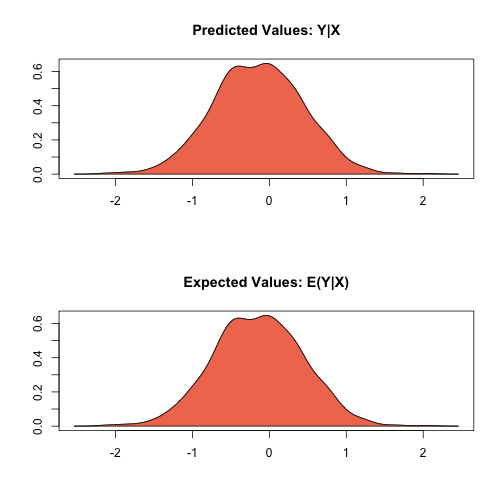
\includegraphics{unnamed-chunk-18.png}
\end{figure}

The cost of giving a range of values for \(\tau\) is that point
estimates are not available for quantities of interest. Instead,
quantities are presented as confidence intervals with significance less
than or equal to a specified level (e.g., at least 95\% of the
simulations are contained in the nominal 95\% confidence interval).


\subsection{Model}
\label{vignette:id53}\begin{itemize}
\item {} 
Like the standard logistic regression, the \emph{stochastic component} for
the rare events logistic regression is:
\begin{gather}
\begin{split}Y_i \; \sim \; \textrm{Bernoulli}(\pi_i),\end{split}\notag
\end{gather}
where \(Y_i\) is the binary dependent variable, and takes a value
of either 0 or 1.

\item {} 
The \emph{systematic component} is:
\begin{gather}
\begin{split}\pi_i \; = \; \frac{1}{1 + \exp(-x_i \beta)}.\end{split}\notag
\end{gather}
\item {} 
If the sample is generated via a case-control (or choice-based)
design, such as when drawing all events (or “cases”) and a sample
from the non-events (or “controls”) and going backwards to collect
the explanatory variables, you must correct for selecting on the
dependent variable. While the slope coefficients are approximately
unbiased, the constant term may be significantly biased. Zelig has
two methods for case control correction:
\begin{enumerate}
\item {} 
The “prior correction” method adjusts the intercept term. Let
\(\tau\) be the true population fraction of events,
\(\bar{y}\) the fraction of events in the sample, and
\(\hat{\beta_0}\) the uncorrected intercept term. The
corrected intercept \(\beta_0\) is:
\begin{gather}
\begin{split}\beta =  \hat{\beta_0} - \ln \left[ \bigg( \frac{1 - \tau}{\tau}
  \bigg) \bigg( \frac{\bar{y}}{1 - \bar{y}} \bigg) \right].\end{split}\notag
\end{gather}
\item {} 
The “weighting” method performs a weighted logistic regression to
correct for a case-control sampling design. Let the 1 subscript
denote observations for which the dependent variable is observed
as a 1, and the 0 subscript denote observations for which the
dependent variable is observed as a 0. Then the vector of weights
\(w_i\)
\begin{gather}
\begin{split}\begin{aligned}
w_1 &=& \frac{\tau}{\bar{y}} \\
w_0 &=& \frac{(1 - \tau)}{(1 - \bar{y})} \\
w_i &=& w_1 Y_i + w_0 (1 - Y_i)\end{aligned}\end{split}\notag
\end{gather}
\end{enumerate}

If \(\tau\) is unknown, you may alternatively specify an upper
and lower bound for the possible range of \(\tau\). In this case,
the relogit procedure uses “robust Bayesian” methods to generate a
confidence interval (rather than a point estimate) for each quantity
of interest. The nominal coverage of the confidence interval is at
least as great as the actual coverage.

\item {} 
By default, estimates of the the coefficients \(\beta\) are
bias-corrected to account for finite sample or rare events bias. In
addition, quantities of interest, such as predicted probabilities,
are also corrected of rare-events bias. If \(\widehat{\beta}\)
are the uncorrected logit coefficients and
bias(\(\widehat{\beta}\)) is the bias term, the corrected
coefficients \(\tilde{\beta}\) are
\begin{gather}
\begin{split}\widehat{\beta} - \textrm{bias}(\widehat{\beta}) = \tilde{\beta}\end{split}\notag
\end{gather}
The bias term is
\begin{gather}
\begin{split}\textrm{bias}(\widehat{\beta}) = (X'WX)^{-1} X'W \xi\end{split}\notag
\end{gather}
where
\begin{gather}
\begin{split}\begin{aligned}
\xi_i &=& 0.5 Q_{ii} \Big( (1 + w-1)\widehat{\pi}_i - w_1 \Big) \\
Q &=& X(X'WX)^{-1} X' \\
W = \textrm{diag}\{\widehat{\pi}_i (1 - \widehat{\pi}_i) w_i\}\end{aligned}\end{split}\notag
\end{gather}
where \(w_i\) and \(w_1\) are given in the “weighting”
section above.

\end{itemize}


\subsection{Quantities of Interest}
\label{vignette:id54}\begin{itemize}
\item {} 
For either one or no \(\tau\):
\begin{itemize}
\item {} 
The expected values (qi\$ev) for the rare events logit are
simulations of the predicted probability
\begin{gather}
\begin{split}E(Y) = \pi_i =
    \frac{1}{1 + \exp(-x_i \beta)},\end{split}\notag
\end{gather}
given draws of \(\beta\) from its posterior.

\item {} 
The predicted value (qi\$pr) is a draw from a binomial distribution
with mean equal to the simulated \(\pi_i\).

\item {} 
The first difference (qi\$fd) is defined as
\begin{gather}
\begin{split}\textrm{FD} = \Pr(Y = 1 \mid x_1, \tau) - \Pr(Y = 1 \mid x, \tau).\end{split}\notag
\end{gather}
\item {} 
The risk ratio (qi\$rr) is defined as
\begin{gather}
\begin{split}\textrm{RR} = \Pr(Y = 1 \mid x_1, \tau) \ / \ \Pr(Y = 1 \mid x, \tau).\end{split}\notag
\end{gather}
\end{itemize}

\item {} 
For a range of \(\tau\) defined by \([\tau_1, \tau_2]\), each
of the quantities of interest are \(n \times 2\) matrices, which
report the lower and upper bounds, respectively, for a confidence
interval with nominal coverage at least as great as the actual
coverage. At worst, these bounds are conservative estimates for the
likely range for each quantity of interest. Please refer to for the
specific method of calculating bounded quantities of interest.

\item {} 
In conditional prediction models, the average expected treatment
effect (att.ev) for the treatment group is
\begin{gather}
\begin{split}\frac{1}{\sum_{i=1}^n t_i}\sum_{i:t_i=1}^n \left\{ Y_i(t_i=1) -
      E[Y_i(t_i=0)] \right\},\end{split}\notag
\end{gather}
where \(t_i\) is a binary explanatory variable defining the
treatment (\(t_i=1\)) and control (\(t_i=0\)) groups.
Variation in the simulations are due to uncertainty in simulating
\(E[Y_i(t_i=0)]\), the counterfactual expected value of
\(Y_i\) for observations in the treatment group, under the
assumption that everything stays the same except that the treatment
indicator is switched to \(t_i=0\).

\item {} 
In conditional prediction models, the average predicted treatment
effect (att.pr) for the treatment group is
\begin{gather}
\begin{split}\frac{1}{\sum_{i=1}^n t_i}\sum_{i:t_i=1}^n \left\{ Y_i(t_i=1) -
      \widehat{Y_i(t_i=0)} \right\},\end{split}\notag
\end{gather}
where \(t_i\) is a binary explanatory variable defining the
treatment (\(t_i=1\)) and control (\(t_i=0\)) groups.
Variation in the simulations are due to uncertainty in simulating
\(\widehat{Y_i(t_i=0)}\), the counterfactual predicted value of
\(Y_i\) for observations in the treatment group, under the
assumption that everything stays the same except that the treatment
indicator is switched to \(t_i=0\).

\end{itemize}


\subsection{Output Values}
\label{vignette:id55}
The output of each Zelig command contains useful information which you
may view. For example, if you run
\code{z.out \textless{}- zelig(y \textasciitilde{} x, model = relogit, data)}, then you may examine
the available information in \code{z.out} by using \code{names(z.out)}, see
the coefficients by using z.out\$coefficients, and a default summary of
information through \code{summary(z.out)}.


\subsection{Differences with Stata Version}
\label{vignette:differences-with-stata-version}
The Stata version of ReLogit and the R implementation differ slightly in
their coefficient estimates due to differences in the matrix inversion
routines implemented in R and Stata. Zelig uses orthogonal-triangular
decomposition (through lm.influence()) to compute the bias term, which
is more numerically stable than standard matrix calculations.


\subsection{See also}
\label{vignette:id56}

\bigskip\hrule{}\bigskip



\section{zelig-tobit}
\label{vignette:zelig-tobit}
Linear Regression for a Left-Censored Dependent Variable

Tobit regression estimates a linear regression model for a left-censored
dependent variable, where the dependent variable is censored from below.
While the classical tobit model has values censored at 0, you may select
another censoring point. For other linear regression models with fully
observed dependent variables, see Bayesian regression (), maximum
likelihood normal regression (), or least squares ().


\subsection{Syntax}
\label{vignette:id57}
\begin{Verbatim}[commandchars=\\\{\}]
z5 \PYG{o}{\PYGZlt{}\PYGZhy{}} ztobit\PYG{o}{\PYGZdl{}}new\PYG{p}{(}\PYG{p}{)}
z5\PYG{o}{\PYGZdl{}}zelig\PYG{p}{(}Y \PYG{o}{\PYGZti{}} X1 \PYG{o}{+} X2\PYG{p}{,} below \PYG{o}{=} \PYG{l+m}{0}\PYG{p}{,} above \PYG{o}{=} \PYG{k+kc}{Inf}\PYG{p}{,} data \PYG{o}{=} mydata\PYG{p}{)}
z5\PYG{o}{\PYGZdl{}}setx\PYG{p}{(}\PYG{p}{)}
z5\PYG{o}{\PYGZdl{}}sim\PYG{p}{(}\PYG{p}{)}
\end{Verbatim}

With the Zelig 4 compatibility wrappers:

\begin{Verbatim}[commandchars=\\\{\}]
z.out \PYG{o}{\PYGZlt{}\PYGZhy{}} zelig\PYG{p}{(}Y \PYG{o}{\PYGZti{}} X1 \PYG{o}{+} X2\PYG{p}{,} below \PYG{o}{=} \PYG{l+m}{0}\PYG{p}{,} above \PYG{o}{=} \PYG{k+kc}{Inf}\PYG{p}{,} model \PYG{o}{=} \PYG{l+s}{\PYGZdq{}}\PYG{l+s}{tobit\PYGZdq{}}\PYG{p}{,} data \PYG{o}{=} mydata\PYG{p}{)}
x.out \PYG{o}{\PYGZlt{}\PYGZhy{}} setx\PYG{p}{(}z.out\PYG{p}{)}
s.out \PYG{o}{\PYGZlt{}\PYGZhy{}} sim\PYG{p}{(}z.out\PYG{p}{,} x \PYG{o}{=} x.out\PYG{p}{)}
\end{Verbatim}


\subsection{Inputs}
\label{vignette:inputs}
zelig() accepts the following arguments to specify how the dependent
variable is censored.
\begin{itemize}
\item {} 
\code{below}: (defaults to 0) The point at which the dependent variable
is censored from below. If any values in the dependent variable are
observed to be less than the censoring point, it is assumed that that
particular observation is censored from below at the observed value.
(See for a Bayesian implementation that supports both left and right
censoring.)

\item {} 
robust: defaults to FALSE. If TRUE, zelig() computes robust standard
errors based on sandwich estimators (see and ) and the options
selected in cluster.

\item {} 
cluster: if robust = TRUE, you may select a variable to define groups
of correlated observations. Let x3 be a variable that consists of
either discrete numeric values, character strings, or factors that
define strata. Then

\begin{Verbatim}[commandchars=\\\{\}]
\PYGZgt{} z.out \PYGZlt{}\PYGZhy{} zelig(y \PYGZti{} x1 + x2, robust = TRUE, cluster = \PYGZdq{}x3\PYGZdq{},
                 model = \PYGZdq{}tobit\PYGZdq{}, data = mydata)
\end{Verbatim}

means that the observations can be correlated within the strata
defined by the variable x3, and that robust standard errors should be
calculated according to those clusters. If robust = TRUE but cluster
is not specified, zelig() assumes that each observation falls into
its own cluster.

\end{itemize}

Zelig users may wish to refer to \code{help(survreg)} for more information.


\subsection{Examples}
\label{vignette:id58}

\subsubsection{Basic Example}
\label{vignette:id59}
Attaching the sample dataset:

\begin{Verbatim}[commandchars=\\\{\}]
data\PYG{p}{(}tobin\PYG{p}{)}
\end{Verbatim}

Estimating linear regression using \code{tobit}:

\begin{Verbatim}[commandchars=\\\{\}]
z.out \PYG{o}{\PYGZlt{}\PYGZhy{}} zelig\PYG{p}{(}durable \PYG{o}{\PYGZti{}} age \PYG{o}{+} quant\PYG{p}{,} model \PYG{o}{=} \PYG{l+s}{\PYGZdq{}}\PYG{l+s}{tobit\PYGZdq{}}\PYG{p}{,} data \PYG{o}{=} tobin\PYG{p}{)}
\end{Verbatim}

\begin{Verbatim}[commandchars=\\\{\}]
\PYG{c}{\PYGZsh{}\PYGZsh{} How to cite this model in Zelig:}
\PYG{c}{\PYGZsh{}\PYGZsh{}   Kosuke Imai, Gary King, Olivia Lau. 2011.}
\PYG{c}{\PYGZsh{}\PYGZsh{}   tobit: Linear regression for Left\PYGZhy{}Censored Dependent Variable}
\PYG{c}{\PYGZsh{}\PYGZsh{}   in Kosuke Imai, Gary King, and Olivia Lau, \PYGZdq{}Zelig: Everyone\PYGZsq{}s Statistical Software,\PYGZdq{}}
\PYG{c}{\PYGZsh{}\PYGZsh{}   http://datascience.iq.harvard.edu/zelig}
\end{Verbatim}

Setting values for the explanatory variables to their sample averages:

\begin{Verbatim}[commandchars=\\\{\}]
x.out \PYG{o}{\PYGZlt{}\PYGZhy{}} setx\PYG{p}{(}z.out\PYG{p}{)}
\end{Verbatim}

Simulating quantities of interest from the posterior distribution given \code{x.out}.

\begin{Verbatim}[commandchars=\\\{\}]
s.out1 \PYG{o}{\PYGZlt{}\PYGZhy{}} sim\PYG{p}{(}z.out\PYG{p}{,} x \PYG{o}{=} x.out\PYG{p}{)}
\end{Verbatim}

\begin{Verbatim}[commandchars=\\\{\}]
summary\PYG{p}{(}s.out1\PYG{p}{)}
\end{Verbatim}

\begin{Verbatim}[commandchars=\\\{\}]
\PYG{c}{\PYGZsh{}\PYGZsh{}}
\PYG{c}{\PYGZsh{}\PYGZsh{}  sim x :}
\PYG{c}{\PYGZsh{}\PYGZsh{}  \PYGZhy{}\PYGZhy{}\PYGZhy{}\PYGZhy{}\PYGZhy{}}
\PYG{c}{\PYGZsh{}\PYGZsh{} ev}
\PYG{c}{\PYGZsh{}\PYGZsh{}   mean     sd   50\PYGZpc{}   2.5\PYGZpc{} 97.5\PYGZpc{}}
\PYG{c}{\PYGZsh{}\PYGZsh{} 1 1.56 0.6528 1.482 0.5335 2.922}
\PYG{c}{\PYGZsh{}\PYGZsh{} pv}
\PYG{c}{\PYGZsh{}\PYGZsh{}       mean    sd   50\PYGZpc{} 2.5\PYGZpc{} 97.5\PYGZpc{}}
\PYG{c}{\PYGZsh{}\PYGZsh{} [1,] 3.082 4.057 1.141    0 13.35}
\end{Verbatim}


\subsubsection{Simulating First Differences}
\label{vignette:id60}
Set explanatory variables to their default(mean/mode) values, with
high (80th percentile) and low (20th percentile) liquidity ratio
(\code{quant}):

\begin{Verbatim}[commandchars=\\\{\}]
x.high \PYG{o}{\PYGZlt{}\PYGZhy{}} setx\PYG{p}{(}z.out\PYG{p}{,} quant \PYG{o}{=} quantile\PYG{p}{(}tobin\PYG{o}{\PYGZdl{}}quant\PYG{p}{,} prob \PYG{o}{=} \PYG{l+m}{0.8}\PYG{p}{)}\PYG{p}{)}
x.low \PYG{o}{\PYGZlt{}\PYGZhy{}} setx\PYG{p}{(}z.out\PYG{p}{,} quant \PYG{o}{=} quantile\PYG{p}{(}tobin\PYG{o}{\PYGZdl{}}quant\PYG{p}{,} prob \PYG{o}{=} \PYG{l+m}{0.2}\PYG{p}{)}\PYG{p}{)}
\end{Verbatim}

Estimating the first difference for the effect of high versus low
liquidity ratio on duration(\code{durable}):

\begin{Verbatim}[commandchars=\\\{\}]
s.out2 \PYG{o}{\PYGZlt{}\PYGZhy{}} sim\PYG{p}{(}z.out\PYG{p}{,} x \PYG{o}{=} x.high\PYG{p}{,} x1 \PYG{o}{=} x.low\PYG{p}{)}
\end{Verbatim}

\begin{Verbatim}[commandchars=\\\{\}]
summary\PYG{p}{(}s.out2\PYG{p}{)}
\end{Verbatim}

\begin{Verbatim}[commandchars=\\\{\}]
\PYG{c}{\PYGZsh{}\PYGZsh{}}
\PYG{c}{\PYGZsh{}\PYGZsh{}  sim x :}
\PYG{c}{\PYGZsh{}\PYGZsh{}  \PYGZhy{}\PYGZhy{}\PYGZhy{}\PYGZhy{}\PYGZhy{}}
\PYG{c}{\PYGZsh{}\PYGZsh{} ev}
\PYG{c}{\PYGZsh{}\PYGZsh{}    mean     sd   50\PYGZpc{}   2.5\PYGZpc{} 97.5\PYGZpc{}}
\PYG{c}{\PYGZsh{}\PYGZsh{} 1 1.176 0.7449 1.047 0.1403 2.873}
\PYG{c}{\PYGZsh{}\PYGZsh{} pv}
\PYG{c}{\PYGZsh{}\PYGZsh{}       mean    sd   50\PYGZpc{} 2.5\PYGZpc{} 97.5\PYGZpc{}}
\PYG{c}{\PYGZsh{}\PYGZsh{} [1,] 2.833 3.798 1.238    0 13.31}
\PYG{c}{\PYGZsh{}\PYGZsh{}}
\PYG{c}{\PYGZsh{}\PYGZsh{}  sim x1 :}
\PYG{c}{\PYGZsh{}\PYGZsh{}  \PYGZhy{}\PYGZhy{}\PYGZhy{}\PYGZhy{}\PYGZhy{}}
\PYG{c}{\PYGZsh{}\PYGZsh{} ev}
\PYG{c}{\PYGZsh{}\PYGZsh{}    mean     sd  50\PYGZpc{}   2.5\PYGZpc{} 97.5\PYGZpc{}}
\PYG{c}{\PYGZsh{}\PYGZsh{} 1 2.092 0.9679 2.01 0.5675 4.187}
\PYG{c}{\PYGZsh{}\PYGZsh{} pv}
\PYG{c}{\PYGZsh{}\PYGZsh{}       mean    sd   50\PYGZpc{} 2.5\PYGZpc{} 97.5\PYGZpc{}}
\PYG{c}{\PYGZsh{}\PYGZsh{} [1,] 3.736 4.464 2.224    0 14.94}
\PYG{c}{\PYGZsh{}\PYGZsh{} fd}
\PYG{c}{\PYGZsh{}\PYGZsh{}    mean    sd    50\PYGZpc{}   2.5\PYGZpc{} 97.5\PYGZpc{}}
\PYG{c}{\PYGZsh{}\PYGZsh{} 1 0.916 1.143 0.8715 \PYGZhy{}1.321 3.252}
\end{Verbatim}

\begin{Verbatim}[commandchars=\\\{\}]
plot\PYG{p}{(}s.out1\PYG{p}{)}
\end{Verbatim}
\begin{figure}[htbp]
\centering
\capstart

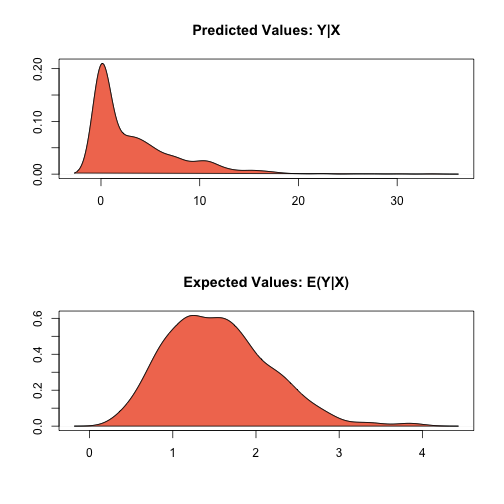
\includegraphics{Zelig-tobit.png}
\caption{Zelig-tobit}\end{figure}


\subsection{Model}
\label{vignette:id61}\begin{itemize}
\item {} 
Let \(Y_i^*\) be a latent dependent variable which is distributed
with \emph{stochastic} component
\begin{gather}
\begin{split}\begin{aligned}
Y_i^* & \sim & \textrm{Normal}(\mu_i, \sigma^2) \\\end{aligned}\end{split}\notag
\end{gather}
where \(\mu_i\) is a vector means and \(\sigma^2\) is a
scalar variance parameter. \(Y_i^*\) is not directly observed,
however. Rather we observed \(Y_i\) which is defined as:
\begin{gather}
\begin{split}Y_i = \left\{
\begin{array}{lcl}
Y_i^*  &\textrm{if} & c <Y_i^* \\
c    &\textrm{if} & c \ge Y_i^*
\end{array}\right.\end{split}\notag
\end{gather}
where \(c\) is the lower bound below which \(Y_i^*\) is
censored.

\item {} 
The \emph{systematic component} is given by
\begin{gather}
\begin{split}\begin{aligned}
\mu_{i} &=& x_{i} \beta,\end{aligned}\end{split}\notag
\end{gather}
where \(x_{i}\) is the vector of \(k\) explanatory variables
for observation \(i\) and \(\beta\) is the vector of
coefficients.

\end{itemize}


\subsection{Quantities of Interest}
\label{vignette:id62}\begin{itemize}
\item {} 
The expected values (\code{qi\$ev}) for the tobit regression model are
the same as the expected value of \(Y*\):
\begin{gather}
\begin{split}E(Y^* | X) = \mu_{i} = x_{i} \beta\end{split}\notag
\end{gather}
\item {} 
The first difference (\code{qi\$fd}) for the tobit regression model is
defined as
\begin{gather}
\begin{split}\begin{aligned}
\text{FD}=E(Y^* \mid x_{1}) - E(Y^* \mid x).\end{aligned}\end{split}\notag
\end{gather}
\item {} 
In conditional prediction models, the average expected treatment
effect (\code{qi\$att.ev}) for the treatment group is
\begin{gather}
\begin{split}\begin{aligned}
\frac{1}{\sum t_{i}}\sum_{i:t_{i}=1}[E[Y^*_{i}(t_{i}=1)]-E[Y^*_{i}(t_{i}=0)]],\end{aligned}\end{split}\notag
\end{gather}
where \(t_{i}\) is a binary explanatory variable defining the
treatment (\(t_{i}=1\)) and control (\(t_{i}=0\)) groups.

\end{itemize}


\subsection{Output Values}
\label{vignette:id63}
The output of each Zelig command contains useful information which you
may view. For example, if you run:

\begin{Verbatim}[commandchars=\\\{\}]
z.out \PYG{o}{\PYGZlt{}\PYGZhy{}} zelig\PYG{p}{(}y \PYG{o}{\PYGZti{}} x\PYG{p}{,} model \PYG{o}{=} \PYG{l+s}{\PYGZdq{}}\PYG{l+s}{tobit\PYGZdq{}}\PYG{p}{,} data\PYG{p}{)}
\end{Verbatim}

then you may examine the available information in {\color{red}\bfseries{}{}`{}`}z.out{}`.


\subsection{See also}
\label{vignette:id66}
The tobit function is part of the survival library by Terry Therneau,
ported to R by Thomas Lumley. Advanced users may wish to refer to
\code{help(survfit)} in the survival library.


\chapter{Frequently Asked Questions}
\label{faq:faq}\label{faq::doc}\label{faq:frequently-asked-questions}
If you find a bug, or cannot figure something out after reading through the FAQs below, please send your question to the Zelig listserv at: \href{https://groups.google.com/forum/\#!forum/zelig-statistical-software}{https://groups.google.com/forum/\#!forum/zelig-statistical-software}. Please explain exactly what you did and include the full error message, including the traceback(). You should get an answer from the developers or another user in short order.


\bigskip\hrule{}\bigskip



\section{Why can’t I install Zelig?}
\label{faq:why-cant-i-install-zelig}
We recommend that you first check your internet connection, as you must be connected to install packages. In addition, there are a few platform-specific reasons why you may be having installation problems:
\begin{itemize}
\item {} 
\textbf{On Windows}: If you are using the very latest version of R, you may not be able to install Zelig until we update Zelig to work with this latest release. Currently Zelig 5.0.1 is compatible with R(\textgreater{}= 3.0.2). If you wish to install Zelig in the interim, install the appropriate version of R and try to reinstall Zelig.

\item {} 
\textbf{On Mac or Linux systems}: If you get the following warning message at the end of your installation:

\begin{Verbatim}[commandchars=\\\{\}]
\PYG{o}{\PYGZgt{}} Installation of package VGAM had non\PYG{o}{\PYGZhy{}}zero exit status \PYG{k+kr}{in} \PYG{k+kc}{...}
\end{Verbatim}

this means that you were not able to install VGAM properly. Make sure that you have the g77 Fortran compiler. For Intel Macs, download the Apple developer tools. After installation, try to install Zelig again.

\end{itemize}

If neither solution works, feel free email the Zelig mailing list directly at: \href{https://groups.google.com/forum/\#!forum/zelig-statistical-software}{https://groups.google.com/forum/\#!forum/zelig-statistical-software}.


\bigskip\hrule{}\bigskip



\section{Why can’t I install R?}
\label{faq:why-cant-i-install-r}
If you have problems installing R, you should search the internet for the R help mailing list, check out technical Q \& A forums (e.g., StackOverflow), or email the Zelig mailing list directly at: \href{https://groups.google.com/forum/\#!forum/zelig-statistical-software}{https://groups.google.com/forum/\#!forum/zelig-statistical-software}.


\bigskip\hrule{}\bigskip



\section{Why can’t I load data?}
\label{faq:why-cant-i-load-data}
It is likely that the reason you are unable to load data because you have not specified the correct working directory (e.g., the location of the data you are trying to load). You should specify you working directory use the \code{setwd()} function in which you will include the the file path to your working director. For example, if I wanted to load a file that is my \emph{Documents} folder, I must first:

\begin{Verbatim}[commandchars=\\\{\}]
\PYG{o}{\PYGZgt{}} setwd\PYG{p}{(}\PYG{l+s}{\PYGZdq{}}\PYG{l+s}{path/to/Documents\PYGZdq{}}\PYG{p}{)}
\end{Verbatim}

File paths can be found by right clicking the working directory folder in any file browser and clicking ``Get Info'' (on Mac) or ``Properties'' (on Windows). Black-slashes (\textbackslash{}) in file paths copied from the ``Properties'' link on Windows machines must be replace with forward-slashes (/). For example, the Windows path: \code{C:\textbackslash{}Program Files\textbackslash{}R}, would be typed as \code{C:/Program Files/R}.


\bigskip\hrule{}\bigskip



\section{R is neat. How can I find out more?}
\label{faq:r-is-neat-how-can-i-find-out-more}
R is a collective project with contributors from all over the world. Their website (\href{http://www.r-project.org}{http://www.r-project.org}) has more information on the R project, R packages, conferences, and other learning material.


\chapter{About Zelig}
\label{about:about}\label{about::doc}\label{about:about-zelig}
Zelig is an open source project development and maintained by the Data Science group at the \href{http://datascience.iq.harvard.edu/}{Data Science group} at Harvard's Institute for Quantitative Social Science (IQSS). It was originally conceived and created by Kosuke Imai, Gary King, and Olivia Lau in 2007. The name is borrowed from Woody Allen's movie with the same name, Zelig. Leonard Zelig is a fictional character who takes on the characteristics of any strong personality around. Likewise, the Zelig statistical software easily adapts to any statistical model written in R, and in essence, takes the characteristics of any model.

It leverages (R) code from many researchers and is designed to allow anyone to contribute their methods to it. Hence, we often refer to Zelig as ``everyone's statistical software'' and our aim is to make it, as well as the models it wraps, as accessible as possible. As such, Zelig comes with self-contained documentation that minimizes startup costs, automates model summaries and graphics, and bridges existing R implementations through an intelligible call structure.

\textbf{License:} GPL-2 \textbar{} GPL-3 {[}expanded from: GPL (\textgreater{}= 2){]}

\textbf{Contact:} For questions, please join the Zelig mailing list:
\href{https://groups.google.com/forum/\#!forum/zelig-statistical-software}{https://groups.google.com/forum/\#!forum/zelig-statistical-software}

\href{http://datascience.iq.harvard.edu/team}{The Zelig Team}:
\begin{itemize}
\item {} 
Christine Choirat \emph{(Lead Author)}

\item {} 
James Honaker \emph{(Project Lead)}

\item {} 
Muhammed Y. Idris

\end{itemize}

\emph{Original Authors:}
\begin{itemize}
\item {} 
\href{http://gking.harvard.edu/}{Gary King} \emph{(Principle Investigator)}

\item {} 
Kosuke Imai

\item {} 
Olivia Lau

\end{itemize}


\bigskip\hrule{}\bigskip



\section{Technical Vision}
\label{about:technical-vision}
Zelig is a framework for interfacing a wide range of statistical models and analytic methods in a common and simple way. Above and beyond estimation, Zelig adds considerable infrastructure to existing heterogeneous R implementations by translating hard-to-interpret coefficients into quantities of interest (e.g., expected and predicted values) through a simple call structure. This includes many specific methods, based on likelihood, frequentist, Bayesian, robust Bayesian and nonparametric theories of inference. Developers are encouraged to add their R packages to the Zelig toolkit by writing a few simple bridge functions.

Additional features include:
\begin{itemize}
\item {} 
Dealing with missing data by combining multiply imputed datasets

\item {} 
Automating statistical bootstrapping

\item {} 
Improving parametric procedures by leveraging nonparametric matching methods

\item {} 
Evaluating counterfactuals

\item {} 
Allowing conditional population and super population inferences

\item {} 
Automating the creation of replication data files

\end{itemize}


\section{Release Notes}
\label{about:release-notes}
\textbf{v 5.0.1}

This release expands the set of models available, while simplifying the model wrapping process, and solving architectural problems by completely rewriting into R’s Reference Classes for a fully object-oriented architecture.

\emph{Inheritance Tree}



\renewcommand{\indexname}{Index}
\printindex
\end{document}
